\documentclass[a4paper,oneside,12pt]{report}
\usepackage[utf8x]{inputenc} % To use Unicode (e.g. Turkish) characters
\usepackage{amsmath, amsthm} % Some extra symbols
%\usepackage{subcaption}
\usepackage{styles/fbe_tez}
\usepackage[bottom]{footmisc}
\usepackage{cite}
\usepackage{graphicx}
\usepackage{longtable}
\usepackage{float}
\usepackage{multirow}
\usepackage{algorithm}
\usepackage{algorithmic}
\usepackage{array}
\usepackage{amssymb,bm,cite,graphicx, fixmath, texdraw}
\usepackage{epsfig}
\usepackage{epstopdf}
\usepackage{amsmath}
\usepackage{notoccite}
\usepackage{subcaption}
\usepackage{tabu}
\usepackage{minted}
\usepackage{xcolor}

\usemintedstyle{xcode}
\definecolor{bg}{rgb}{0.95,0.95,0.95}


\interdisplaylinepenalty=2500
\hyphenation{lists} \makeatletter

\newcommand{\field}[1]{\mathbb{#1} }
\newcommand{\beq}{\begin{equation} \setlength\abovedisplayskip{5pt} 
\setlength\belowdisplayskip{5pt}}
\newcommand{\eeq}{\end{equation}}
\newcommand{\bea}{\begin{eqnarray}}
\newcommand{\eea}{\end{eqnarray}}
\newcommand{\defn}{\stackrel{\triangle}{=}}
\newcommand{\nn}{\nonumber}
\newcommand{\nnl}{\nonumber \\}
\renewcommand{\theequation}{\arabic{equation}}
\renewcommand{\labelenumi}{(\roman{enumi})}

\DeclareMathOperator*{\argmin}{arg\,min}
\DeclareMathOperator*{\argmax}{arg\,max}

\def\ifundefined{\@ifundefined}
\def\bfat{\left[ \begin{array}}
\def\emat{\end{array} \right]}
\def\bfatt{\left\{ \begin{array}}
\def\ematt{\end{array} \right.}
\def\bset{\left\{ \begin{array}}
\def\eset{\end{array} \right\}}
\def\bpar{\left( \begin{array}}
\def\epar{\end{array} \right)}

\graphicspath{{figures/}} % Graphics will be here

\newtheorem{thm}{Theorem}[chapter]
\newtheorem{prop}[thm]{Proposition}
\newtheorem{lem}[thm]{Lemma}
\newtheorem{cor}[thm]{Corollary}

\numberwithin{equation}{chapter}


% COVER PAGE
\title{DESING AND SIMULATION SOFTWARE FOR RHODOTRON TYPE ELECTRON ACCELERATORS}
\turkcebaslik{RHODOTRON TİPİ ELEKTRON HIZLANDIRICILARI İÇİN TASARIM VE SİMÜLASYON YAZILIMI}
\degree{B.S., Physics, Boğaziçi University, 2020}
\author{Muhammet Furkan Er}
\program{M.S. Physics}
\subyear{2023}

% APPROVED BY PAGE
\supervisor{Prof. Veysi Erkcan Özcan}
\cosuperi{Assoc. Prof. Gökhan Ünel}
%\cosuperii{Title and Name of Cosupervisor II}
\examineri{Asst. Prof. Bora Akgün}
\examinerii{Assoc. Prof. Bora Işıldak}
%\examineriv{}
%\examinerv{}
\dateofapproval{DD.MM.YYYY}

% BEGIN OF DOCS
\begin{document}
\pagenumbering{roman}
\makemstitle % M.S. thesis
\makeapprovalpage

% ACK PAGE
\begin{acknowledgements}
Acknowledgements come here...
\end{acknowledgements}

% ABS PAGE
\begin{abstract}
    The focus of this study is to design and optimize rose-pattle-type electron accelerators; a new simulation tool called \textit{Rhodotron Simulation} has been developed for this purpose.
    A coaxial cavity with an operating frequency of $107.5$ MHz is currently being manufactured in the Kandilli Detector Accelerator and Instrumentation Laboratory (KAHVELab).
    This new tool's capabilities will be tested with the cavity and will be used to design complementary bending magnets for reaching $1-5$ MeV beam energy.
\end{abstract}

% OZET PAGE 
\begin{ozet}
Bu çalışma, gül yaprağı tipi elektron hızlandırıcıları tasarlamak ve optimize etmek üzerine odaklanmaktadır. 
Bu amaçla \textit{Rhodotron Simulation} adında yeni bir benzetim uygulaması geliştirilmiş, $107.5$ MHz hedef frekansında çalışmak üzere tasarlanmış bir koaksiyal kavitesinin üretimi, Kandilli Algıç Hızlandırıcı ve Enstrümentasyon Laboratuvarı'nda devam etmektedir.
Yeni benzetim uygulaması, kabiliyetleri üretilen kavite ile test edildikten sonra bükme mıknatısları tasarım ve optimizasyonunda $1-5$ MeV demet enerjisine ulaşmak için kullanılacaktır.
\end{ozet}

% CONTENTS AND LIST OF FIG AND TABLE PAGES
\tableofcontents
\listoffigures 
\listoftables

% LIST OF SYMBOLS PAGE
\begin{symbols}
    % The title will be typeset as "LIST OF SYMBOLS".
    % Use a separate \sym command for each symbols definition.
    % First, Latin symbols in alphabetical order
    \sym{$\vec{a}$}{Acceleration}
    \sym{\textbf{$\vec{B}$}}{Magnetic field}
    \sym{c}{Speed of light in vacuum}
    \sym{E}{Energy}
    \sym{W}{Energy}
    \sym{\textbf{$\vec{E}$}}{Electric field}
    \sym{f}{Frequency}
    \sym{$\vec{F}$}{Force}
    \sym{$\vec{p}$}{Momentum}
    \sym{$\vec{r}$}{Position}
    \sym{t}{Time}
    \sym{T}{Period}
    \sym{$\vec{v}$}{Velocity}
    \sym{Z}{Shunt Impedance}
    % 1 EMPTY LINE BETWEEN LATIN AND GREEK SYMBOLS GROUP!!!
    \sym{}{}
    % Then Greek symbols in alphabetical order
    \sym{$\gamma$}{Lorentz Factor}
    \sym{$\beta$}{Beta Factor}
    \sym{$\phi_{lag}$}{Phase Lag}

    \sym{$\mu X$}{Mean Value of X}
    \sym{$\sigma X$}{Standard Deviation of X}
    \sym{}{}
\end{symbols}

% LIST OF ABBREV PAGE
\begin{abbreviations}
    % Abbreviations in alphabetical order
   \sym{2D}{One Dimensional}
   \sym{2D}{Two Dimensional}
   \sym{3D}{Three Dimensional}
   \sym{eV}{Electron Volt}
   \sym{Hz}{Hertz}
   \sym{KAHVELab}{Kandilli Detector Accelerator and \\Instrumentation Laboratory}
   \sym{Linac}{Linear Particle Accelerator}
   \sym{ODE}{Ordinary Differential Equation}
   \sym{RF}{Radio Frequency}
   \sym{POC}{Proof of Concept}
   \sym{CPU}{Central Processing Unit}
   \sym{s}{Second}
   \sym{T}{Tesla}
   \sym{V}{Volt}
   \sym{W}{Watt}

\end{abbreviations}


\pagenumbering{arabic}



\newcommand{\vecthreeBF}[1]{\vec{\textbf{#1}}}
\newcommand{\vecthree}[1]{\vec{#1}}
\newcommand{\vecNum}[3]{(#1, #2, #3)}

\newcommand{\parDeriv}[2]{\frac{\partial #1}{\partial #2}}
\newcommand{\parDerivS}[2]{\frac{\partial^2 #1}{\partial #2^2}}
\newcommand{\derivS}[2]{\frac{d^2 #1}{d#2^2}}

\newcommand{\dotProdBF}[2]{\vecthreeBF{#1} \cdot \vecthreeBF{#2}}
\newcommand{\dotProd}[2]{\vecthree{#1} \cdot \vecthree{#2}}

\newcommand{\crossProdBF}[2]{\vecthreeBF{#1} \times \vecthreeBF{#2}}
\newcommand{\crossProd}[2]{\vecthree{#1} \times \vecthree{#2}}

\newcommand{\e}{$\textbf{e}^-$ }
\newcommand{\egun}{$\textbf{e}^-$-gun }
\newcommand{\eB}{$\textbf{e}^-$ - $\vecthreeBF{B}$ }
\newcommand{\eE}{$\textbf{e}^-$ - $\vecthreeBF{E}$ }
\newcommand{\eEM}{$\textbf{e}^-$ - \textbf{EM} }
\newcommand{\ee}{$\textbf{e}^-$ - $\textbf{e}^-$ }


\newcommand{\fromeq}[1]{\textit{equation \ref{eq:#1}}}
\newcommand{\fromeqs}[2]{\textit{equations \ref{eq:#1} and \ref{eq:#2}}}
\newcommand{\fromeqsth}[3]{\textit{equations \ref{eq:#1}, \ref{eq:#2} and \ref{eq:#3}}}
\newcommand{\fromeqsf}[4]{\textit{equations \ref{eq:#1}, \ref{eq:#2}, \ref{eq:#3} and \ref{eq:#4}}}

\newcommand{\fromfig}[1]{\textit{figure \ref{fig:#1}}}
\newcommand{\fromfigs}[2]{\textit{figures \ref{fig:#1} and \ref{fig:#2}}}
\newcommand{\fromfigf}[4]{\textit{figures \ref{fig:#1}, \ref{fig:#2}, \ref{fig:#3} and \ref{fig:#4}}}
\newcommand{\fromfigsix}[6]{\textit{figures \ref{fig:#1}, \ref{fig:#2}, \ref{fig:#3}, \ref{fig:#4}, \ref{fig:#5} and \ref{fig:#6}}}

\newcommand{\fromch}[1]{\textit{chapter \ref{ch:#1}}}

\newcommand{\fromsec}[1]{\textit{section \ref{sec:#1}}}
\newcommand{\fromsecs}[2]{\textit{sections \ref{sec:#1} and \ref{sec:#2}}}

\newcommand{\fromapp}[1]{\textit{Appendix \ref{appendix:#1}}}

\newcommand{\fromtab}[1]{\textit{Table \ref{tab:#1}}}
\newcommand{\fromtabs}[2]{\textit{Tables \ref{tab:#1} and \ref{tab:#2}}}
\newcommand{\fromtabf}[4]{\textit{Tables \ref{tab:#1}, \ref{tab:#2}, \ref{tab:#3} and \ref{tab:#4}}}


% START OF INTRODUCTION AND THEORY

\chapter{INTRODUCTION AND THEORY}

Particle accelerators are essential tools for scientific research. They enable scientists to probe the fundamental constituents of matter, study particle interactions, and explore the laws of physics. 
Accelerators have been instrumental in discovering and characterizing fundamental particles, such as quarks, leptons, and more recently the Higgs boson. 
They also facilitate the production of high-intensity particle beams for applications in industrial processes. A conservative estimate puts the number of industrial high-current electron
accelerators to be in the thousands, worldwide.

MeV-level electron beams, both as is and as X-Ray sources, are especially useful for industrial and medical applications. 
For instance,  high-energy beams (ranging from 5 to 10 MeV) find application in medical accelerators and in services such as sterilizing medical devices and irradiating food. 
Meanwhile, medium-energy devices (ranging from 400 keV to 5 MeV) contribute to the improvement of wires, cables, and tires, and also play a role in treating factory flue gases and wastewater.
Although most of the industrial electron accelerators operating at MeV-level are linear accelerators at the moment, due to their compact nature, circular accelerators have been gaining prominence. 

Rose-pattle accelerator is a type of circular accelerator suitable for producing electron beams at MeV-level energy. 
It was developed in 1989 and was named \textit{Rhodotron} \cite{rhodo_pottier}. This name was trademarked by \textit{IBA Group} in the following years. 



\section{Accelerating Charged Particles}

\subsection{Relation between momentum and acceleration}
In classical mechanics, Newton's second law defines force, $\vecthreeBF{F}$, and states 
\begin{equation} \label{eq:newton_second_law}
    \vecthreeBF{F} = \frac{\partial \vecthreeBF{p}}{\partial t} = m \frac{\partial \vecthreeBF{v}}{\partial t} = m \vecthreeBF{a}
\end{equation}
where $\vecthreeBF{p}$ is the momentum, $m\vecthreeBF{v}$ of the particle. In special relativity however, relativistic momentum is defined as $\vecthree{p} = \gamma m_0 \vecthree{v} $ where $\gamma$ is the Lorentz Factor:
\begin{equation}
    \gamma = \frac{1}{\sqrt{1-v^2 / c^2}} = = \frac{1}{\sqrt{1-\beta^2}}
            = \frac{1}{\sqrt{1- (\dotProd{v}{v})/ c^2}} =  \frac{1}{\sqrt{1- \dotProd{\beta}{\beta}}}
\end{equation}
Considering these two statements, we can find the relation between momentum and acceleration as follows:
\begin{eqnarray}
    \parDeriv{\vecthree{p}}{t} &=& m_0 \parDeriv{(\gamma \vecthree{v})}{t} = m_0 \{  \parDeriv{\gamma}{t}\vecthree{v} + \gamma \parDeriv{\vecthree{v}}{t}  \} \\
    \parDeriv{\gamma}{t} &=& \gamma^3 \dotProd{\beta}{\parDeriv{\beta}{t}} = \frac{\gamma^3}{c} \dotProd{\beta}{a} \\
    \parDeriv{\vecthree{p}}{t}  &=& m_0 \{   \frac{\gamma^3}{c} (\dotProd{\beta}{a} )\vecthree{v} + \gamma \parDeriv{\vecthree{v}}{t}  \} 
\end{eqnarray}
thus,
\begin{equation} \label{eq:Frel}
    \vecthreeBF{F}  = \gamma m_0 \{ \vecthreeBF{a} + \gamma^2(\dotProd{\beta}{\textbf{a}})\vecthree{\beta} \}
\end{equation}
It is clear that acceleration is not necessarily parallel to the force anymore. 

To start separating the parallel and perpendicular components relative to $\vecthree{\beta}$, we can find $\vecthreeBF{a}_{||}$ and $\vecthreeBF{F}_{||}$.
\begin{equation} \label{eq:a_F_parallels}
    \begin{aligned}
        \vecthreeBF{a}_{||} = \frac{(\dotProd{a}{\beta})}{\beta^2}\beta 
    \end{aligned}
    \qquad \qquad
    \begin{aligned}
        \vecthreeBF{F}_{||} = \frac{(\dotProd{F}{\beta})}{\beta^2}\beta 
    \end{aligned}
\end{equation}
\begin{eqnarray}
    \dotProd{\textbf{F}}{\beta} &=& \gamma m_0 \{ \dotProd{\textbf{a}}{\beta} + \gamma^2(\dotProd{\beta}{\textbf{a}})\beta^2 \} \\
                                &=& \gamma m_0 (\dotProd{\textbf{a}}{\beta}) \{ \gamma^2\beta^2  + 1\} 
\end{eqnarray}
Using $\gamma^2 \beta^2 + 1 = \gamma^2 $ we have:
\begin{equation}
    \dotProd{\textbf{F}}{\beta} = m_0 \gamma^3 (\dotProd{\textbf{a}}{\beta} )
\end{equation}
inserting this into \fromeq{a_F_parallels},
\begin{eqnarray}
    \vecthreeBF{F}_{||} &=& \frac{(\dotProd{\textbf{F}}{\beta})}{\beta^2} \vec{\beta} \nonumber \\
                        &=& m_0 \gamma^3 \frac{(\dotProd{\textbf{a}}{\beta} )}{\beta^2} \vec{\beta} \nonumber \\
                        &=& m_0 \gamma^3 \vecthreeBF{a}_{||} \label{eq:Frel_parallel}
\end{eqnarray}
Therefore from \fromeqs{Frel}{Frel_parallel},
\begin{eqnarray}
    \vecthreeBF{F}  &=& m_0 \gamma^3 \vecthreeBF{a}_{||} \beta^2 + m_0 \gamma \vecthreeBF{a} \\
                    &=& m_0 \gamma^3 \vecthreeBF{a}_{||} \beta^2 + m_0 \gamma \{ \vecthreeBF{a}_{||} +  \vecthreeBF{a}_{\perp} \} \\
                    &=& m_0 \vecthreeBF{a}_{||} \gamma \{ \gamma^2\beta^2 + 1 \} + m_0 \gamma \vecthreeBF{a}_{\perp} \\
                    &=& m_0 \vecthreeBF{a}_{||} \gamma^3 + m_0 \gamma \vecthreeBF{a}_{\perp} \\
                    &=& \vecthreeBF{F}_{||} + m_0 \gamma \vecthreeBF{a}_{\perp}
\end{eqnarray}
We finally have two separate equations which are in similar form with \fromeq{newton_second_law}.
\begin{equation} \label{eq:Frel_para_and_perp}
    \begin{aligned}
        \vecthreeBF{F}_{||} = \gamma^3  m_0 \vecthreeBF{a}_{||}
    \end{aligned}
    \qquad \qquad
    \begin{aligned}
        \vecthreeBF{F}_{\perp} = \gamma  m_0\vecthreeBF{a}_{\perp}
    \end{aligned}
\end{equation}


\subsection{Lorentz Force} \label{sec:lorentz-force}
Force acting on a charged particle moving in electromagnetic fields is called Lorentz Force and is given by the formula
\begin{equation} \label{eq:lf}
    \frac{\partial \vecthree{p}}{\partial t} = \vecthree{F}_L=q(\vecthree{E}+ \vecthree{v} \times \vecthree{B})
\end{equation}
where the $q$ is the charge and $\vecthree{v}$ is the velocity of the particle. 

\subsection{Relativistic Lorentz Force}
Similar to non-relativistic version, relativistic Lorentz Force is given by the following 4-vector equality:
\begin{equation}
    \frac{\partial p^{\mu}}{\partial \tau} = q F^{\mu \nu} u_{\nu}
\end{equation}
where $ \partial \tau = \partial t / \gamma $ and greek letters are Lorentz indices,
\begin{equation}
    \begin{aligned}
        p^{\mu} = 
        \begin{bmatrix}
            W/c \\
            p_x \\
            p_y \\
            p_z
        \end{bmatrix}    
    \end{aligned}
    \qquad\qquad
    \begin{aligned}
        F^{\mu\nu} = 
        \begin{bmatrix}
                0       & -E_x/c   & -E_y/c    & -E_z/c \\
                E_x/c   &   0      & -B_z      & B_y    \\
                E_y/c   &   B_z    &  0        & -B_x   \\
                E_z/c   &   -B_y   & B_x       & 0   
        \end{bmatrix} 
    \end{aligned}
    \qquad\qquad
    \begin{aligned}
        u_{\nu} = \gamma
        \begin{bmatrix}
                 c \\
                -v_x \\
                -v_y \\
                -v_z \\
        \end{bmatrix} 
    \end{aligned}
\end{equation}
where $W$ is the energy of the particle and $\gamma$ is the Lorentz factor mentioned in the previous section.

For $ \mu = 0 $, we have the time component of the equation:
\begin{eqnarray}
    \frac{\gamma}{c}\frac{\partial W}{\partial t} &=& \frac{q \gamma \vecthree{E}\cdot \vecthree{v}}{c} = \frac{q \gamma}{c}  \frac{\vecthree{E}  \cdot \partial \vecthree{r}}{\partial t} \\
    \frac{\partial W}{\partial t} &=& q \frac{\vecthree{E}\cdot \partial \vecthree{r}} {\partial t}
\end{eqnarray}
This is the definition of work done by an electric field. For $ \mu = 1,2,3 $, we have the spacial components:
\begin{equation*}
    \frac{\partial \vecthree{p}}{\partial \tau} = \gamma \frac{\partial \vecthree{p}}{\partial t} = q \gamma (\vecthree{E} + \vecthree{v} \times \vecthree{B})
\end{equation*}
which simplifies to non-relativistic Lorentz Force in \fromeq{lf}.


\subsection{Acceleration caused by Lorentz force}
Due to the nature of the cross product, Lorentz force caused by a magnetic field is always perpendicular to the velocity of the particle. 
Therefore the acceleration of the magnetic field is straightforward
\begin{equation*}
    \vecthreeBF{F}_B = \vecthreeBF{F}_{\perp} = \gamma  m_0\vecthreeBF{a}_{\perp} = \gamma  m_0\vecthreeBF{a}_{B}
\end{equation*}
The same thing cannot be said about electric field however. 
It can create force in any direction with respect to velocity. Therefore, we have the following equality:
\begin{equation} \label{eq:para_and_perp_acc_of_lorentz_force}
    \begin{aligned}
        \vecthreeBF{a}_{||} = \frac{q }{\gamma^3 m_0} \vecthreeBF{E}_{||}
    \end{aligned}
    \qquad \qquad
    \begin{aligned}
        \vecthreeBF{a}_{\perp} = \frac{q}{\gamma m_0} \{ \vecthreeBF{E}_{\perp} + \crossProdBF{v}{B}   \}
    \end{aligned}    
\end{equation}
Acceleration due to electric field can be simplified as:
\begin{eqnarray*}
    \vecthreeBF{a}_{\{B=0\}} = \vecthreeBF{a}_{E}   &=&  \vecthreeBF{a}_{||} + \vecthreeBF{a}_{\perp \{B=0\}} \\
                                &=& \frac{q}{m_0 \gamma} \{ \frac{\vecthreeBF{E}_{||}}{\gamma^2} + \vecthreeBF{E}_{\perp} \} \\
                                &=& \frac{q}{m_0 \gamma} \{ \{1 - \beta^2\}\vecthreeBF{E}_{||} + \vecthreeBF{E}_{\perp} \} \\
                                &=& \frac{q}{m_0 \gamma} \{ \vecthreeBF{E}_{||} + \vecthreeBF{E}_{\perp}-\beta^2\vecthreeBF{E}_{||} \} \\
                                &=& \frac{q}{m_0 \gamma} \{ \vecthreeBF{E} - \beta^2\vecthreeBF{E}_{||} \} \\
\end{eqnarray*}
Using the fact that $\vecthreeBF{E}_{||} = \vec{\beta}(\dotProd{\textbf{E}}{\beta})/\beta^2 $, we finally have
\begin{equation} \label{eq:acc_of_E_and_B}
    \begin{aligned}
        \vecthreeBF{a}_{E} = \frac{q}{ \gamma m_0} \{ \vecthreeBF{E} - \vecthreeBF{v}\frac{(\dotProdBF{E}{v})}{c^2} \}
    \end{aligned}
    \qquad \qquad
    \begin{aligned}
        \vecthreeBF{a}_{B} = \frac{q}{\gamma m_0} ( \crossProdBF{v}{B} )
    \end{aligned}
\end{equation}
where $\vecthreeBF{a}_{E}$ consists of two components in the direction of $\vecthreeBF{E}$ and $\vecthreeBF{v}$.
The component in the direction of $\vecthreeBF{v}$ depends on the $\dotProdBF{E}{v}$, 
resulting in $\vecthreeBF{a}_{E} || \vecthreeBF{E}$ if $\vecthreeBF{E} \perp \vecthreeBF{v}$.


\section{Particle Accelerators}

Particle accelerators are sophisticated scientific instruments designed to accelerate charged particles, such as electrons, protons, or ions, to high speeds and energies. 
These accelerators play a crucial role in advancing our understanding of the fundamental properties of matter and the universe. 
They are widely used in various fields of research, including particle physics, nuclear physics, materials science, and medicine.

At their core, particle accelerators utilize electromagnetic fields to impart energy to particles and control their trajectories. 
These fields are generated by intricate arrangements of electromagnets and RF (radiofrequency) cavities within the accelerator structure. 
By precisely controlling these fields, accelerators can propel particles to speeds close to the speed of light, thus to high energies.

Accelerators can be categorized into two main types: linear accelerators (linacs) and circular accelerators. 
Linacs accelerate particles in a straight line, while circular accelerators use magnetic fields to bend the particle trajectory into a circular path. 

The acceleration process in accelerators involves multiple stages. Initially, particles are injected into the accelerator at a relatively low energy. 
As they progress through the accelerator, they are subjected to electric fields that accelerate them, while magnetic fields guide their trajectories.
Focusing elements, such as solenoid, dipole or quadrupole magnets, ensure the particles remain tightly controlled.

As particles gain energy in the accelerator, they approach relativistic speeds, where relativistic effects become significant. 
Special relativity governs the increase in mass and energy of the particles as they approach the speed of light, providing insights into the behavior of matter at high energies.
% TODO : ADD CIRCULAR AND LINEAR ACCELERATOR PICTURES HERE
\begin{figure}[H]
    \centering
    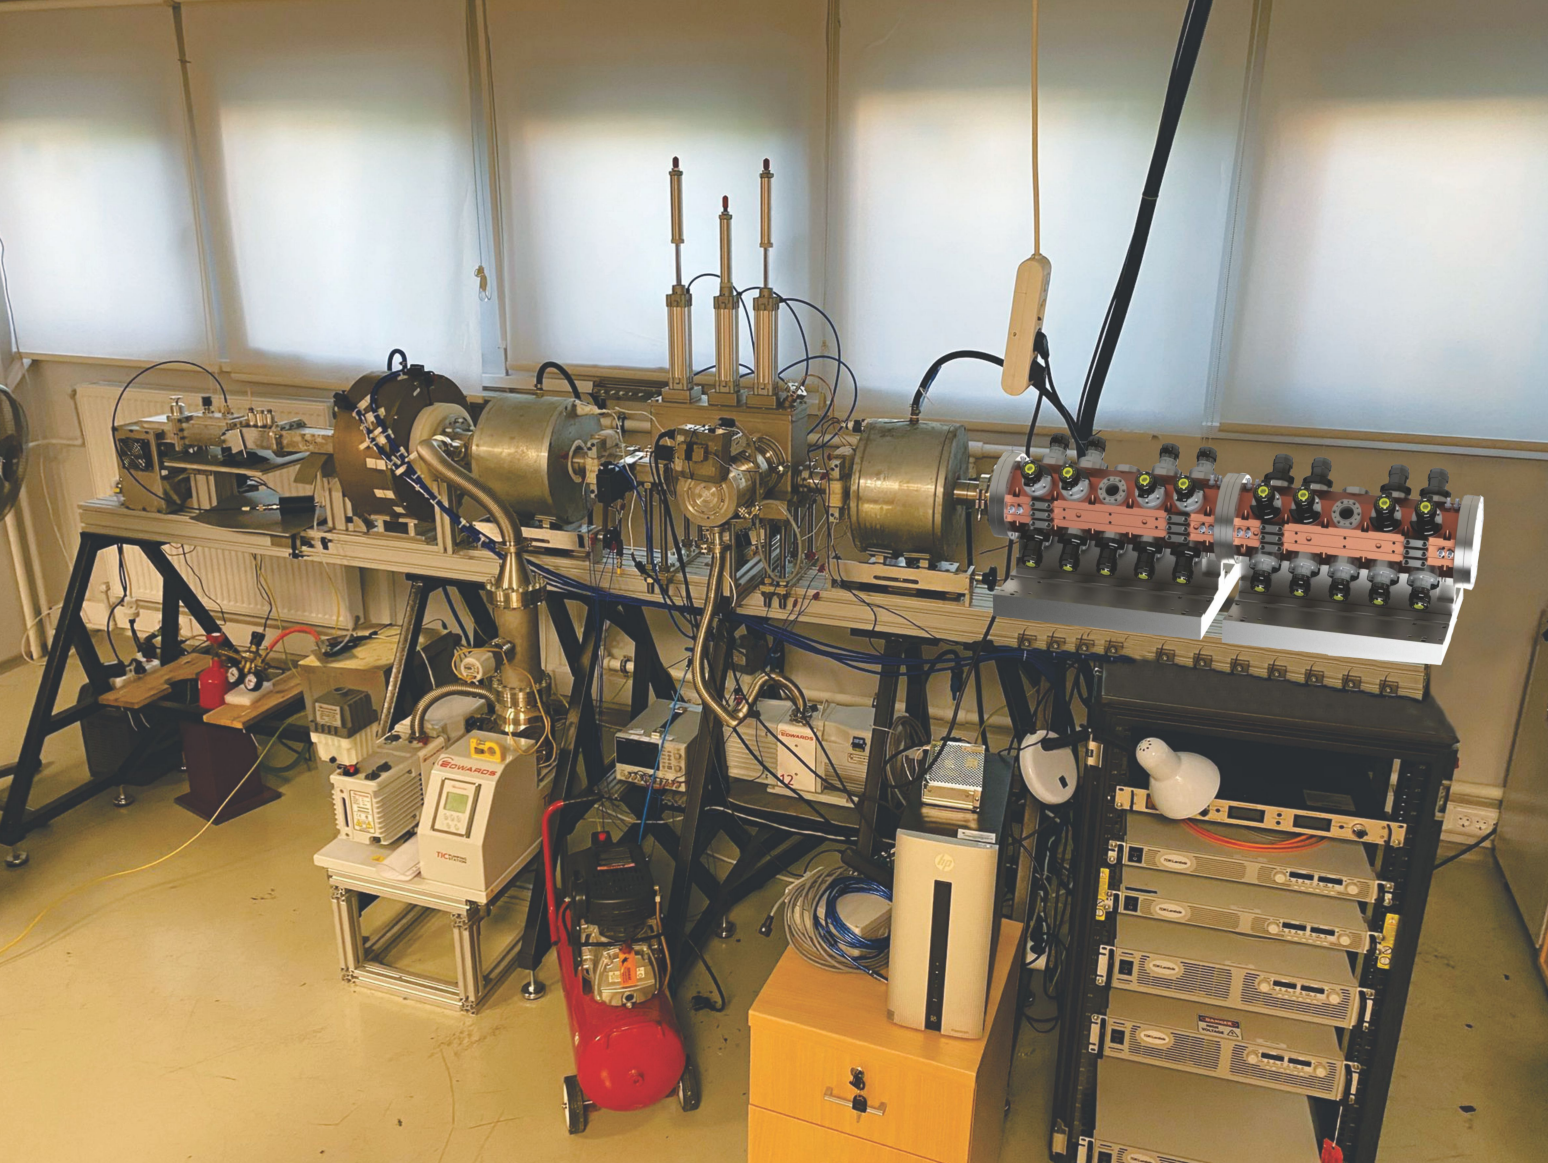
\includegraphics[width=.9\textwidth]{./figures/kahvelab_linac.png}
    \caption{A linear proton accelerator in KAHVELab \cite{kahvelab_linac}}
\end{figure}

\subsection{Acceleration Cavities} \label{sec:theory_cavities}
Radiofrequency (RF) cavities, also known as accelerating cavities or resonant cavities, are key components in particle accelerators. 
These cavities generate strong electromagnetic fields at specific frequencies to accelerate charged particles through clever engineering.

RF cavities are typically hollow metallic structures made of or coated with high-conductivity materials such as copper. 
They are designed to resonate at a specific frequency, which is determined by the size and shape of the cavity. 
The cavity is often cylindrical or spherical in shape, and its inner surface is polished to minimize energy losses through resistive heating.
The RF cavity is designed to be resonant, meaning that it naturally amplifies the electric fields at its resonant frequency. 
The resonant frequency is determined by the cavity's dimensions and the speed of light in the cavity material.

To achieve efficient energy transfer to the particles, the RF cavity is driven by an external RF power source operating at the resonant frequency. 
The power source supplies radiofrequency energy to the cavity, which causes the electric fields inside the cavity to oscillate at the desired frequency. 
These oscillating fields then transfer energy to the passing particles, increasing their kinetic energy by pushing and pulling on the charged particles as they pass through the cavity. 

In addition to accelerating the particles, RF cavities are often designed to provide focusing forces. 
By carefully shaping the cavity and adjusting the electromagnetic fields, the particles can experience focusing effects as they pass through the cavity. 
This helps to maintain a tight and controlled beam. To ensure efficient acceleration, it is essential to maintain phase stability. 
This means that the particles should experience the strongest electric fields at the correct time during their passage through the cavity. 
Precise timing and synchronization of the RF power source with the particle beam are crucial to achieve phase stability and maximize energy transfer.
\begin{figure}[H]
    \centering
    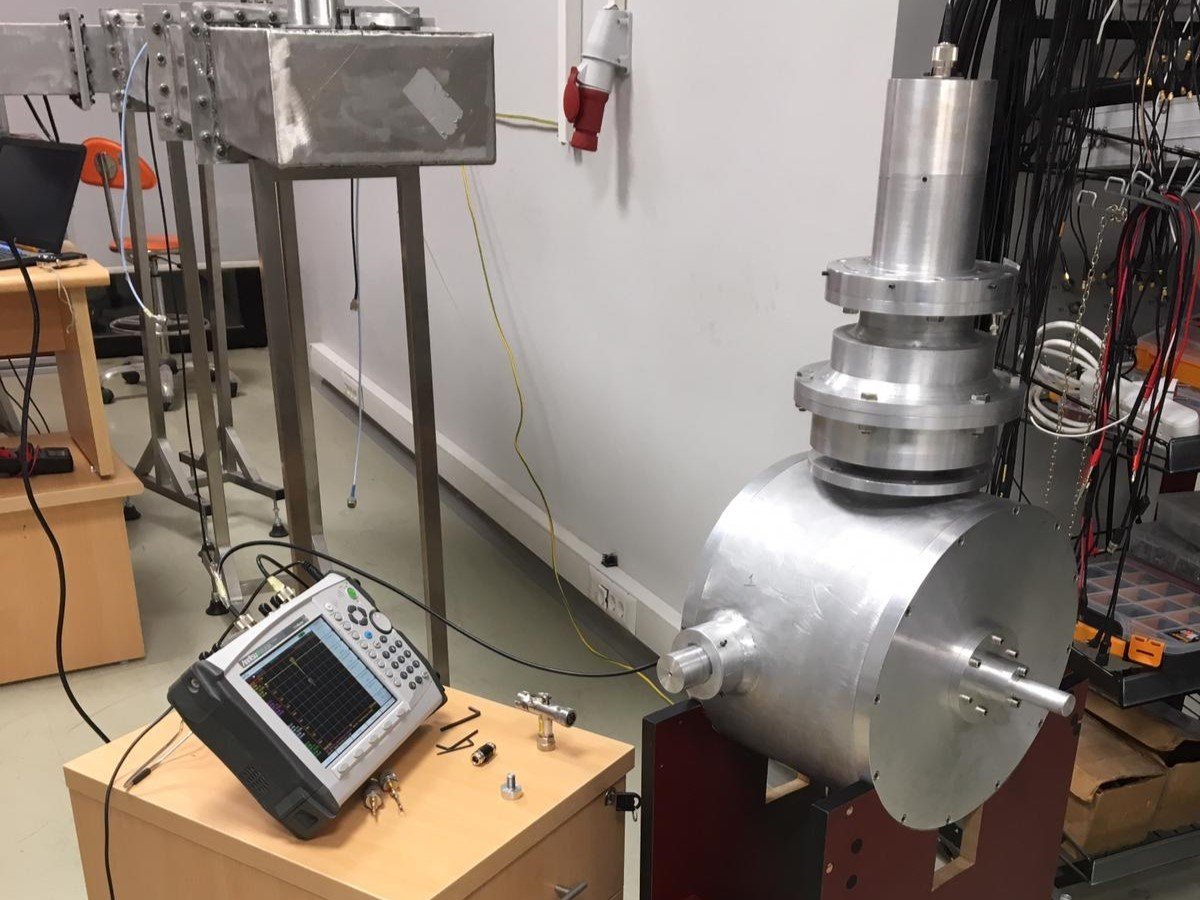
\includegraphics[width=.75\textwidth]{./figures/pill_box.jpeg}
    \caption{An RF cavity used in KAHVELab}
\end{figure}

\subsection{Bending Magnets}
Bending magnets, also known as dipole magnets, are fundamental components used in particle accelerators to control the trajectory of charged particles. 
They utilize the Ampere's Law to exert a magnetic field that interacts with the charged particles in the accelerator. 

According to the Lorentz Force Law (\fromsec{lorentz-force}), when a charged particle moves through a magnetic field, it experiences a force perpendicular to both its velocity 
vector and the magnetic field direction. This force causes the particle's trajectory to curve, resulting in a bending effect.


\subsection{Key Concepts}

\subsubsection{Resonance Frequency}
Resonance frequency is the frequency in which the electromagnetic fields form standing waves in a cavity.
It is determined by the physical dimensions and the speed of light in the cavity's medium. 
In a rectangular cavity for example, the resonance frequency can be calculated from \fromeq{f_r_rec}.
\begin{equation}
    f_{klm} = \frac{c}{2\pi \sqrt{\mu_r \epsilon_r}} \sqrt{(\frac{k}{w})^2 + (\frac{l}{u})^2 + (\frac{m}{v})^2}
    \label{eq:f_r_rec}
\end{equation}
where $w$, $u$, $v$ are the dimensions of the cavity, $\mu_r$ and $\epsilon_r$ are relative permability and permittivity of the cavity respectably.

\subsubsection{Bunch}
Bunch refers to a tightly grouped collection of charged particles, such as electrons or protons, that are accelerated and maintained close together within a particle accelerator.

\subsubsection{Phase Stability}
Phase stability refers to the preservation of the timing relationship between particles and fields within an accelerator. 
It ensures that the phases of various electromagnetic fields or particles remain synchronized, 
which is crucial for achieving efficient particle acceleration. 
Maintaining phase stability is essential to prevent particles from becoming out of phase as they travel through accelerator structures, 
ensuring that they receive the correct energy boosts and interact predictably with detectors. 
Deviations in phase stability can lead to particle loss and decreased beam quality.

\subsubsection{Phase Lag}
Phase lag refers to the time delay between the oscillations of two interacting waveforms or particles. 
It describes the difference in phase angles within their respective cycles, between two signals. 

\subsubsection{Shunt Impedance}
The shunt impedance of an RF accelerator is a measure of the efficiency 
at which the accelerator can transform the supplied RF power into acceleration.
It is defined as
\begin{equation} \label{eq:shunt}
    Z_s = \frac{V_{acc}^2}{P_{diss}}
\end{equation}
where $V_{acc}$ is the accelerating potential in which the particle is subjected to, 
$P_{diss}$ is the power dissipated on the cavity walls. 
An example \textit{shunt impedance} calculation can be found in \fromsec{cavity_of_a_rhodotron}.


\subsection{Rhodotron Accelerator} \label{sec:theory_rhodo}

Rhodotron Accelerator is a type of particle accelerator that was proposed by \textit{Jacques POTTIER} in 1989 \cite{rhodo_pottier}. 
First prototype was built at CEA Saclay later in 1992 \cite{rhodo_prototype}. It is named after the greek word for rose, \textit{rhodos}, due to the shape of the design \cite{rhodos}.

The design of a rhodotron mainly consists of a coaxial cylindrical RF cavity and bending magnets surrounding it. RF cavity is fed by an external RF source, accelerating the electrons entering from an attached electron injector.


\subsubsection{Acceleration cycle of Rhodotron}

Electrons undergo four different stages inside the accelerator. 
They are accelerated between the cylinderical plates and are shielded from the changing RF field while inside the inner cylinder and outside the cavity. 

\begin{description}
    \item[First acceleration] Electrons in the rhodotron cavity are accelerated by the electric field created between two coaxial cylinders, towards the inner cylinder when they are ejected into the cavity. (\fromfig{rhod_cycle_1})
    \item[Inner shielding] While inside the inner cylinder, the cylinder acts as a faraday cage and shields the electrons inside while the electric field is being reversed. (\fromfig{rhod_cycle_2})
    \item[Second acceleration] Once the electrons leave the inner cylinder, they accelerate towards the outer cylinder by the reversed electric field until they leave the cavity. (\fromfig{rhod_cycle_3})
    \item[Recirculating Magnets] After leaving the cavity, an electromagnet placed in their path steers the electrons back into the cavity in which time the electric field changes the direction again. (\fromfig{rhod_cycle_4})
\end{description}

This cycle can be repeated as long as real world constraints such as; placements and dimensions of the electromagnets, power requirements due to increasing magnetic field in order for sharper turns, can be overcomed.
After the desired amount of cycles, also called passes, has been completed, the electrons exit the accelerator.

This process is explained further in the \fromfigf{rhod_cycle_1}{rhod_cycle_2}{rhod_cycle_3}{rhod_cycle_4} where $T$ is the period of the electric field.

\subsubsection{Cavity of a Rhodotron} \label{sec:cavity_of_a_rhodotron}

Coaxial design of the cavity concentrates the electric field, while the magnetic field diminishes in the middle of the cylinders. 
Therefore the electrons are injected and accelerated in the plane of zero magnetic field where the electric field is strongest. (\fromfig{rhodo_cavity_field_dist})

\begin{figure}[H]
    \captionsetup[subfigure]{justification=centering}
    \captionsetup{justification=centering}
    \centering
    \begin{subfigure}{0.45\textwidth}
        \centering
        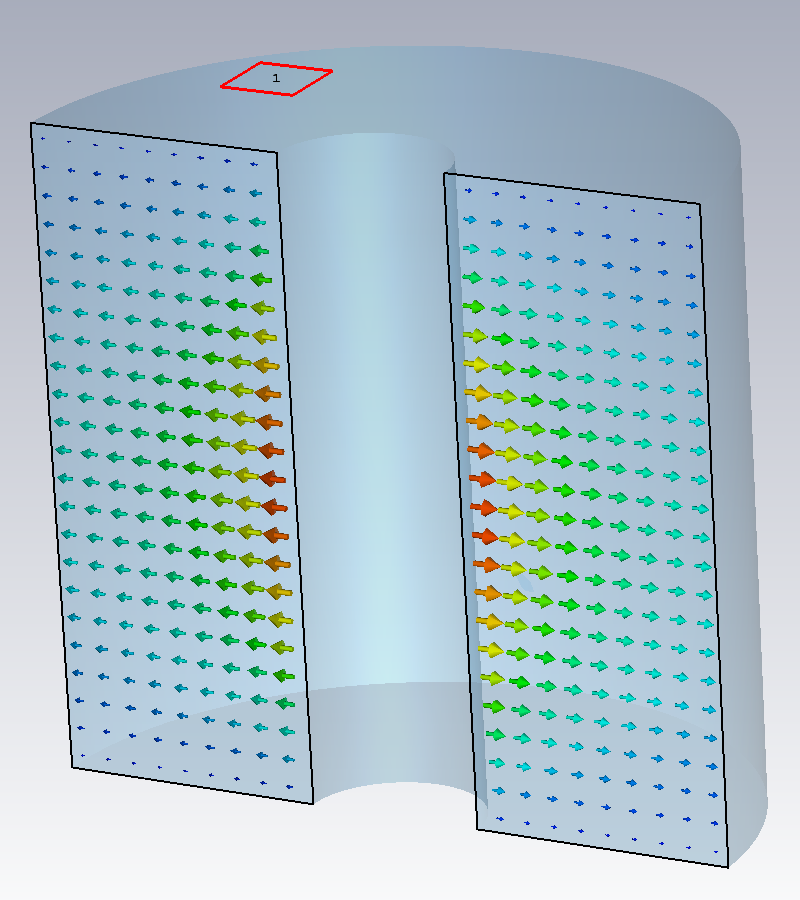
\includegraphics[width=\linewidth]{./figures/cst/cavity_E_field_dist.png}
        \caption*{$\vecthreeBF{E}$ field.}
    \end{subfigure}
    \begin{subfigure}{0.45\textwidth}
        \centering
        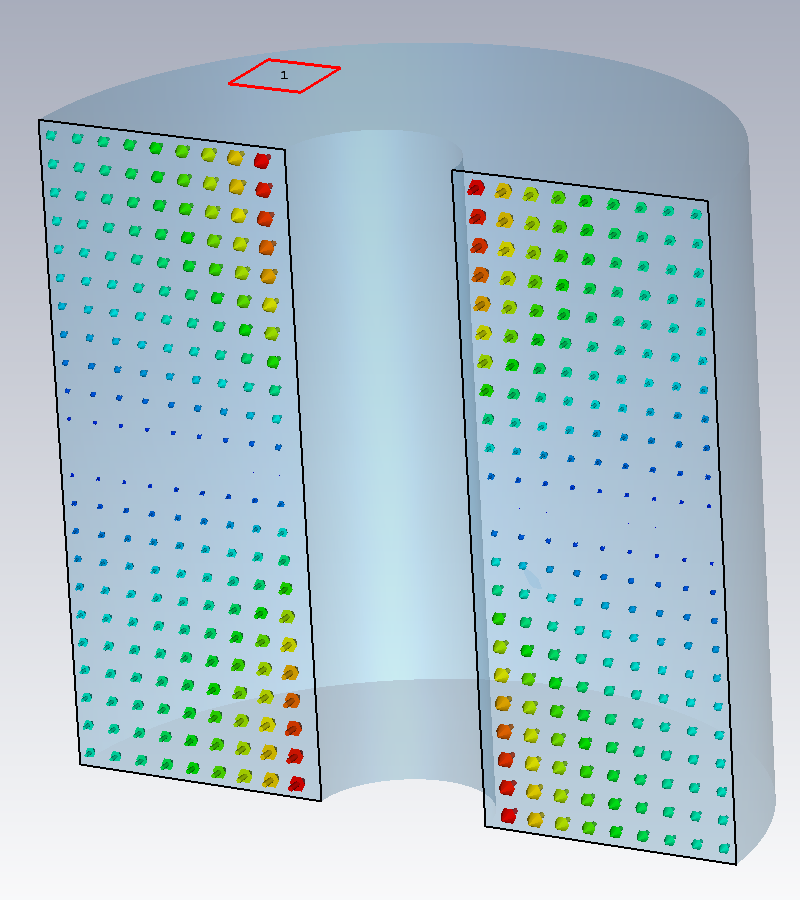
\includegraphics[width=\linewidth]{./figures/cst/cavity_B_field_dist.png}
        \caption*{$\vecthreeBF{B}$ field.}
    \end{subfigure}
    \caption{$\vecthreeBF{E}$ and $\vecthreeBF{B}$ eigenmode field distributions inside a coaxial cavity.}
    \label{fig:rhodo_cavity_field_dist}
\end{figure}
For a cavity defined by the volume between two coaxial cylinders of equal lengths ($h$) with radii of $R_1$ and $R_2$, where $R_1 < R_2$, located at the origin (\fromfig{int_curve}),
first eigenmode solution of the $E$ and $B$ fields are \cite{rhodo_pottier}
\begin{eqnarray}
    E &=& \frac{E_0}{r} \cos(\frac{\pi z}{h}) \sin(\omega t + \phi) \\
    B &=& \frac{B_0}{r} \sin(\frac{\pi z}{h}) \cos(\omega t + \phi)
\end{eqnarray}
where $\omega=2\pi f$, $f$ is the resonance frequency.

\begin{figure}[H]
    \centering
    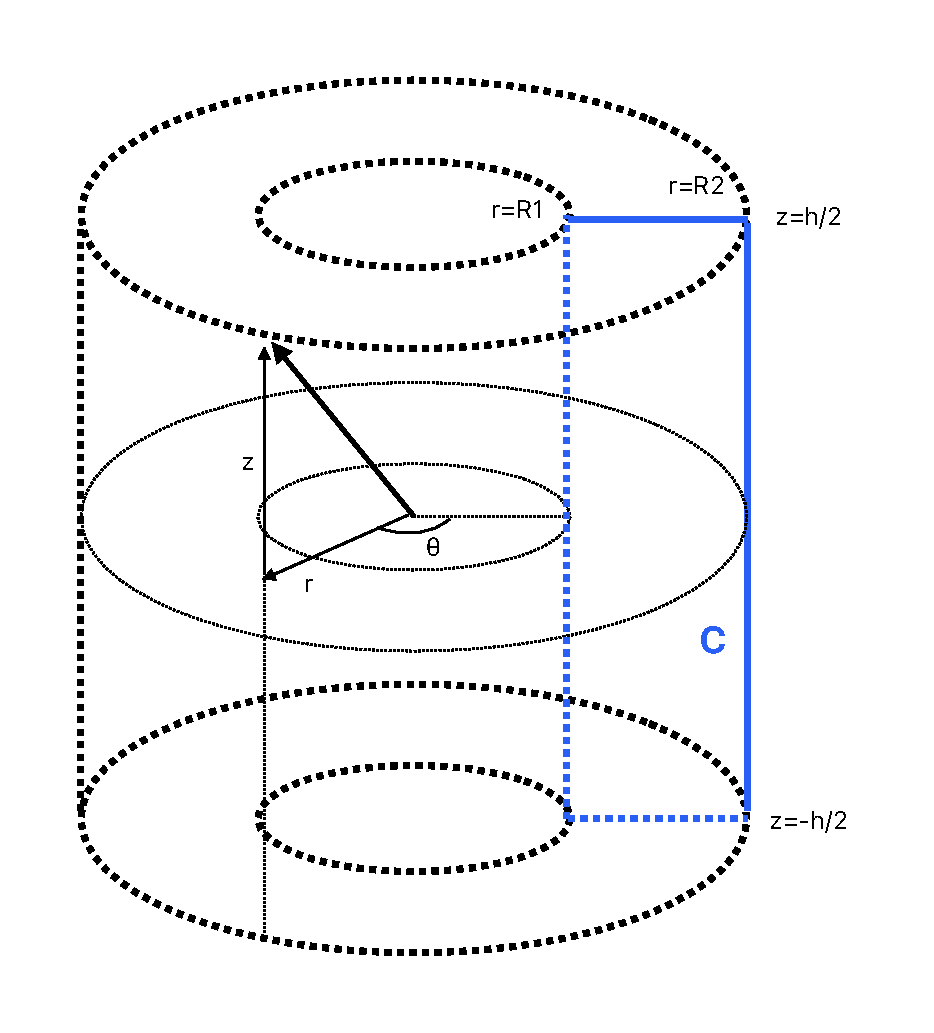
\includegraphics[width=.6\textwidth]{./figures/illustrations/rhodo_integral_curve.pdf}
    \caption{Illustration of a simple coaxial cavity with the curve \textbf{C} in \fromeq{p_diss_C_curve}}
    \label{fig:int_curve}
\end{figure}
Because acceleration potential is located on the $z=0$ plane and $\vecthreeBF{E} \parallel \hat{r}$, $V_{acc}$ can be found by the following equation:
\begin{eqnarray} 
    V_{acc} &=& 2 \int_{R_1}^{R_2} |E|^2 dr \\
            &=& 2 E_0 \int_{R_1}^{R_2} \frac{dr}{r} \\
            &=& 2 E_0 \ln(\frac{R_2}{R_1}) \label{eq:v_acc}
\end{eqnarray}
Dissipated power $P_{diss}$, on the other hand, can be calculated as follows \cite{rf}:
\begin{eqnarray} 
    P_{diss} &=& \frac{1}{2} \int \int \rho_s | H_{||} |^2 dA \nonumber \\
             &=& \frac{\rho_s}{2\mu_0^2} \int_0^{2\pi} \int_C | B_{||} |^2 r ds d\theta \label{eq:p_diss_C_curve}
\end{eqnarray}
where $\rho_s$ is the areal skin resistivity ( $\rho_s \approx 2.51 \times 10^{-7} f^{1/2}$ for copper \cite{rhodo_pottier} ), $B=\mu H$, $\mu$ is permeability, $\mu_0$ is the vacuum permability. 
Integral curve \textbf{C} is defined as the circumference of cylindrically symmetrical cross sectional area of the cavity (\fromfig{int_curve}).
This curve can be seperated to its line components and total power dissipation of this curve, $P_C$ will be equal to sum of the power dissipated in these lines.
Since $\vecthreeBF{B}$ is always parallel to the surface we can use $\vecthreeBF{B}$ directly:
\begin{eqnarray}
    P_{diss} &=& \frac{\rho_s}{2\mu_0^2} \int_0^{2\pi} (
                   2\int_{0}^{\frac{h}{2}} |B|^2 r dz \Big|_{r=R_1}
                 + 2\int_{0}^{\frac{h}{2}} |B|^2 r dz \Big|_{r=R_2} 
                 + 2\int_{R_1}^{R_2} |B|^2 r dr \Big|_{z=\frac{h}{2}})d\theta \nonumber\\
             %&=& \frac{\rho_s B_0^2 \cos^2(\omega t + \phi)}{2\mu_0^2} \int_0^{2\pi} 
             &=& \frac{\rho_s}{2\mu_0^2} \int_0^{2\pi} (2I_A + 2I_B + 2I_C)d\theta 
                 = \frac{2\rho_s \pi}{\mu_0^2}(I_A + I_B + I_C)
\end{eqnarray}
\begin{eqnarray}
    I_A = \int_{0}^{\frac{h}{2}} |B|^2 r dz \Big|_{r=R_1} &=& B_0^2 \frac{h}{4R_1} \\
    I_B = \int_{0}^{\frac{h}{2}} |B|^2 r dz \Big|_{r=R_2} &=& B_0^2 \frac{h}{4R_2} \\
    I_C = \int_{R_1}^{R_2} |B|^2 r dr \Big|_{z=\frac{h}{2}} &=& B_0^2 \ln(\frac{R_2}{R_1})
\end{eqnarray}
inserting $H_0=B_0/\mu_0$, finally we have the dissipated power:
\begin{equation} \label{eq:p_diss}
    P_{diss} = \rho_s \pi H_o ( \frac{h}{2R_1} + \frac{h}{2R_2} + 2\ln(\frac{R_2}{R_1}) )
\end{equation}
Therefore, from \fromeq{shunt}, using \fromeqs{v_acc}{p_diss} also $E_0/H_0 = Z_0 \approx 120 \pi$:
\begin{eqnarray}
    Z_s &=& \frac{4E_0^2}{H_0^2 \pi \rho_s} \frac{ \ln^2(\frac{R_2}{R_1})}{(\frac{h}{2R_1} + \frac{h}{2R_2} + 2 \ln(\frac{R_2}{R_1}))} \\
        &=& \frac{8 \pi 60^2}{\rho_s} \frac{ \ln^2(\frac{R_2}{R_1})}{(\frac{h}{4}(\frac{1}{R_1} + \frac{1}{R_2}) + \ln(\frac{R_2}{R_1}))}
\end{eqnarray}
where, time dependencies have been removed from $\vecthreeBF{E}$ and $\vecthreeBF{B}$ 
and the maximum values for $V_{acc}$ and $P_{diss}$ have been used. 
However, particles do not interact with constant $\vecthreeBF{E}$ field during acceleration. 
Therefore, a more useful parameter called \textit{effective shunt impedance} can be defined:
\begin{equation}
    Z_{se} = Z_s T^2
\end{equation}
where $T$ is the \textit{transit time factor}, a correctional coefficent that contain the changing field effects during acceleration.
For a relativistic electron crossing the axis at time 0, $T$ can be found by \cite{rhodo_pottier}:
\begin{eqnarray}
    T &=& \frac{S_i(\frac{2 \pi R_2}{\lambda}) - S_i(\frac{2 \pi R_1}{\lambda})}{\ln(\frac{R_2}{R_1})} \\
    S_i(\theta) &=& \int_0^{\theta} \frac{\sin(x)}{x} dx
\end{eqnarray}
for a relativistic electron crossing the axis at $2\pi f t_0 = \phi$ on the other hand, $T$ needs to be multiplied by $\cos(\phi)$:
\begin{equation}
    T(\phi) = T \cos(\phi)
\end{equation} 
Putting all these calculations together, energy gain of a relativistic electron, passing the origin at $\phi / \omega$ as calculated by \textit{J. Pottier} is \cite{rhodo_pottier}
\begin{eqnarray}
    \Delta E &=& q V_{acc}^{ef} \\
    \Delta E &=& q Z_{se}^{1/2}P_{diss}^{1/2} \cos(\phi)
\end{eqnarray}
where $ V_{acc}^{ef} = V_{acc} T(\phi)$ is the effective accelerating potential.
If $\Delta E$ is taken in \textit{MeV}, $Z_{se}$ in $M\Omega$ and $P_{diss}$ in \textit{MW}, this equality becomes
\begin{equation} \label{eq:W_gain_each_pass_pottier}
    \Delta E = Z_{se}^{1/2}P_{diss}^{1/2} \cos(\phi) \quad MeV
\end{equation}
With the expectation that the electrons will accelerate to speeds $\approx c$ after the first pass, a rhodotron cavity is designed so that the length of the path between successive passes is an integer multiple of $\lambda$, wavelength of the RF field ($l=p\lambda \label{eq:lpl}$).
This constraint helps with  phase stability and synchronization of the beam.

In the table below, optimized characteristics of a rhodotron cavity can be observed. 
\begin{figure}[H]
    \centering
    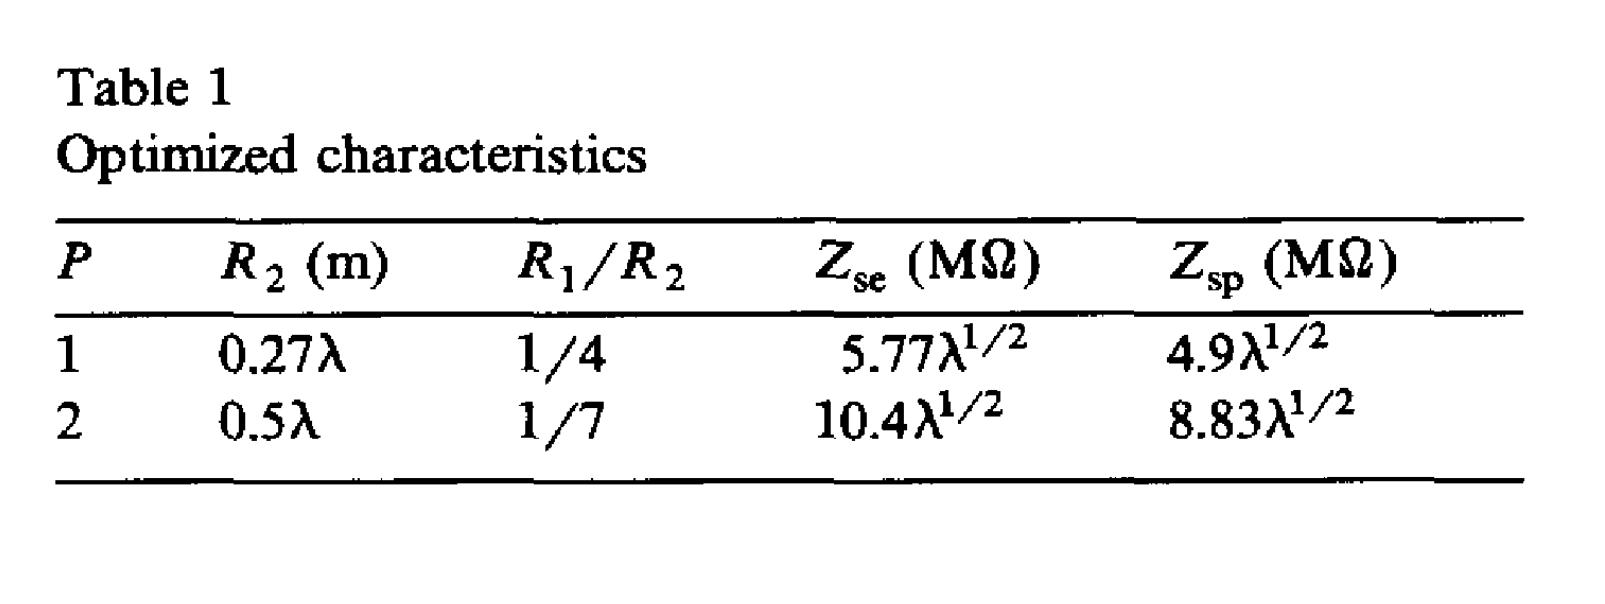
\includegraphics[width=.9\textwidth]{./figures/pottier_table1.png}
    \caption{Optimized characteristics of a rhodotron cavity \cite{rhodo_pottier}}
    \label{fig:pottier_table1}
\end{figure}
Here, $p$ is the integer multiplier in the equation ($l=p\lambda$) mentioned above, $R_1$ is the radius of the inner cylinder, $R_2$ is the radius of the outer cylinder, 
$Z_{se}$ is effective shunt empedance, $Z_{sp}$ is practical shunt empedance which was taken to be $0.85 Z_{se}$. Typically, phase lag $\phi$ is taken as $15^\circ$ \cite{rhodo_pottier}. 

Considering $Z_{sp} \propto \lambda^{1/2}$, \,\,\, $\Delta E \propto \lambda^{1/4}$, \,\,\,   $V \propto \lambda^3$, where $V$ is the volume of the cavity, implementing the $p=1$ design in \fromfig{pottier_table1} is much more space efficient.
\begin{figure}[H]
    \centering
    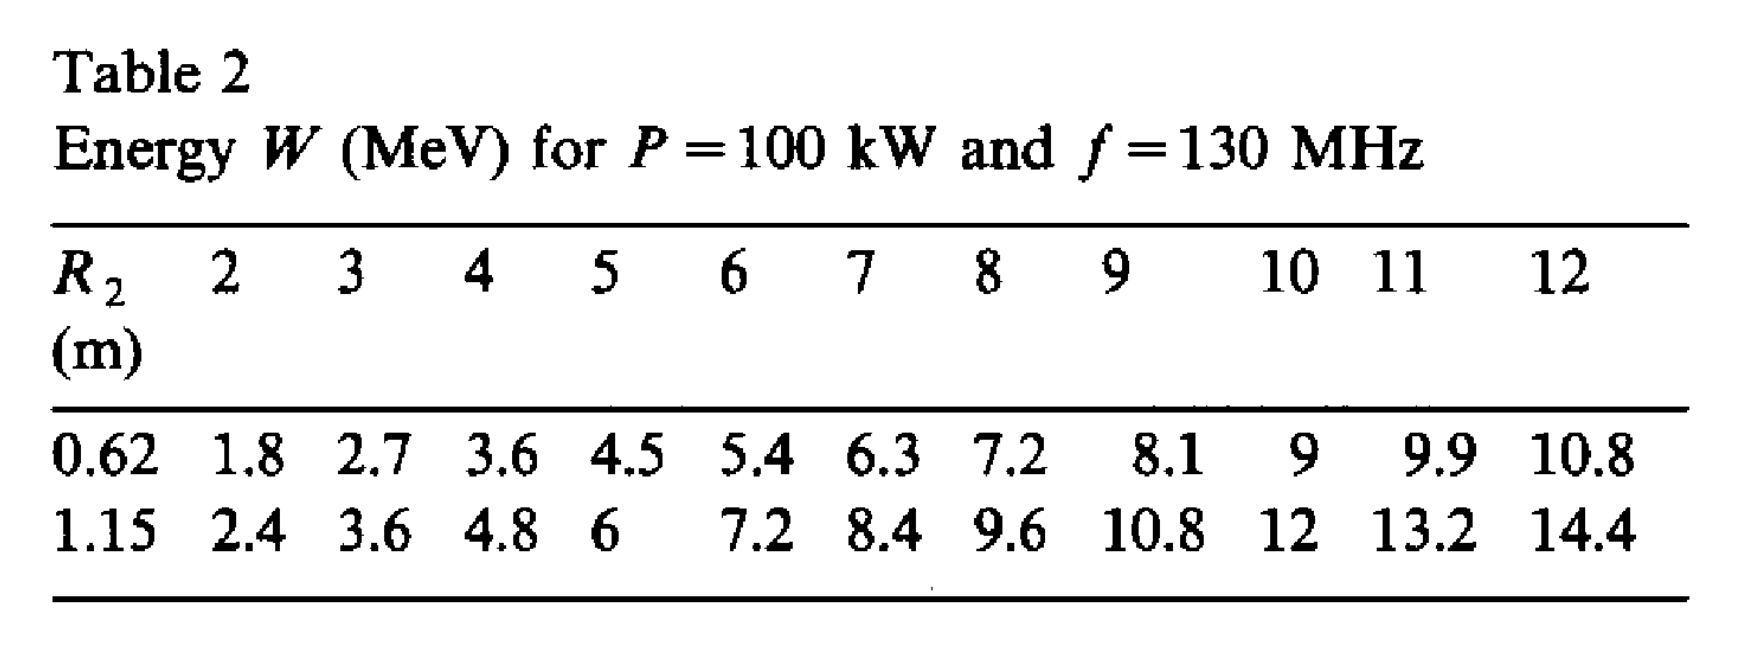
\includegraphics[width=.9\textwidth]{./figures/pottier_table2.png}
    \caption{Energy of a synchronous electron after each pass for both $p=1$ and $p=2$ \cite{rhodo_pottier}}
    \label{fig:pottier_table2}
\end{figure}
Total energy gain after $n$ passes, $\Delta E_n$, can then be found by \fromeq{W_gain_each_pass_pottier}, taking $\phi = 15^\circ$, $p=1$, i.e $R_2 = 0.27 \lambda$, $P$ in \textit{W}, $\lambda$ in \textit{m}.
\begin{equation}
    \label{eq:W_total_gain_pottier}
    \Delta E_n \approx 2.14 \lambda^{1/4} P^{1/2} n \quad keV
\end{equation}


\begin{figure}[H]
    \centering
    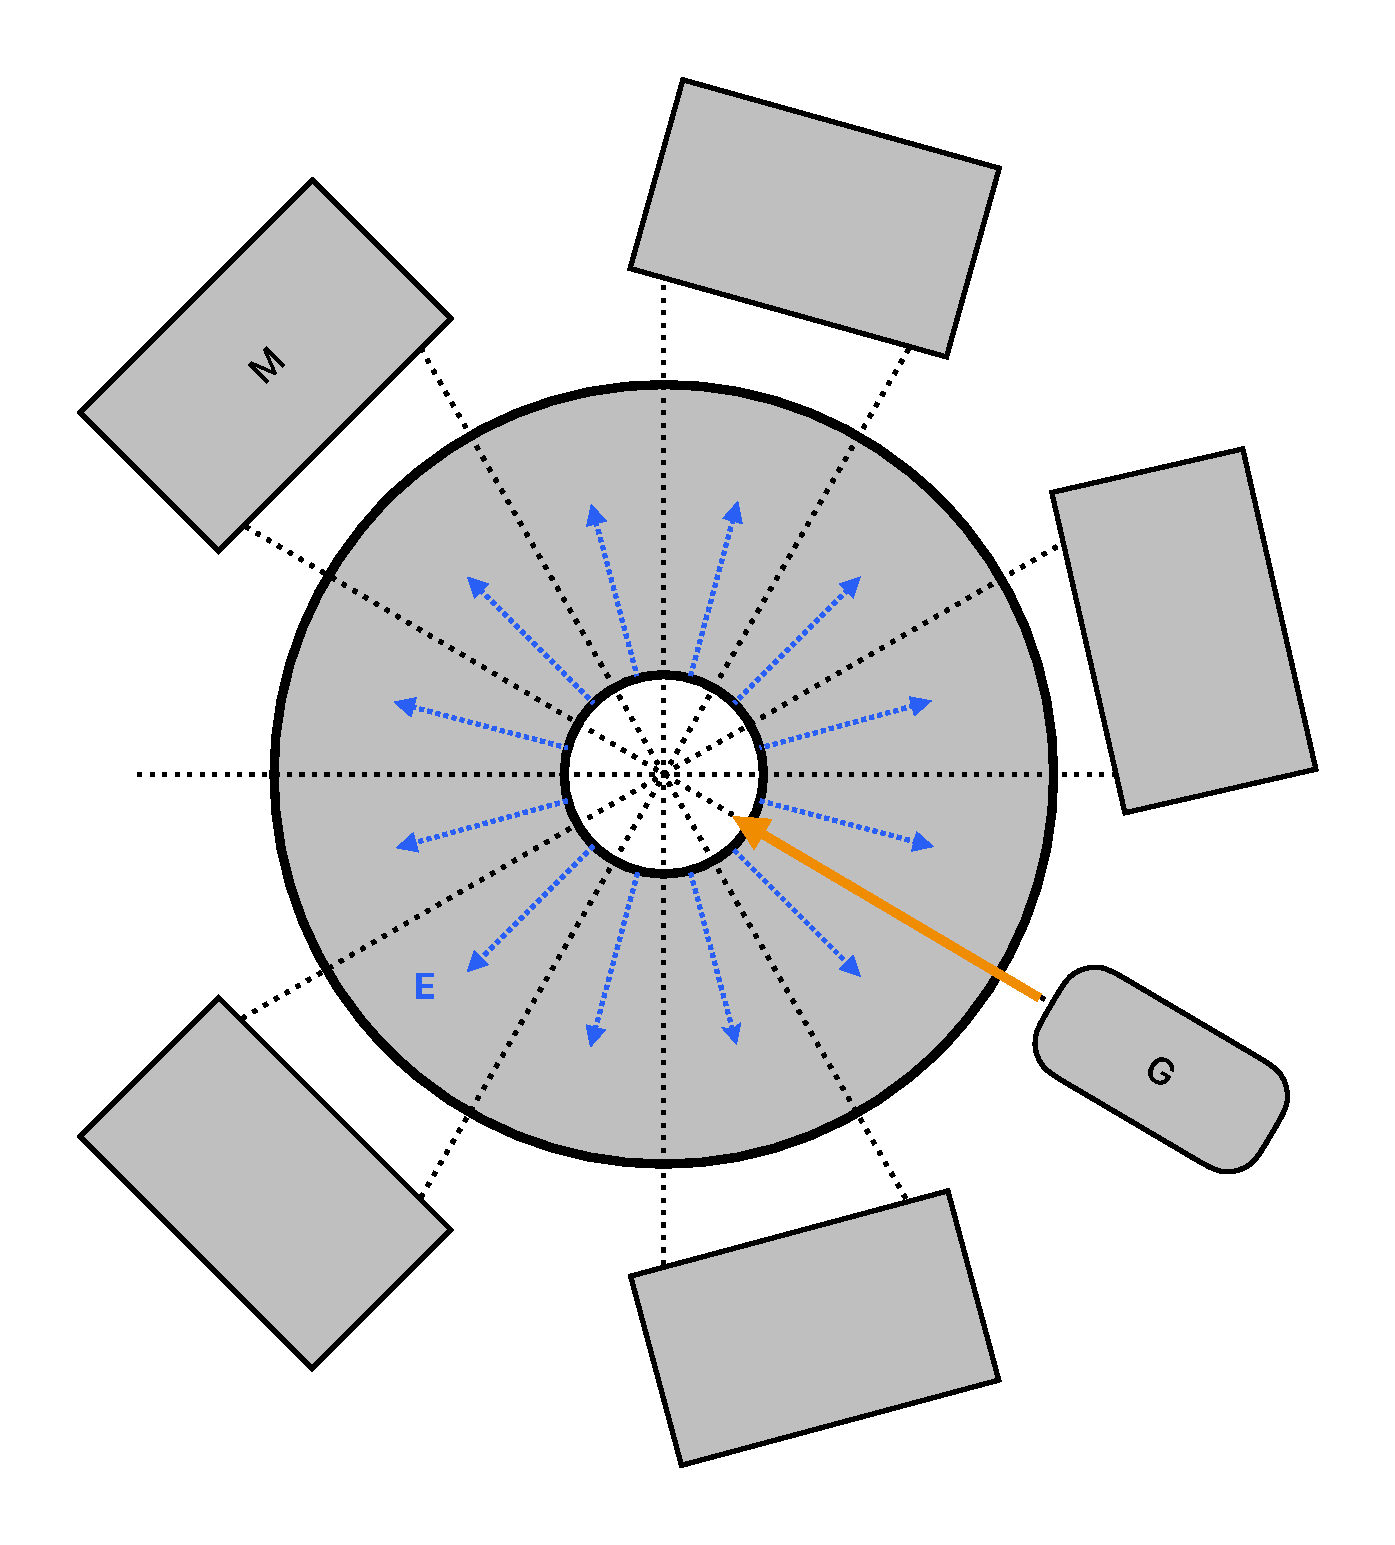
\includegraphics[width=\textwidth]{./figures/illustrations/rhod1.pdf}
    \caption{$[0, \frac{T}{4}]$ time frame of a rhodotron}
    \label{fig:rhod_cycle_1}
\end{figure}
\begin{figure}[H]
    \centering
    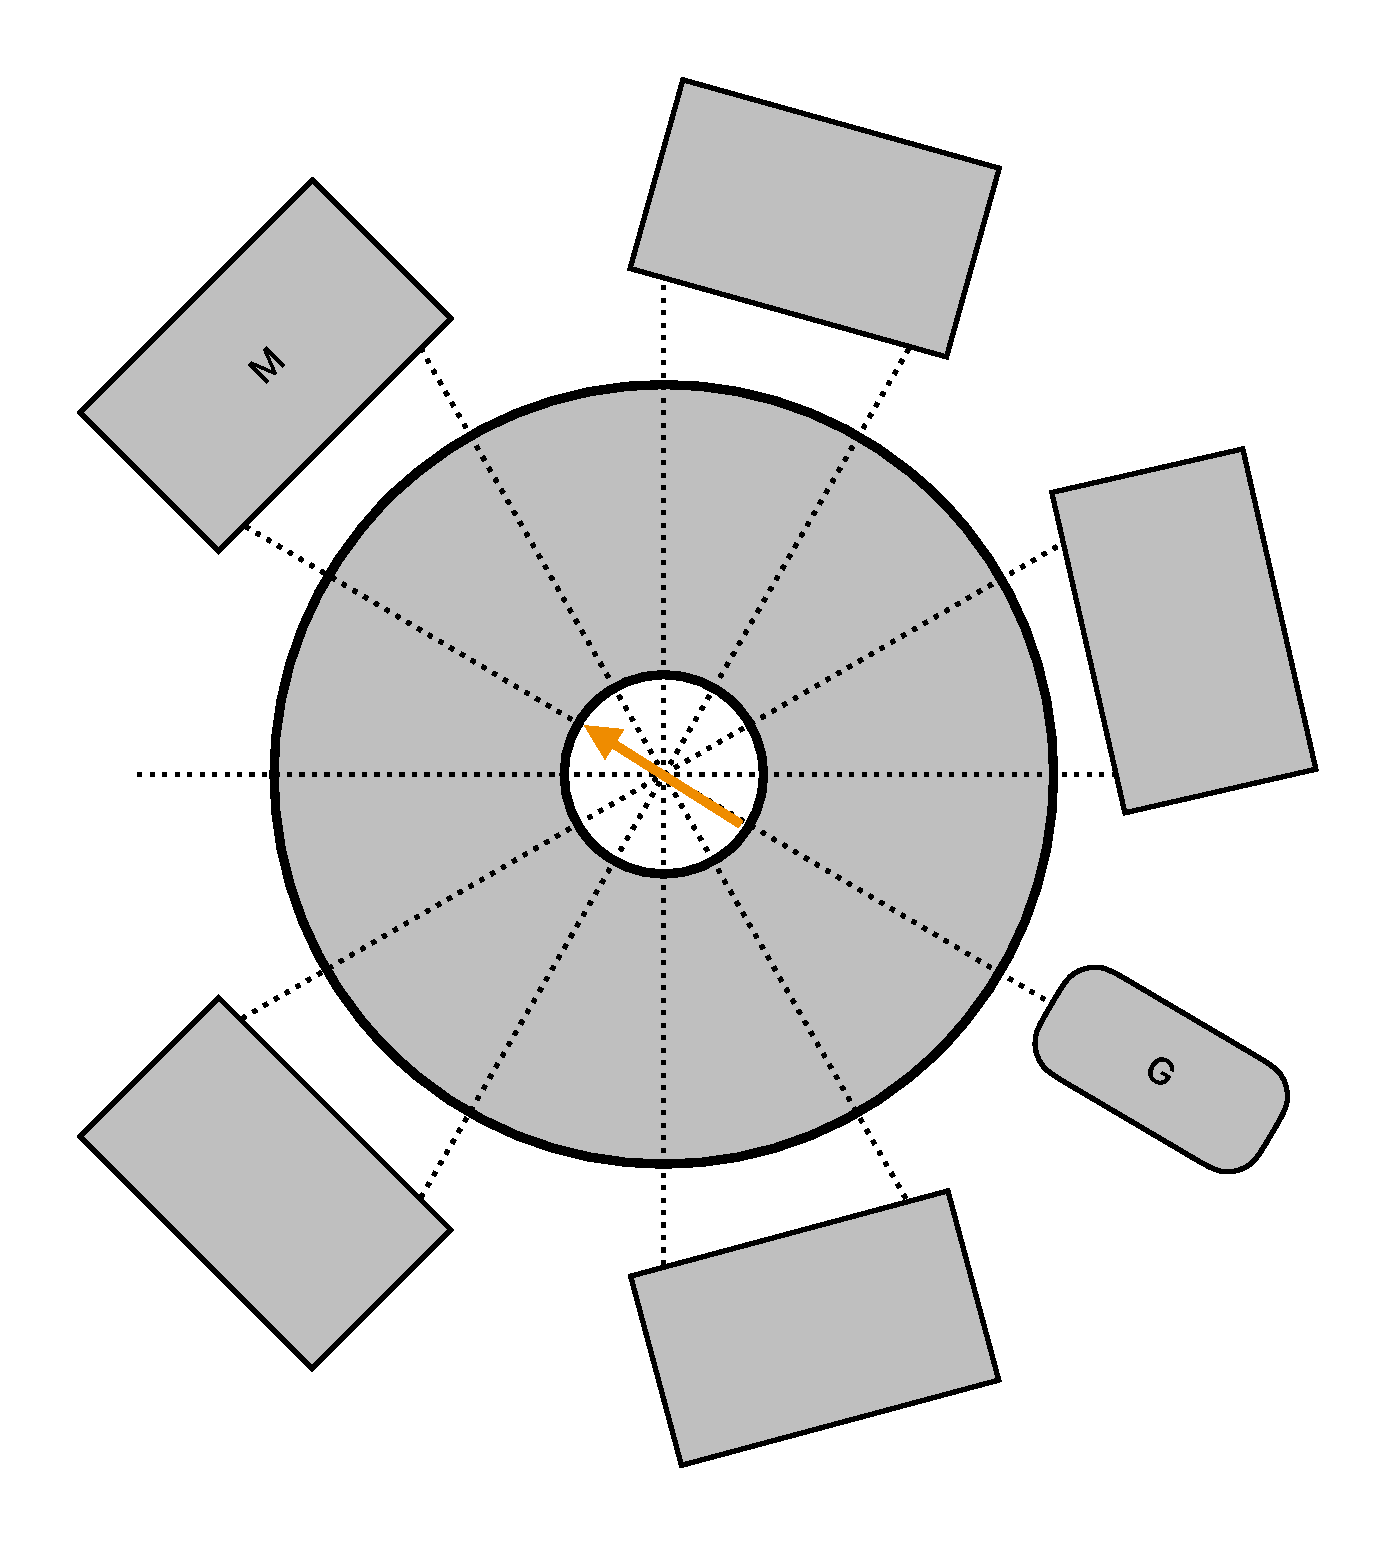
\includegraphics[width=\textwidth]{./figures/illustrations/rhod2.pdf}
    \caption{$[\frac{T}{4}, \frac{T}{2}]$ time frame of a rhodotron}
    \label{fig:rhod_cycle_2}
\end{figure}
\begin{figure}[H]
    \centering
    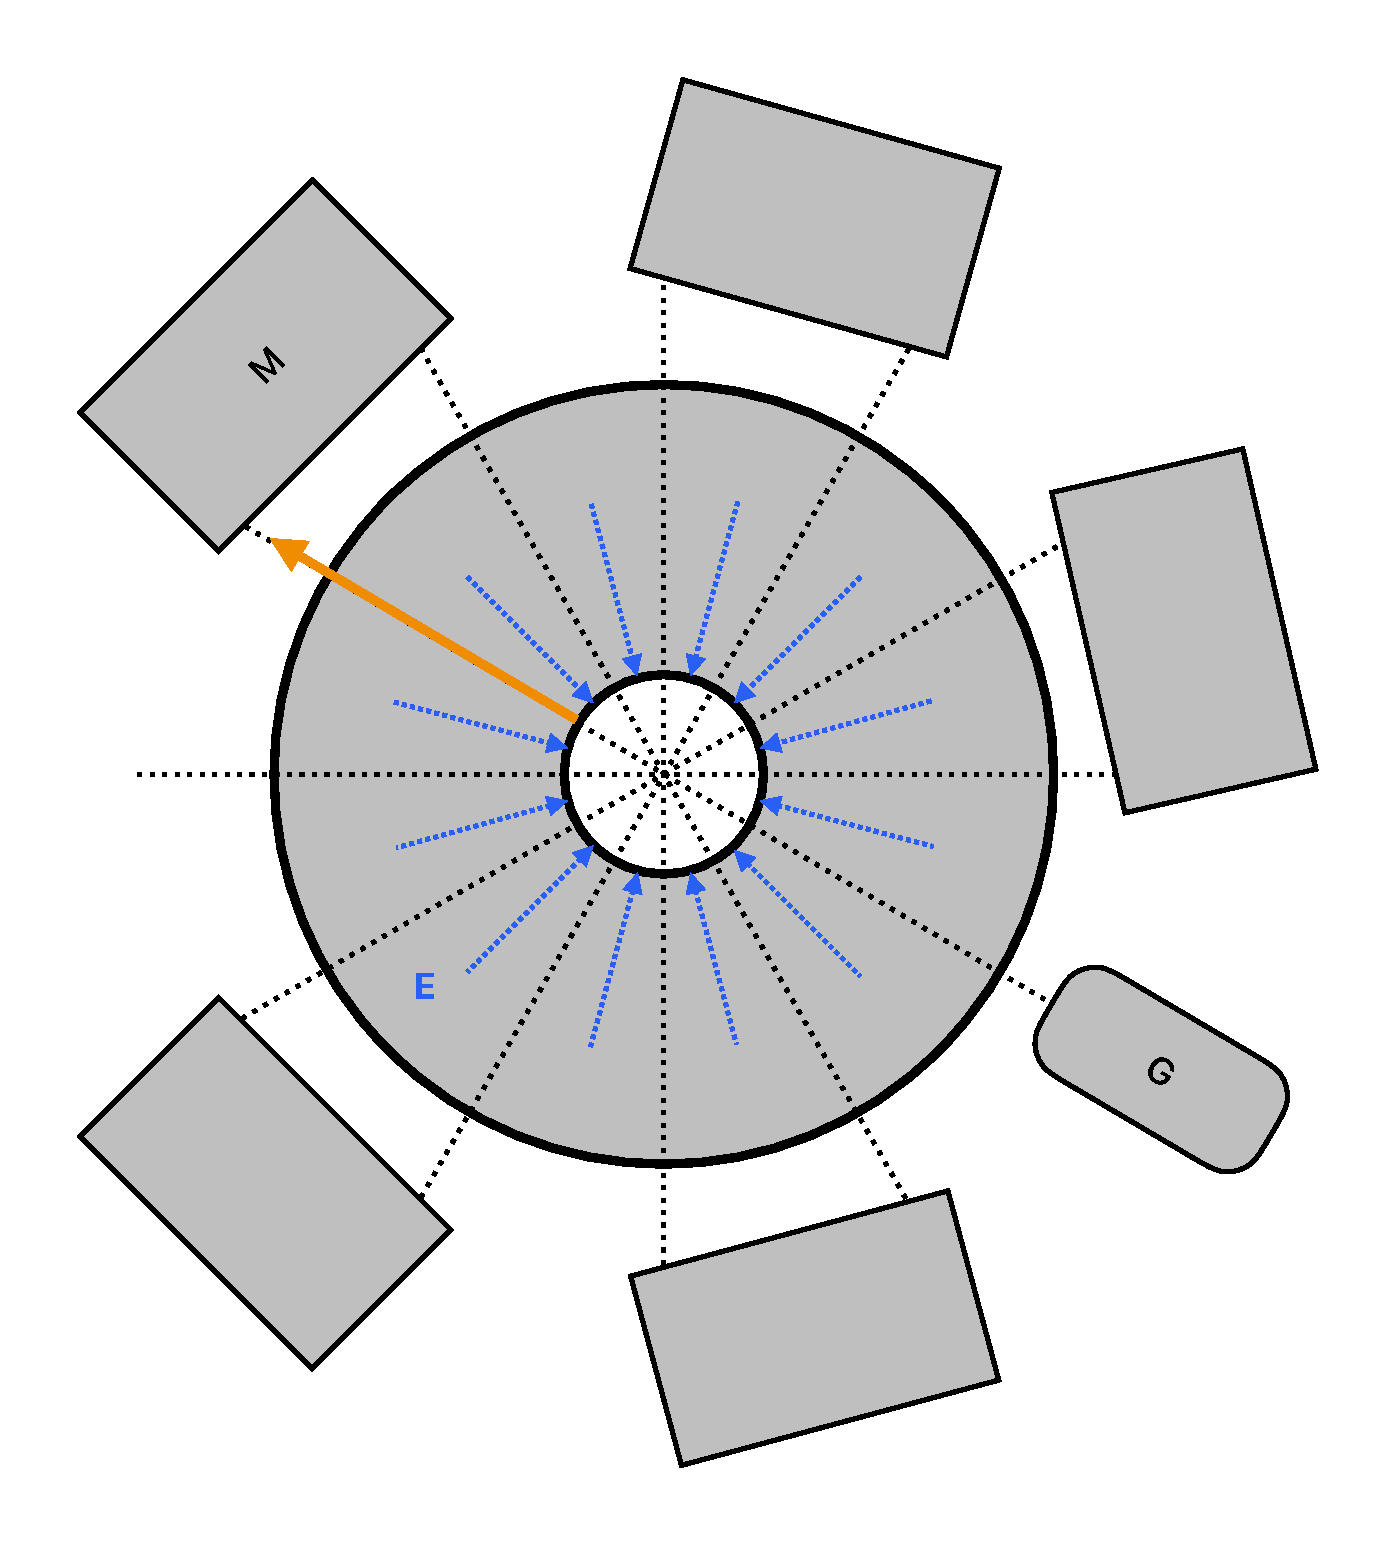
\includegraphics[width=\textwidth]{./figures/illustrations/rhod3.pdf}
    \caption{$[\frac{T}{2}, \frac{3T}{4}]$ time frame of a rhodotron}
    \label{fig:rhod_cycle_3}
\end{figure}
\begin{figure}[H]
    \centering
    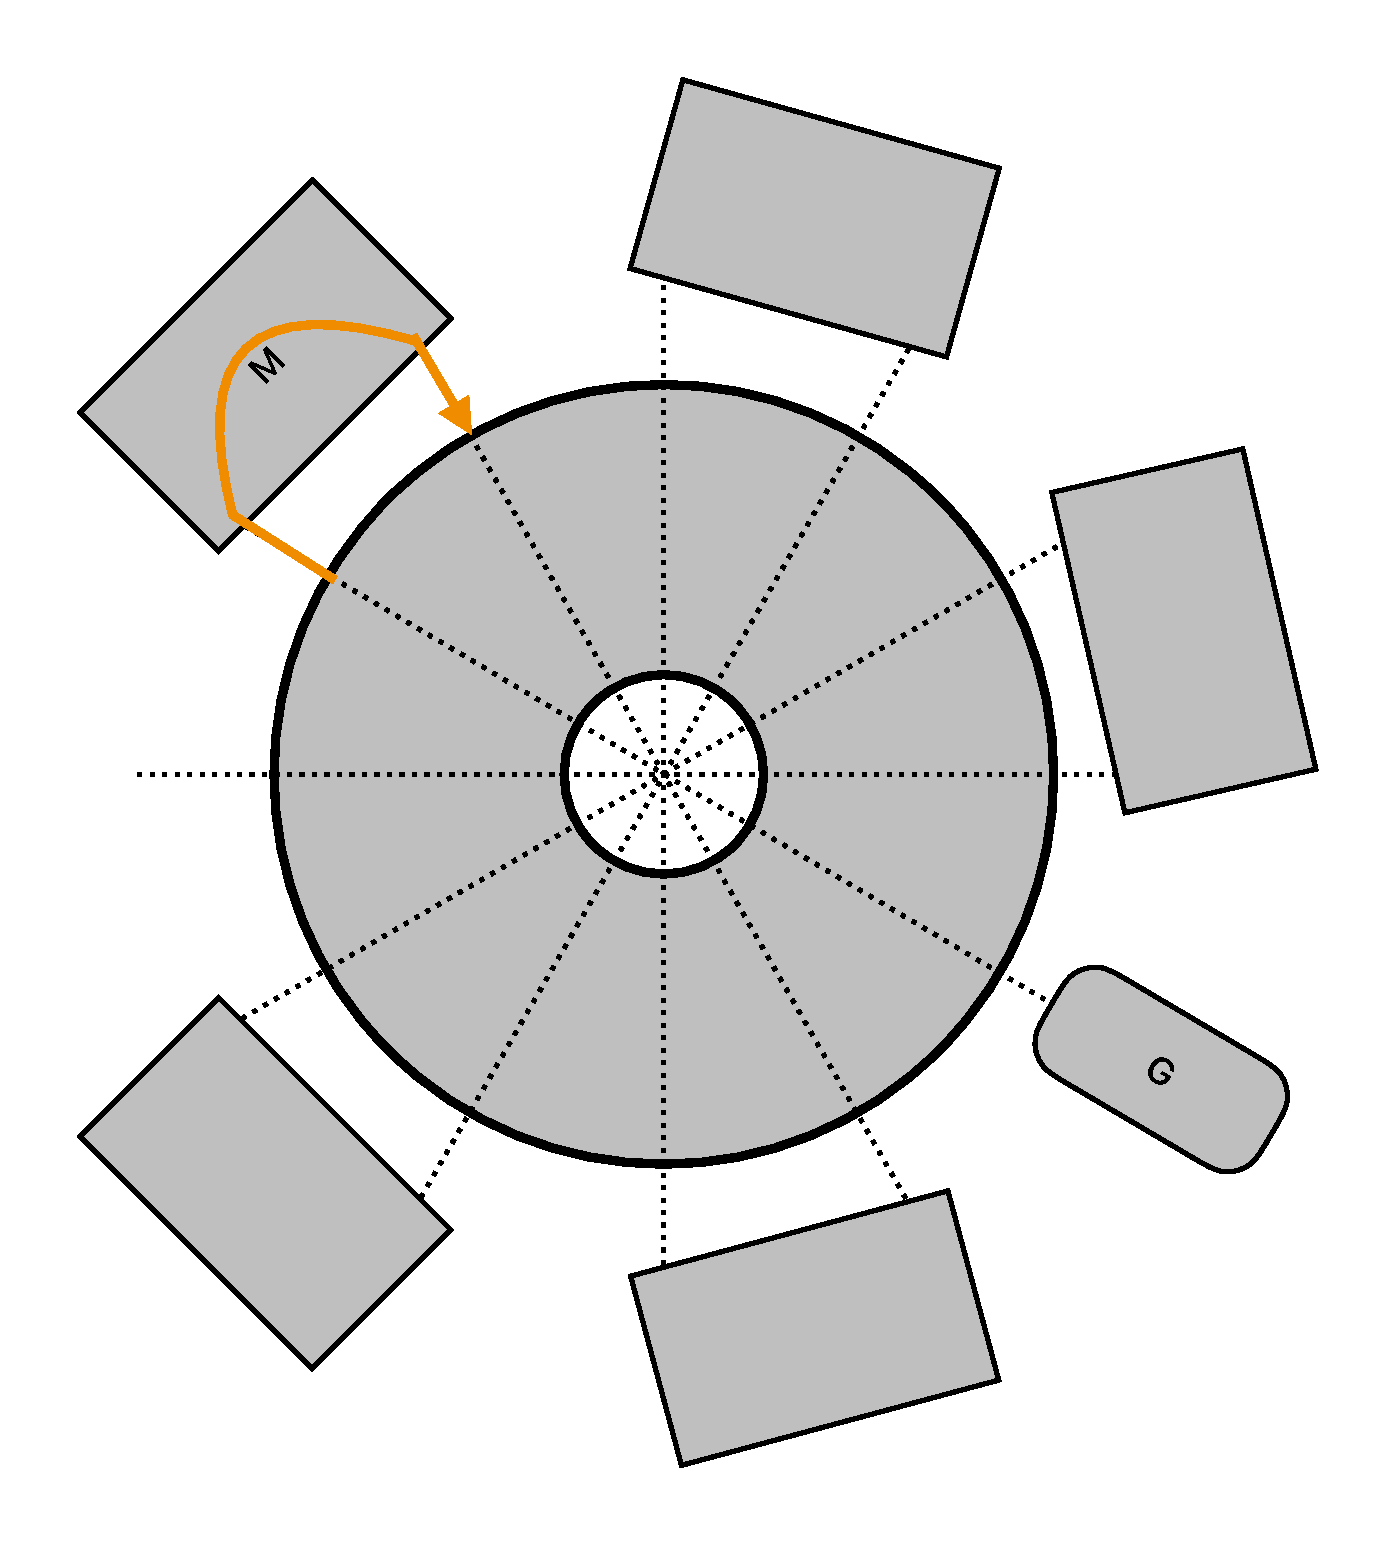
\includegraphics[width=\textwidth]{./figures/illustrations/rhod4.pdf}
    \caption{$[\frac{3T}{4}, T]$ time frame of a rhodotron}
    \label{fig:rhod_cycle_4}
\end{figure}





\section{Basic Concepts in Programming}

\subsection{Clock Cycle}

In programming, a clock cycle refers to a fundamental unit of time measurement used in computer systems. 
It represents the basic rhythm or timing mechanism of a computer's central processing unit (CPU) and is typically measured in terms of the CPU's clock speed, expressed in hertz (Hz).

A clock cycle represents one complete pulse or oscillation of the CPU's clock signal. 
It serves as a synchronization mechanism, coordinating the execution of instructions and the timing of various operations within the CPU.
Each clock cycle is associated with a specific duration, which is determined by the clock speed of the CPU.

The concept of clock cycles is often used when considering the performance and efficiency of algorithms and code. 
Since the execution time of instructions is influenced by the number of clock cycles required, minimizing the number of clock cycles needed for a program or algorithm can lead to faster and more efficient code execution.
Table below shows the amount of clock cycles required for some mathematical calculations in various processors.
\begin{figure}[h!]
    \centering
    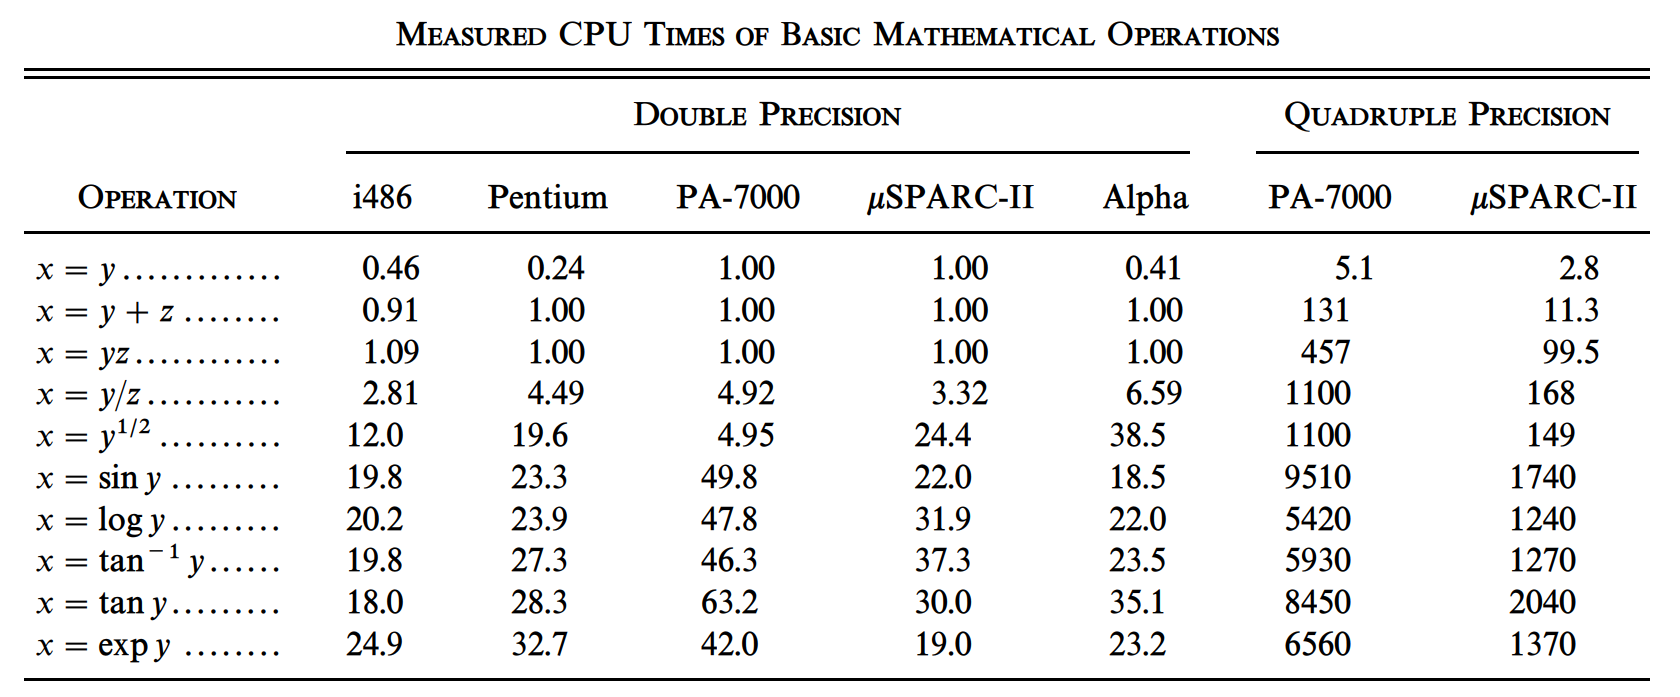
\includegraphics[width=.9\textwidth]{./figures/cpu_instruction_speed.png}
    \caption{Amount of clock cycle for mathematical operations in various processors. \cite{cpu_instruction_speed}}
\end{figure}
Note that \textit{division} is by far the most time consuming basic mathematical operation between addition, subtraction and multiplication.

Although not discussed in the following chapters, mathematical operations were reduced to addition, subtraction and multiplication when found to be possible while developing computationally intensive software in \fromch{simulation}.

\subsection{Concurrency}

Concurrency in programming refers to the ability of a program to execute multiple tasks or processes simultaneously. It allows different parts of a program to make progress independently, potentially improving performance, responsiveness, and resource utilization.

Concurrency in single core can be achieved by implementing clever scheduling of list of operations called \textit{threads}. This results in non-blocking execution of multiple threads, but only one thread would be executed at any given time. 
True concurrency on the other hand, can only be achieved by using multiple cores. Each core would be able to execute one thread at any time.

Programs that implement concurrency using multiple cores executes more operations per clock cycle. 
However, this does not directly lead to an improved performance due to the heavy burden of scheduling and managing multiple threads.

Threads utilize \textit{mutexes}, short for "mutual exclusion," 
to synchronize and manage access to shared resources 
in a multi-threaded or multi-process environment. 

\subsection{Object Oriented Programming}

Object-Oriented Programming (OOP) is a programming paradigm that revolves around the concept of objects. 
Definition called class serves as a blueprint that defines the structure and behavior of objects. 
Each object encapsulates both data, and the functions that manipulate that data. 
This encapsulation promotes modular code design and enhances data security by controlling access to the object's internal state. 

In OOP, \textit{inheritance} enables the creation of new classes based on existing ones, facilitating code reuse and hierarchy. 
\textit{Polymorphism} allows objects of different classes to be treated uniformly through a common interface, enhancing flexibility and extensibility. 
By providing abstraction, OOP simplifies complex systems by focusing on essential features and interactions, making software development more manageable, scalable, and maintainable.



\newpage

% START OF common_start_tools.tex

\chapter{TOOLS}

For the purpose of designing, enhancing, and optimizing particle accelerators, certain tools can be employed. 
The following sections will explore several of the software and algorithms that were put to use.

\section{Simulation}
A simulation software is a computer program or tool that enables the creation and execution of 
simulations to model and analyze real-world systems or processes. 
It allows users to replicate the behavior, interactions, and outcomes of the system or process under study, 
providing insights and predictions that can be valuable for decision-making, optimization, or understanding complex phenomena.

Simulation software provides a virtual environment where users can define the parameters,
variables, and rules of the system being simulated. The software then uses mathematical and physical models, 
algorithms, and computational techniques to simulate the behavior of the system over time.


% START OF available.tex

\section{Available Tools}

\subsection{Poisson Superfish}
Poisson Superfish is a software package developed by the \textit{Los Alamos National Laboratory} 
for the design and analysis of electromagnetic fields, particularly those related to particle accelerators and high-energy physics experiments \cite{poi-sup}.
It is commonly used in the field of accelerator physics to simulate and optimize the behavior of charged particle beams as they pass through various electromagnetic structures, such as cavities and magnets.


\subsection{CST Studio Suite}
CST Studio Suite is a powerful software package developed by \textit{Simulia} for electromagnetic simulation and analysis. It is widely used in various industries, including electronics, telecommunications, automotive, aerospace, and more, to design and optimize electromagnetic devices and systems. 
The software provides a comprehensive set of tools for simulating and analyzing the behavior of electromagnetic fields and their interactions with different materials, structures and charged particles.

\subsection{ROOT}
ROOT is a widely used open-source software framework developed by CERN (European Organization for Nuclear Research) for data analysis,
visualization, and storage in the field of high-energy physics, particularly in experiments conducted at particle accelerators 
like the Large Hadron Collider (LHC) \cite{root}. It has become an essential tool in particle physics research, 
and it is used by physicists around the world to analyze and interpret data.

\subsection{gnuplot}
GNUPLOT is a popular open-source software used for creating and visualizing data plots and graphs  \cite{gnuplot}. 
It is widely utilized in various fields, including scientific research, data analysis, engineering, and more, 
to represent and analyze data in a graphical format. 



\section{Algorithms}

\subsection{Leapfrog} \label{sec:leapfrog}
The Leapfrog method is a numerical method commonly used to solve ordinary differential equations (ODEs) that involve second-order time derivatives. Such an ODE is shown below:
\begin{equation}
    \ddot{x} = \derivS{x}{t} = f(x) \label{eq:second-order-ODE}
\end{equation}
\newline
The Leapfrog method is a variant of the finite difference method, and it approximates the solution of an ODE by discretizing both time and space. The method gets its name from the way it calculates the values of the solution at each time step, which resembles a "leapfrogging" motion. 
It is a simple and efficient algorithm that is often used in simulations of physical systems, such as celestial mechanics or molecular dynamics.
The idea is straight forward; in the time interval $\Delta t$, 
\begin{eqnarray}
    a(t_0) &=& f(x_0) \nonumber \\
    x(t_0 + \Delta t) &=& x(t_0) + v(t_0)\Delta t + a(t_0)\frac{\Delta t^2}{2} \label{eq:leapfrog_sync_x}\\
    v(t_0 + \Delta t) &=& v(t_0) + \{ a(t_0) + a(t_0 + \Delta t)\}\frac{\Delta t}{2}  \label{eq:leapfrog_sync_v}
\end{eqnarray}
For more stability, this version can be rearranged to what is called 'kick-drift-kick' form,
\begin{eqnarray} \label{eq:leapfrog}
    v(t_0 + \Delta t/2) &=& v(t_0) +  a(t_0)\frac{\Delta t}{2} \nonumber \\
    x(t_0 + \Delta t) &=& x(t_0) + v(t_0 + \Delta t/2)\Delta t \\
    v(t_0 + \Delta t) &=& v(t_0 + \Delta t/2) + a(t_0 + \Delta t)\frac{\Delta t}{2}  \nonumber
\end{eqnarray}
This version provides more time resolution to our calculation; however, it increases the number of calculations needed by about $50\%$.

\subsection{Runge Kutta} \label{sec:rungekutta}

The Runge-Kutta methods, named after the German mathematicians Carl Runge and Martin Wilhelm Kutta \cite{runge} \cite{kutta}, family of numerical methods
used to solve ordinary differential equations (ODEs) that are in the following form
\begin{equation} \label{eq:first-order-ODE}
    \parDeriv{y}{x} = f(x, y)
\end{equation}
The basic idea behind the Runge-Kutta method is to approximate the solution of an ODE by taking small steps and using a weighted average 
of function evaluations at different points within each step.
\begin{equation} \label{eq:general-rk}
    \begin{aligned}
        y_{n+1} = y_n + \delta x \sum_{i=1}^{m} b_i k_i
    \end{aligned}
    \qquad
    \begin{aligned}
        x_{n+1} = x_n + \delta x 
    \end{aligned}
\end{equation}
where 
\begin{eqnarray} \label{eq:general-rk-coef}
    k_i = f(x_n + c_i \delta x, y_n + \delta x \sum_{j = 1}^{i - 1}a_{ij}k_j)
\end{eqnarray}
These \fromeqs{general-rk}{general-rk-coef} define the family of methods. To specify a perticular method, order $m$, coefficients $a_{ij}$, $b_i$ and $c_i$ should be provided.
The coefficients of any Runge-Kutta method can be visualized by a tableau called $\textit{Butcher Tableau}$.
\begin{figure}[h!]
    \[ 
    \begin{array} 
        {c|cccc}
        0\\
        c_1 & a_{21} \\
        c_2 & a_{31} & a_{32}\\
        \vdots& & \cdots& \\
        c_m & a_{m1} & a_{m2} & \cdots & a_{m,m-1}\\
        \hline
        & b_1 & b_2 &\cdots & b_m
    \end{array}
    \]
    \caption{Butcher Tableau}
    \label{fig:Butcher}
\end{figure}
The simplest Runge-Kutta method is the \textit{Euler's method}. Its \textit{Butcher tableau} is as follows.
\[ 
    \begin{array} 
        {c|cccc}
        0\\
        \hline
        & 1
    \end{array}
\]
The most commonly used version of the Runge-Kutta method is the fourth-order Runge-Kutta method, also known as RK4. 
The RK4 method involves four function evaluations per step and has an error term that is proportional to the step size raised to the fifth power.
Two of the most used \textit{Butcher tableaus} for \textit{RK4} given below.
\begin{figure}[h!]
    \centering
    \begin{subfigure}{.5\textwidth}
        \[ 
        \begin{array} 
            {c|cccc}
            0\\
            1/2 & 1/2 \\
            1/2 & 0 & 1/2 \\
            1   & 0 & 0 & 1\\
            \hline
            & 1/6 & 1/3 & 1/3 & 1/6
        \end{array}
        \]  
    \end{subfigure}%
    \begin{subfigure}{.5\textwidth}
        \[ 
        \begin{array} 
            {c|cccc}
            0\\
            1/3 & 1/3 \\
            2/3 & -1/3 & 1 \\
            1   & 1 & -1 & 1\\
            \hline
            & 1/8 & 3/8 & 3/8 & 1/8
        \end{array}
        \]  
    \end{subfigure}
    \caption{Butcher Tableau for RK4}
    \label{fig:Butcher-RK4}
\end{figure}
The second tableau in \fromfig{Butcher-RK4} is called the \textit{"3/8 rule"}. Its main advantage is that its error coefficients are smaller than the other. But it costs more floating point operations per step. 
Resulting in slower calculations. 




\newpage

% START OF DESIGN

\chapter{DESIGN}


In this chapter, the primary design factors of rhodotron-type accelerators are examined, along with an exploration of the design created within the \textit{KAHVELab}. 
Rhodotron-type accelerators are composed of two principal components: a coaxial acceleration cavity and recirculating magnets. 
The cavity's design is of utmost significance for attaining resonance and improving beam-RF interactions, while the magnet design focuses on preserving the beam's phase stability.

\section{Cavity Design} \label{sec:cavity_design}

The first and the most important design parameter for a cavity is the operating RF frequency.
After an operating RF frequency is set and the desired $R1/R2$ relation in \fromfig{pottier_table1} is selected, design parameters of acceleration plane of the cavity is fully determined.

By following the cylinderical design mentioned in \fromsec{theory_rhodo}, the only main design parameter remaining is the height of the cylindrical cavity.
This parameter can be found using the constraint mentioned in \fromsec{theory_cavities}; the fact that operating RF frequency must be equal to resonant frequency of the cavity.
For simple coaxial cavity, the height should be $\lambda/2$, where $\lambda$ is the wavelength of the external RF supply \cite{rhodo_pottier}.
Simulation tools such as \textit{CST Studio}, \textit{Poisson SUPERFISH} can be used to confirm this condition.

In the following examples, $p=1$ from \fromfig{pottier_table1} was used, and it will be the focus of all further calculations.
Using $f_{RF}=107.5$ MHz \& $f_{RF}=180$ MHz for comparison:
\begin{eqnarray} \label{eq:107_180_MHZ_cavity_design_parameters}
    \begin{aligned}
        f_{107.5} = 107.5 \textrm{ MHz} \\
        \lambda_{107.5}  = \frac{c}{f_{107.5}} = 2.789 m \\
        R_2 = 0.27 \times \lambda_{107.5} = 0.753 m \\
        R_1 = \frac{R_2}{4} = 0.188 m \\
        h = \frac{\lambda}{2} = 1.394 m 
    \end{aligned}
    \qquad\qquad
    \begin{aligned}
        f_{180} = 180 \textrm{ MHz} \\
        \lambda_{180}  = \frac{c}{f_{180}} = 1.666 m \\
        R_2 = 0.27 \times\lambda_{180} = 0.450 m \\
        R_1 = \frac{R_2}{4} = 0.113 m \\
        h = \frac{\lambda}{2} = 0.833 m 
    \end{aligned}
\end{eqnarray}
In the following figures, \textit{Poisson Superfish} and \textit{CST} simulations of two cavities defined by \fromeq{107_180_MHZ_cavity_design_parameters} can be observed.
\begin{figure}[H]
    \centering
    \begin{subfigure}{.5\textwidth}
      \centering
      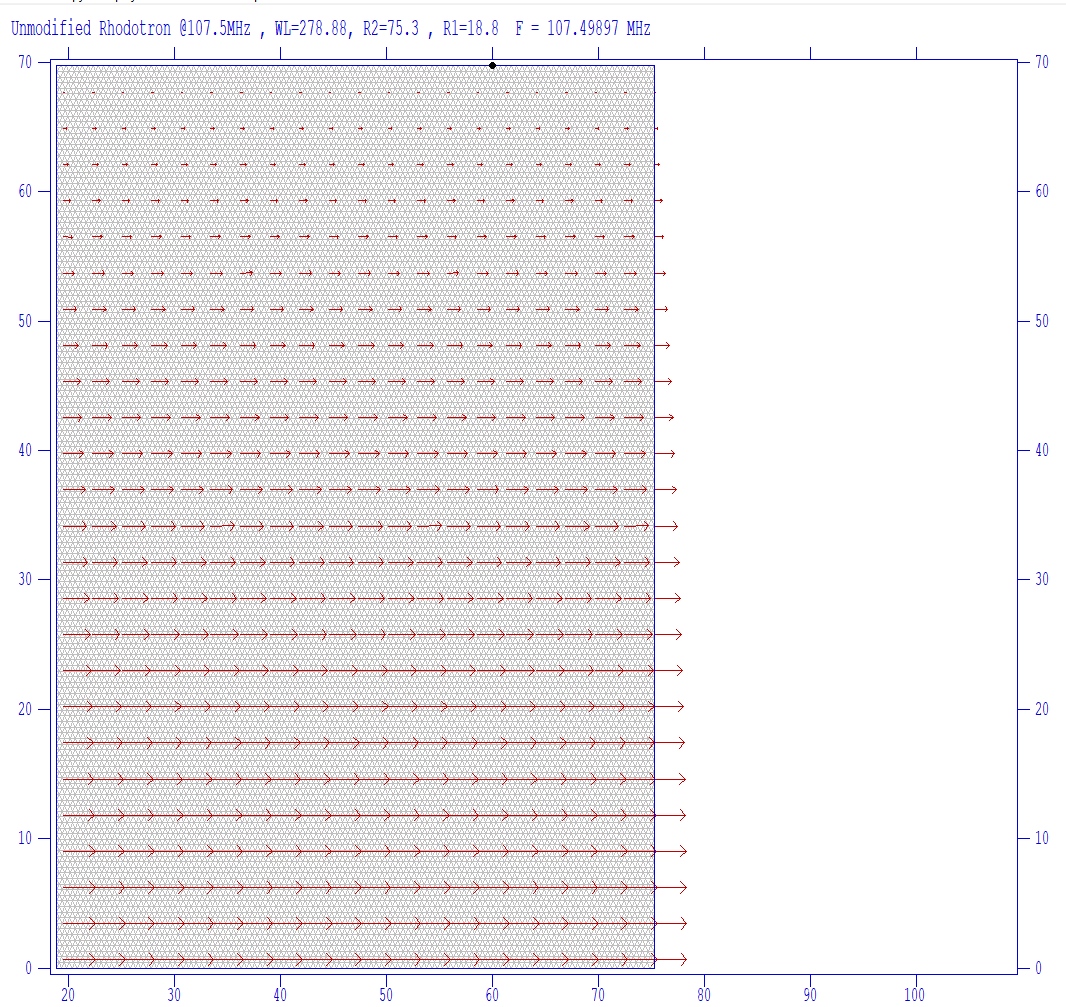
\includegraphics[width=\linewidth]{./figures/superfish/superfish107.png}
      \caption{107.5 MHz}
    \end{subfigure}%
    \centering
    \begin{subfigure}{.5\textwidth}
      \centering
      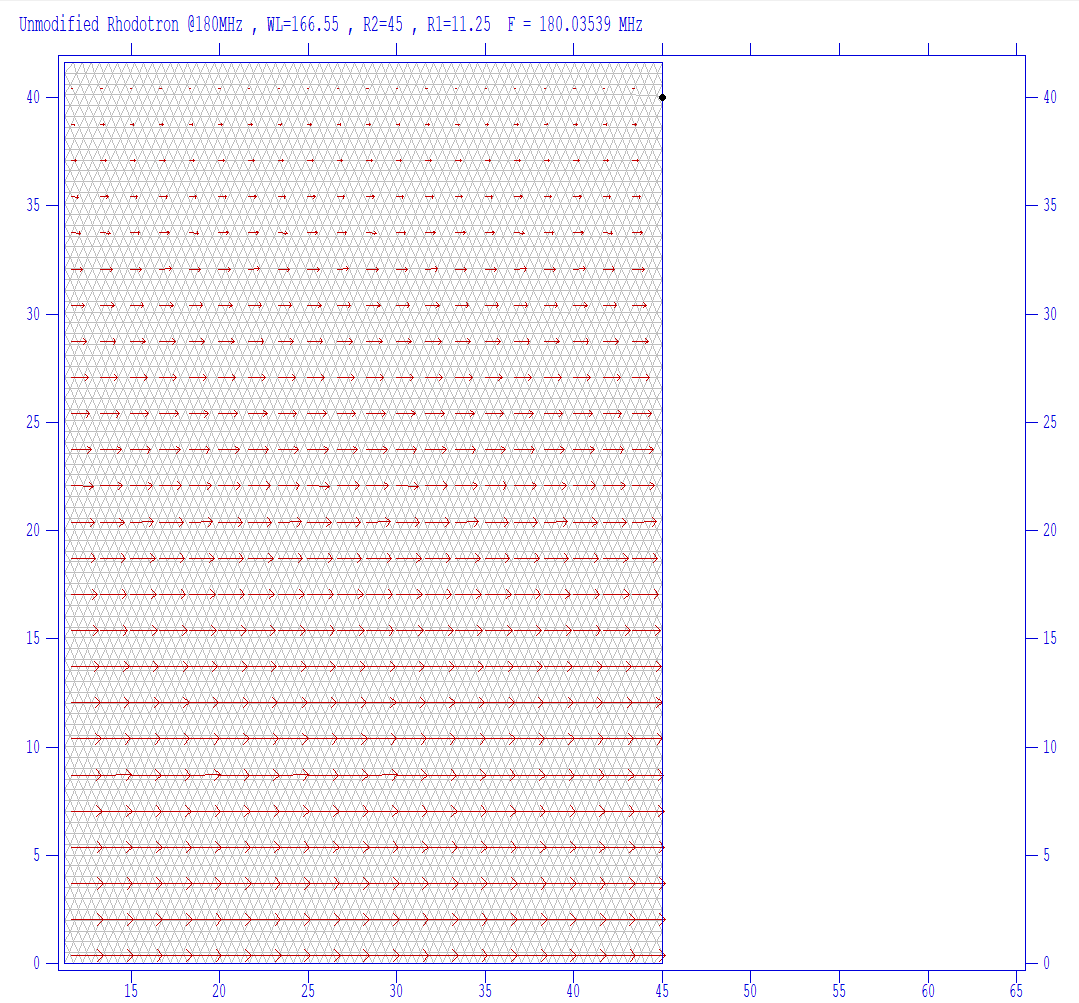
\includegraphics[width=\linewidth]{./figures/superfish/superfish180.png}
      \caption{180 MHz}
    \end{subfigure}
    \caption{Poission Superfish results for \fromeq{107_180_MHZ_cavity_design_parameters}}
    \label{fig:107_simple_cavity_design}
\end{figure}

\begin{figure}[H]
    \centering
    \begin{subfigure}{.5\textwidth}
      \centering
      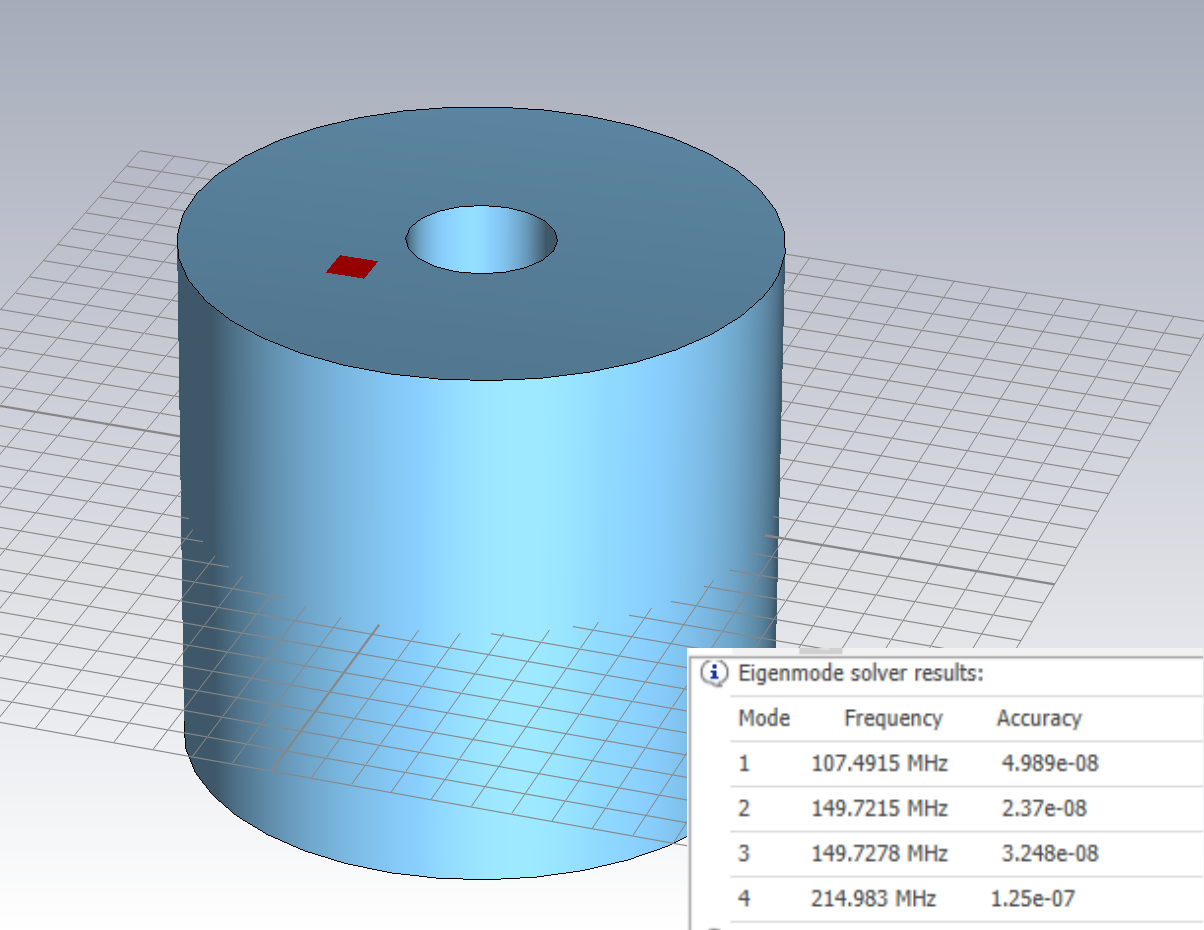
\includegraphics[width=\linewidth]{./figures/cst/cst107.png}
      \caption{107.5 MHz}
    \end{subfigure}%
    \begin{subfigure}{.5\textwidth}
      \centering
      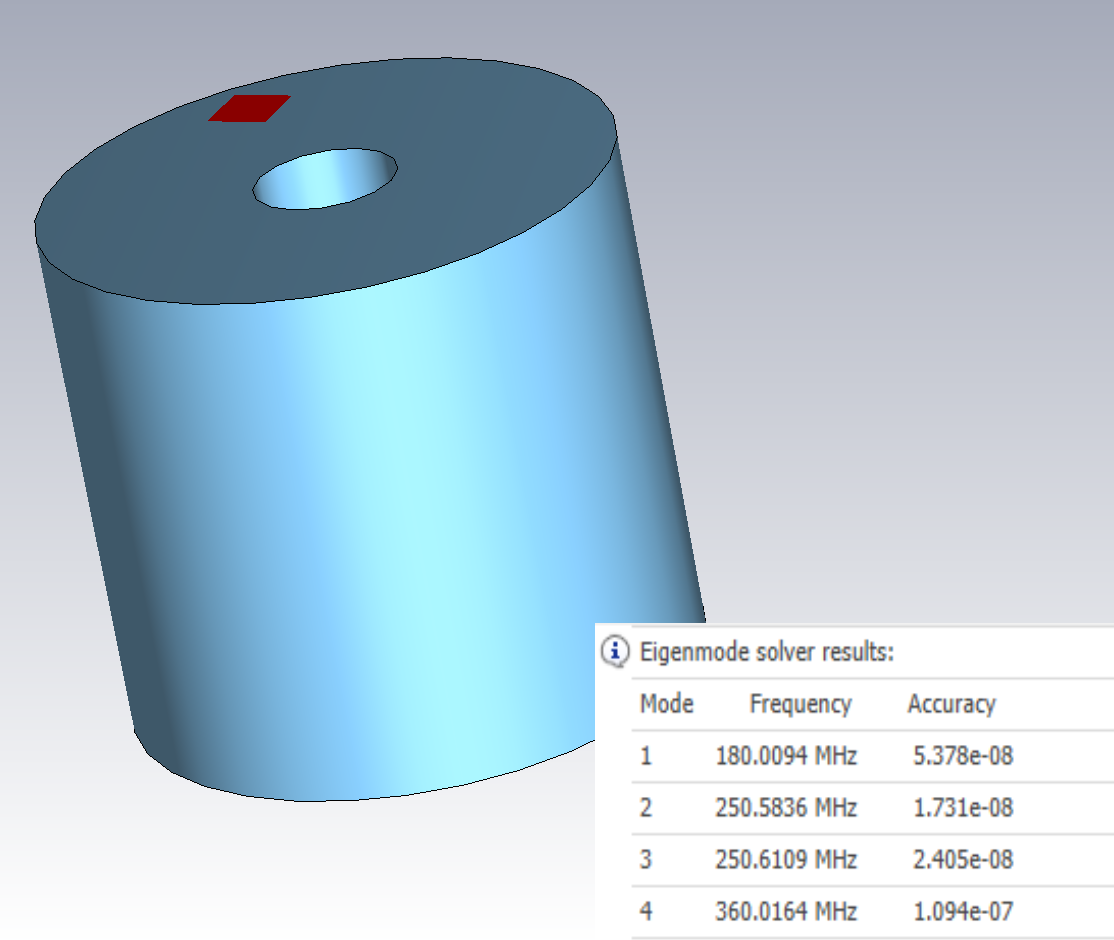
\includegraphics[width=.9\linewidth]{./figures/cst/cst180.png}
      \caption{180 MHz}
    \end{subfigure}
    \caption{CST Eigenmode results for \fromeq{107_180_MHZ_cavity_design_parameters}}
    \label{fig:180_simple_cavity_design}
\end{figure}

\begin{figure}[H]
    \centering
    \begin{subfigure}{.5\textwidth}
      \centering
      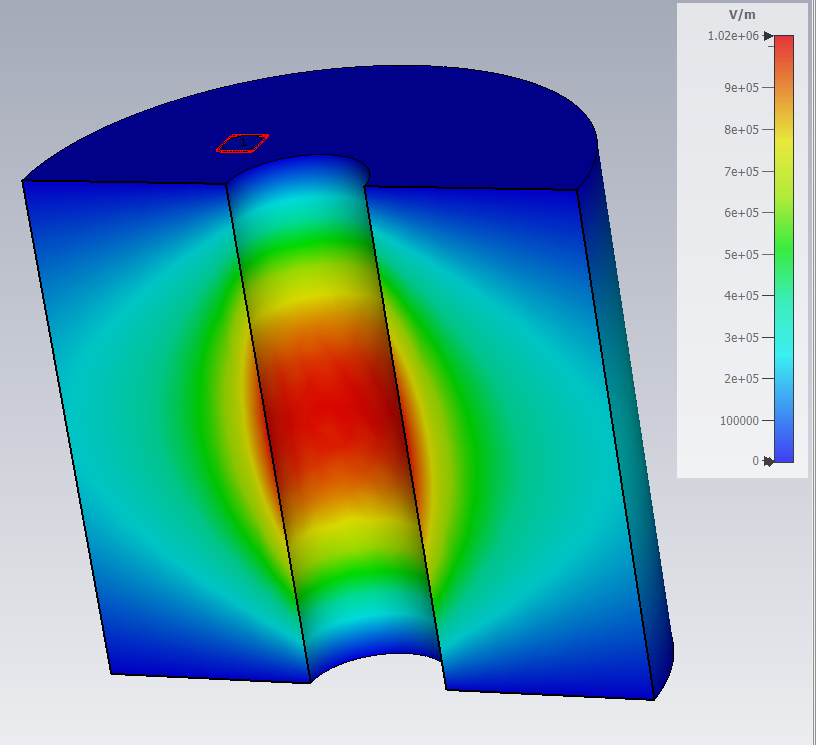
\includegraphics[width=.9\linewidth]{./figures/cst/cst107_e.png}
      \caption{107.5 MHz}
    \end{subfigure}%
    \begin{subfigure}{.5\textwidth}
      \centering
      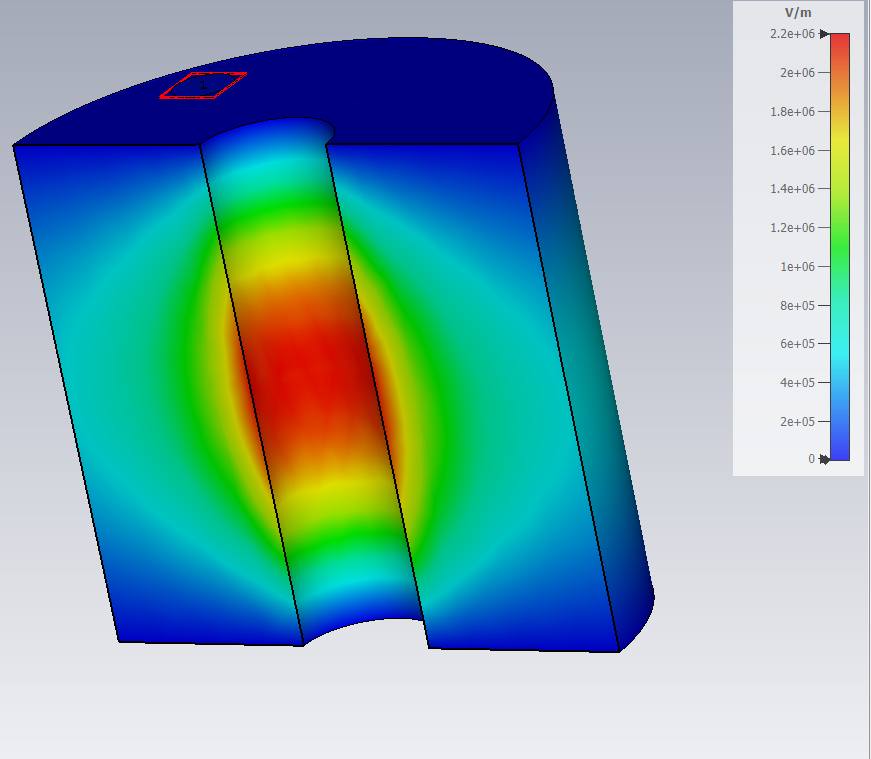
\includegraphics[width=.94\linewidth]{./figures/cst/cst180_e.png}
      \caption{180 MHz}
    \end{subfigure}
    \caption{CST Electric field solutions for \fromeq{107_180_MHZ_cavity_design_parameters}}
    \label{fig:cst_simple_cavity_designs}
\end{figure}
As mentioned by POTTIER, truncated cone terminations in inner cylinder can improve the shunt empedance $Z$ of the cavity \cite{rhodo_pottier}. 
Below, \textit{Poission superfish} results of such a modification with matching height increase to keep resonant frequency can be found.
\begin{figure}[H]
    \centering
    \begin{subfigure}{.5\textwidth}
      \centering
      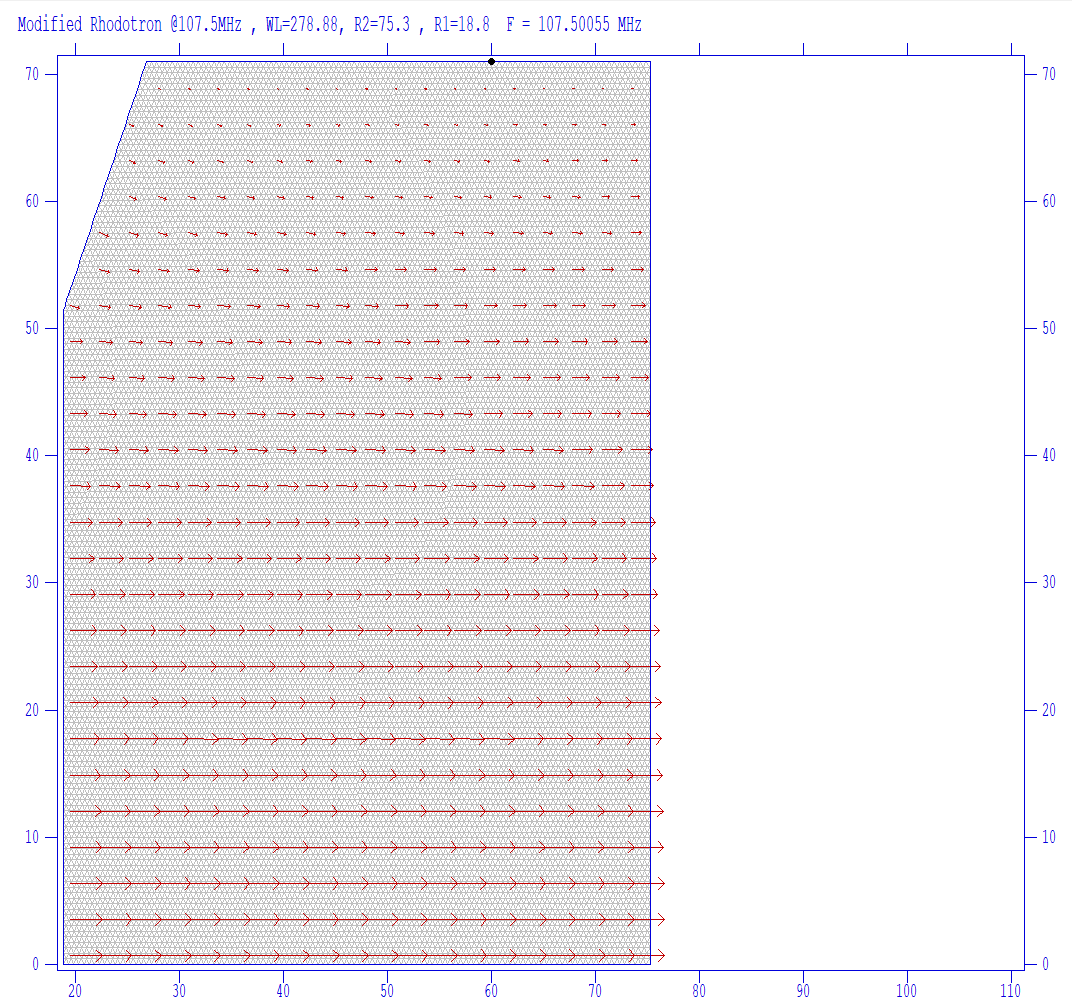
\includegraphics[width=.9\linewidth]{./figures/superfish/superfish107mod.png}
      \caption{107.5 MHz truncated}
    \end{subfigure}%
    \begin{subfigure}{.5\textwidth}
      \centering
      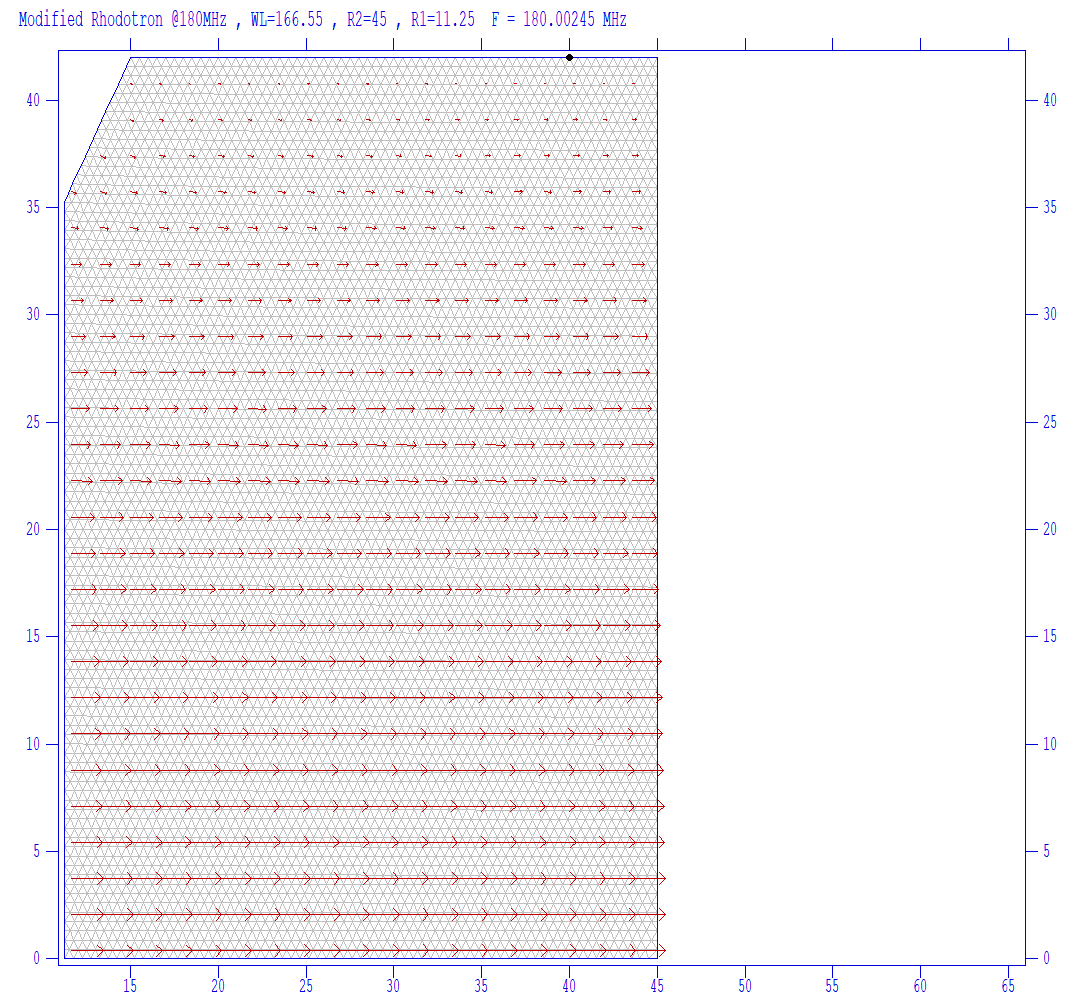
\includegraphics[width=.9\linewidth]{./figures/superfish/superfish180mod.png}
      \caption{180 MHz truncated}
    \end{subfigure}
    \caption{Poisson SUPERFISH field results of truncated cavities}
    \label{fig:107_180_modified_cavities_superfish}
\end{figure}

\begin{figure}[H]
    \centering
    \begin{subfigure}{.5\textwidth}
      \centering
      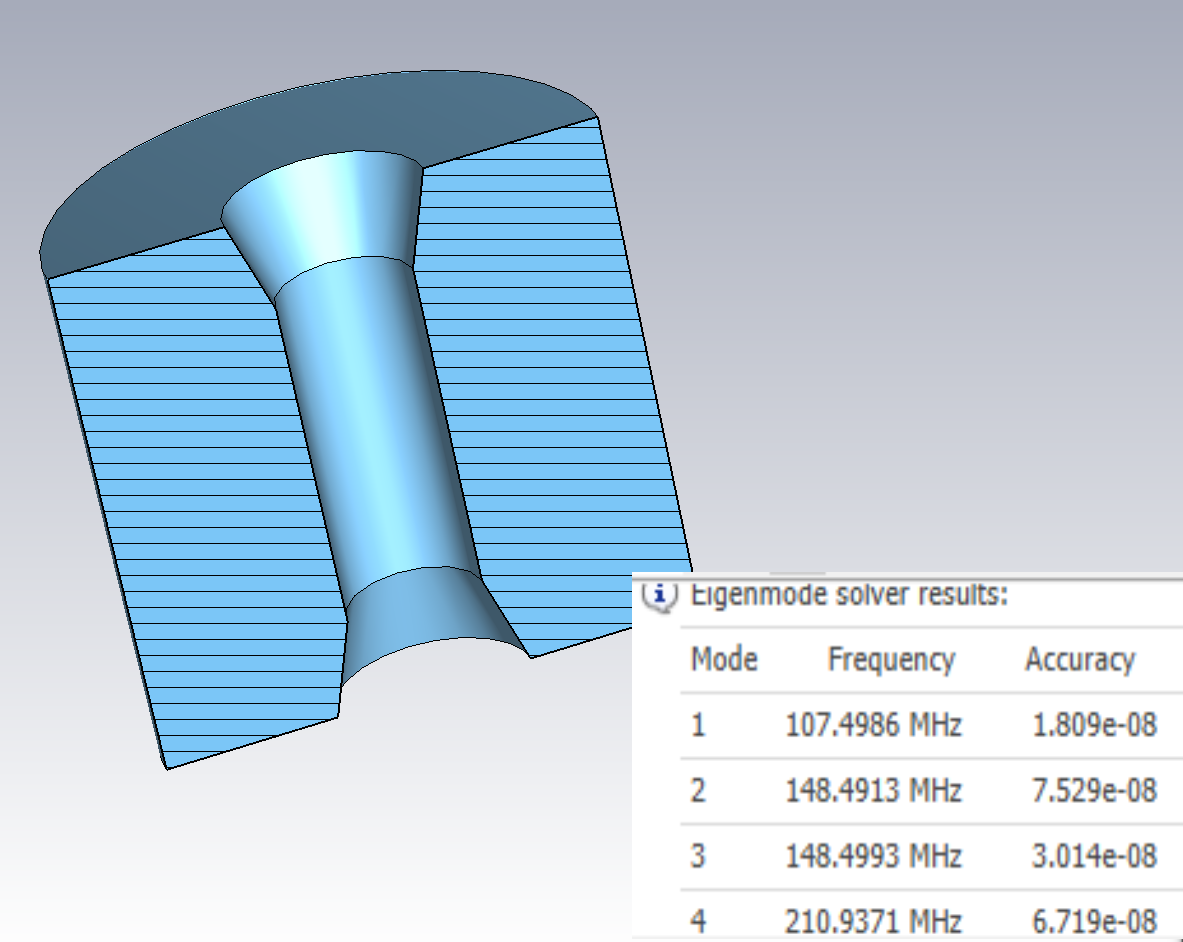
\includegraphics[width=.9\linewidth]{./figures/cst/cst107mod.png}
      \caption{107.5 MHz truncated}
    \end{subfigure}%
    \begin{subfigure}{.5\textwidth}
      \centering
      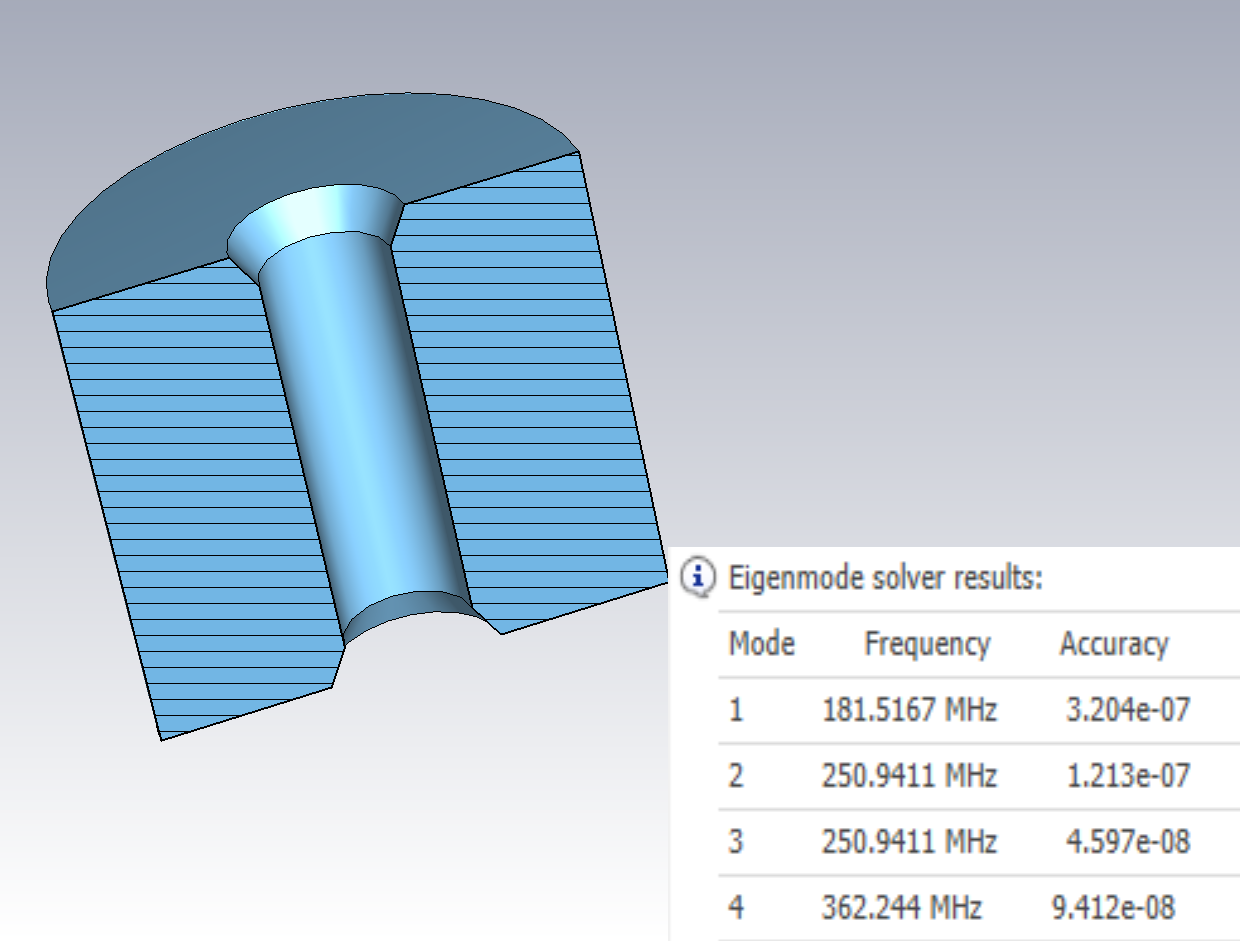
\includegraphics[width=.9\linewidth]{./figures/cst/cst180mod.png}
      \caption{180 MHz truncated}
    \end{subfigure}
    \caption{CST eigenmode results of truncated cavities}
    \label{fig:107_180_modified_cavities_cst_eigenmode}
\end{figure}

\begin{figure}[H]
    \centering
    \begin{subfigure}{.5\textwidth}
      \centering
      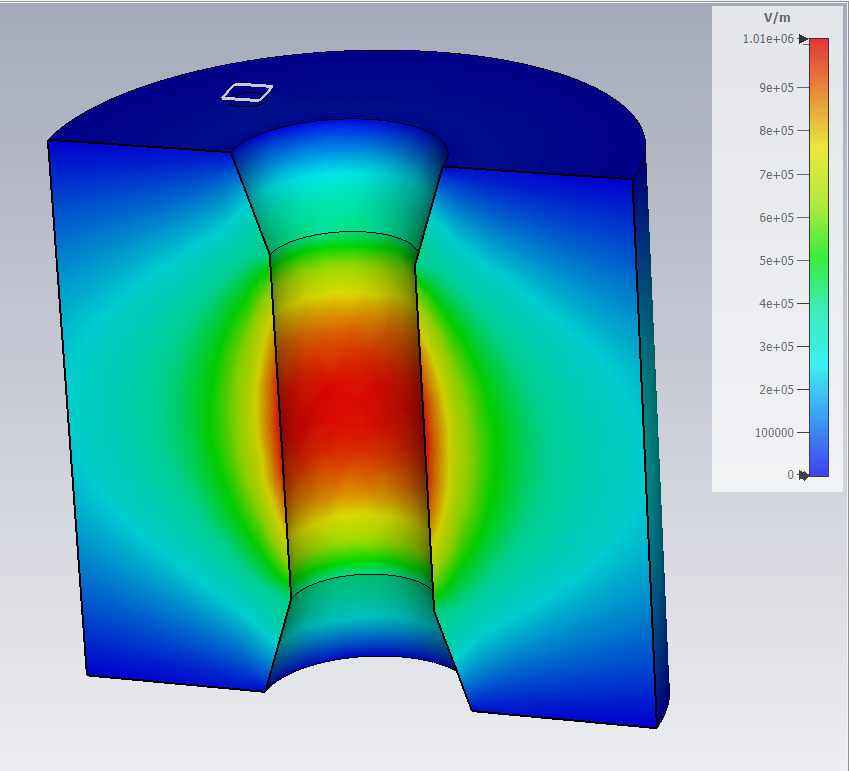
\includegraphics[width=.9\linewidth]{./figures/cst/cst107mod_e.png}
      \caption{107.5 MHz truncated}
    \end{subfigure}%
    \begin{subfigure}{.5\textwidth}
      \centering
      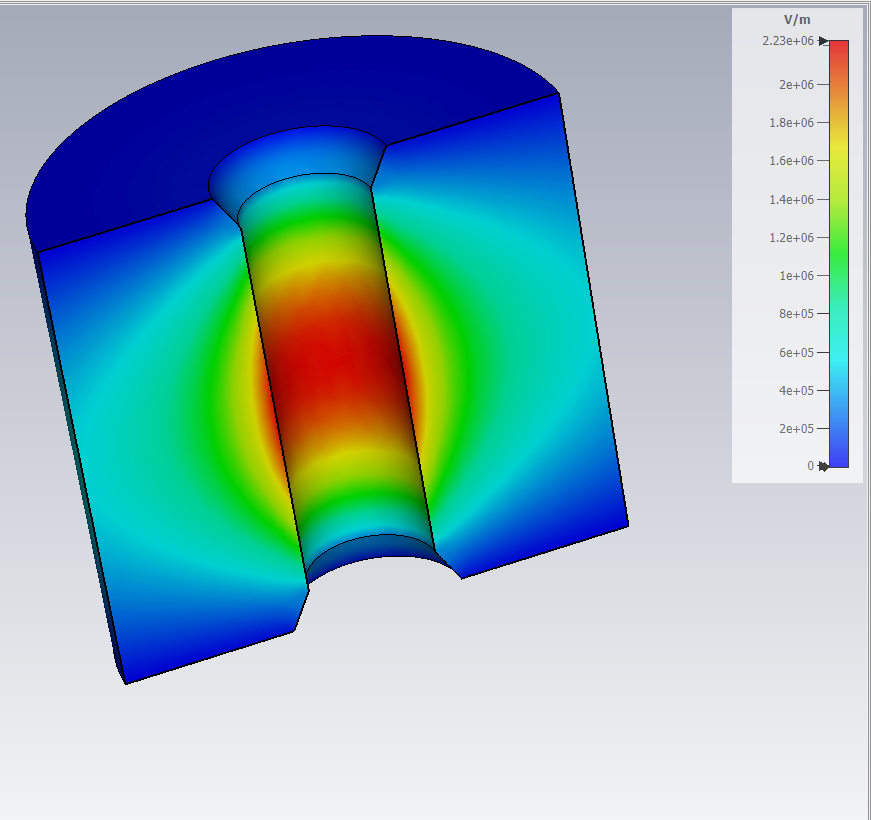
\includegraphics[width=.88\linewidth]{./figures/cst/cst180mod_e.png}
      \caption{180 MHz truncated}
    \end{subfigure}
    \caption{CST electric field results of truncated cavities}
    \label{fig:107_180_modified_cavities_cst_field}
\end{figure}

\begin{figure}[H]
    \centering
    \begin{subfigure}{.5\textwidth}
      \centering
      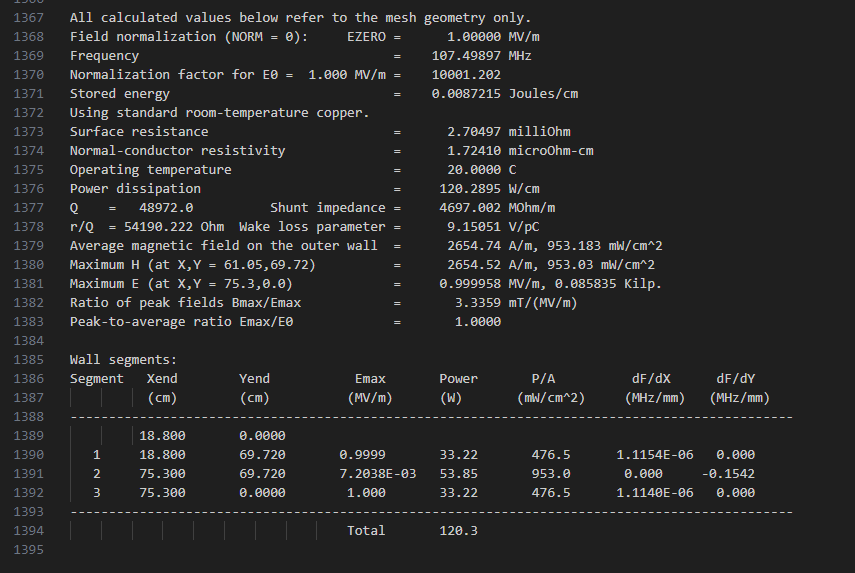
\includegraphics[width=0.97\linewidth]{./figures/superfish/superfish107_z.png}
      \caption{107.5 MHz unmodified}
    \end{subfigure}%
    \begin{subfigure}{.5\textwidth}
      \centering
      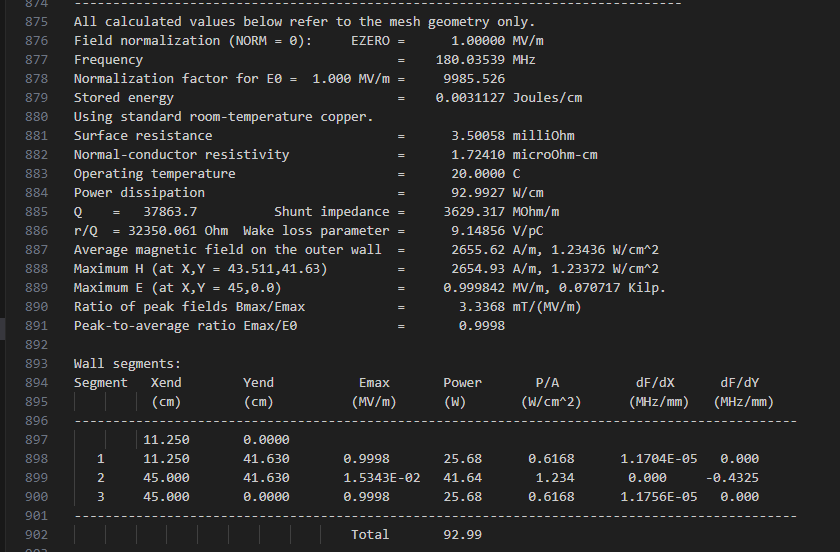
\includegraphics[width=0.99\linewidth]{./figures/superfish/superfish180_z}
      \caption{180 MHz unmodified}
    \end{subfigure}
    \caption{Poisson Superfish calculations with \textit{unmodified} cavities}
    \label{fig:107_cavity_shunt_diff}
\end{figure}
    
\begin{figure}[H]
    \centering
    \begin{subfigure}{.5\textwidth}
      \centering
      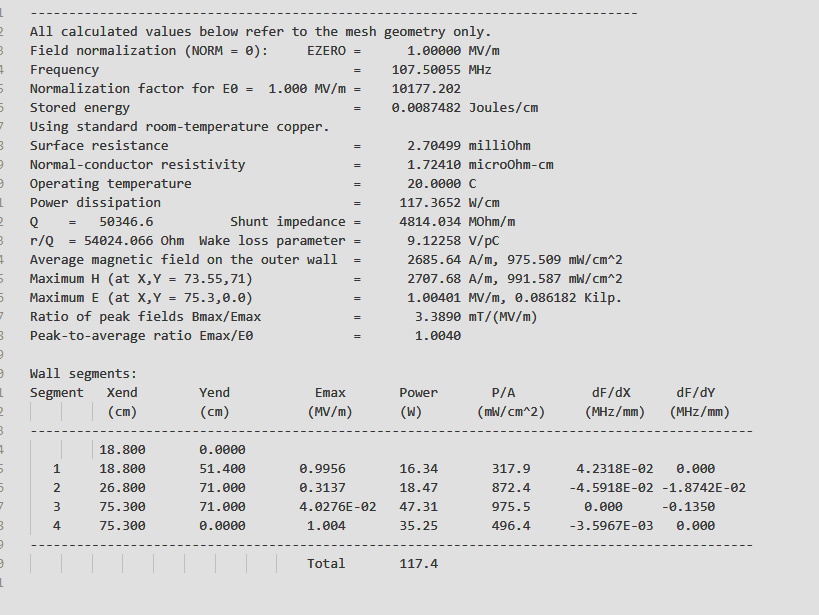
\includegraphics[width=0.95\linewidth]{./figures/superfish/superfish107mod_z.png}
      \caption{107.5 MHz truncated}
    \end{subfigure}%
    \begin{subfigure}{.5\textwidth}
      \centering
      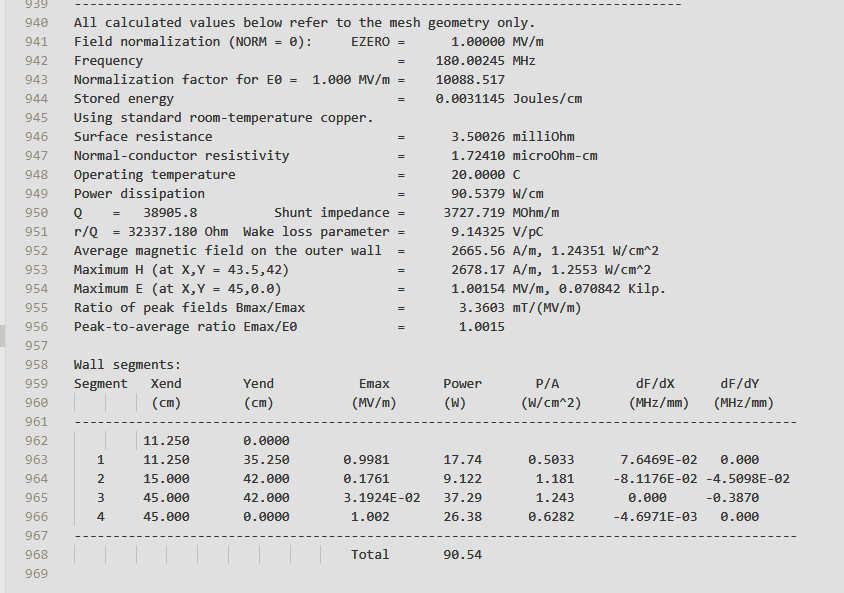
\includegraphics[width=\linewidth]{./figures/superfish/superfish180mod_z.png}
      \caption{180 MHz truncated}
    \end{subfigure}
    \caption{Poisson Superfish calculations with \textit{truncated} cavities}
    \label{fig:180_cavity_shunt_diff}
\end{figure}
One can observe the shunt impedance gain between truncated and unmodified cavities in \fromfigs{107_cavity_shunt_diff}{180_cavity_shunt_diff};
\begin{equation*}
    \begin{aligned}
        \Delta Z_{107.5}=2.5\%
    \end{aligned}
    \qquad
    \begin{aligned}
        \Delta Z_{180}=2.7\%
    \end{aligned}
\end{equation*}



\section{Magnet Design} \label{sec:magnet_design}
Magnet design in rhodotron type accelerators depend heavily on the design of the cavities.
Because the limiting factors usually are frequency and total volume of the accelerator, magnet design parameters are considered after cavity design has been completed.
Considering the nature of coaxial cavity, simplest path for beams inside magnets is major segment of a circle, which was used as the reference for following discussions.
\begin{figure}[H]
    \captionsetup[subfigure]{justification=centering}
    \captionsetup{justification=centering}
    \centering
    \begin{subfigure}{.5\textwidth}
      \centering
      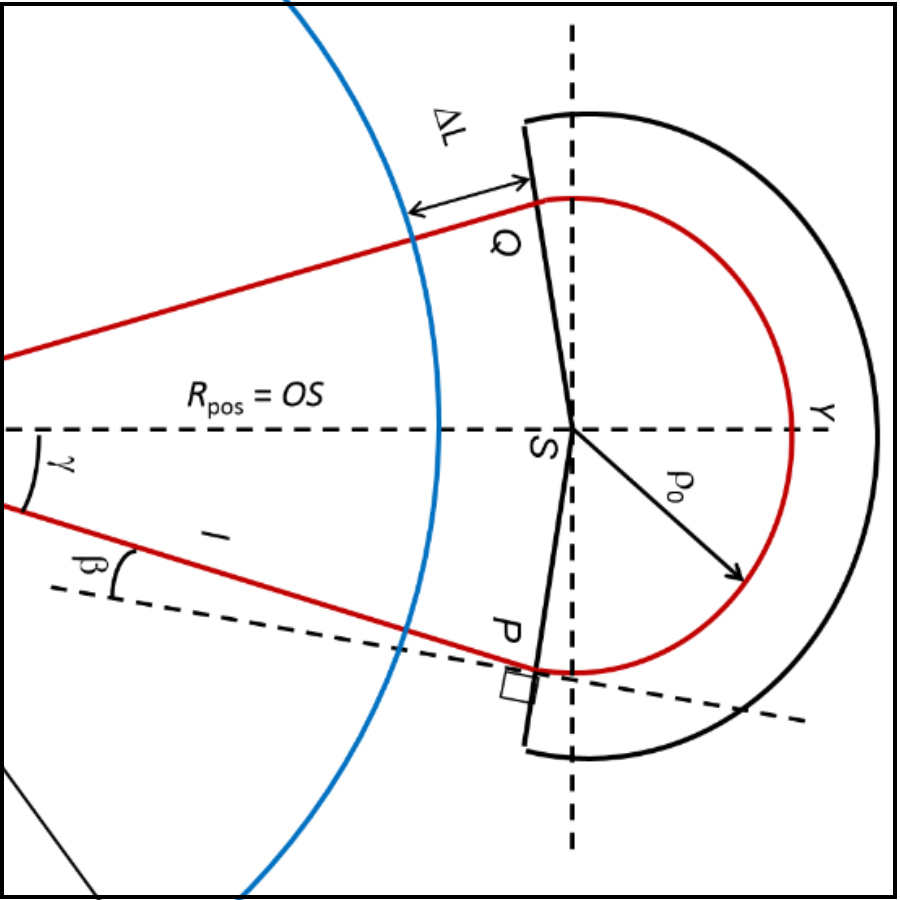
\includegraphics[width=.9\linewidth]{./figures/design/Ltot.png}
    \end{subfigure}%
    \centering
    \begin{subfigure}{.5\textwidth}
      \centering
      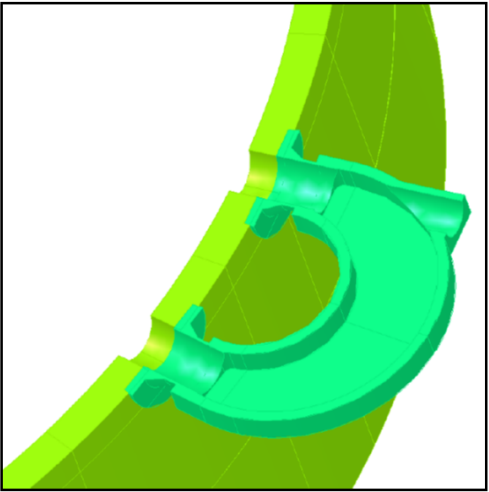
\includegraphics[width=.9\linewidth]{./figures/design/tt300_mag.png}
    \end{subfigure}
    \caption{Geometry and modeling, outside trajectory of a rhodotron (TT300) \cite{cite:rhodo_design}}
    \label{fig:magnet_design_illustrations}
\end{figure}
In rhodotron accelerators, magnets are used for not only guiding the electron beam to desired path, but also for syncronizing them with the RF field in the cavity. 
This syncronization, also called phase stability, is the fundamental constraint of magnet design. 
Time spent outside of the RF cavity should be precisely tuned to maximize acceleration in the succeeding pass. 

Two different approaches have been used to achieve phase stability.
These approaches are discussed further in the following sections.

\subsection{$n\lambda$ Technique} \label{sec:n_L_technique}

First approach for phase stability considiration assumes that from the start of the current pass, $\beta_{avg} \approx 1$ for a synchronous particle. 

To maintain the phase synchronization, a particle that started the current pass at $t=0$, should start the next pass at $t=nT$, where $n$ is an integer and $T$ is the period of RF field inside cavity.
As discussed earlier, by assuming the electron is traveling at $c$, phase stability can be achieved by designing the whole trajectory to be $n \lambda$, where $\lambda$ is the wavelength of the RF field. 
In other words, total trajectory of synchronous particle needs to satisfy the following equality:
\begin{equation}
    L_{pass} = n \lambda
\end{equation} 
Since $n>1$ would require unnecessarily long and expensive beam guide and magnets, $n=1$ is the most efficient choice:
\begin{equation}
    L_{pass} = \lambda
\end{equation} 

\begin{figure}[H]    
    \centering
    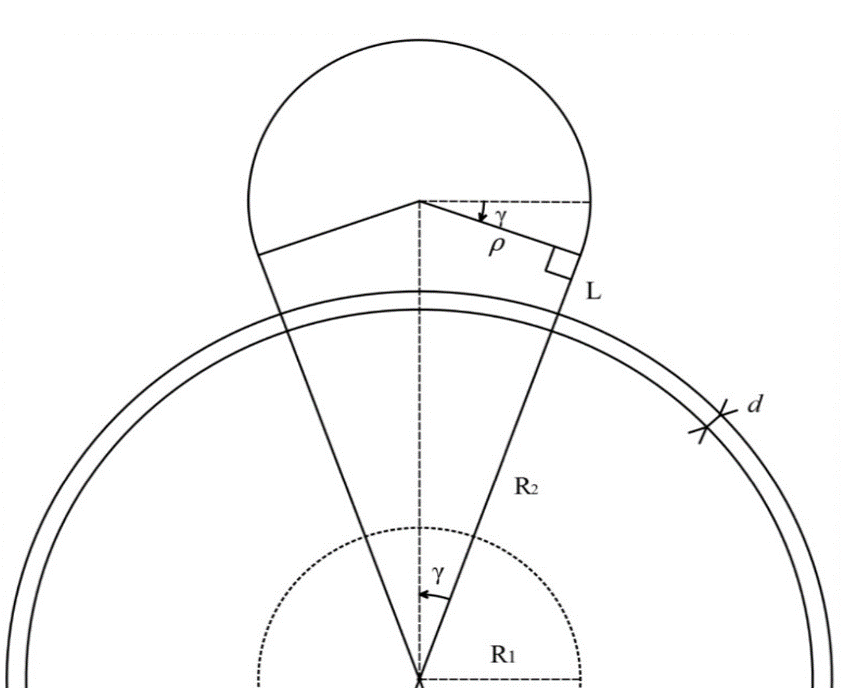
\includegraphics[width=.8\linewidth]{./figures/design/magnet_design.png}
    \caption{Trejectory of a particle in single pass}
    \label{fig:magnet_design}
\end{figure}
From \fromfig{magnet_design}, where $\gamma$ is half the angle between trajectories of successive passes, $\rho$ is the radius of the circular path inside magnet, 
$L$ is the length of the magnet guide, $d$ is the thickness of the RF cavity wall:
\begin{eqnarray}
    L_{in} &=& 2R_2 \nonumber\\
    L_{out} &=& 2L + 2d + (\pi + 2\gamma)\rho \nonumber \\
    L_{pass} &=& L_{in} + L_{out}  \nonumber \\
    \lambda &=& 2R_2 + 2d + 2L + (\pi + 2\gamma)\rho \label{eq:magnet_lambda_constraint}
\end{eqnarray}
After the cavity design is complete, only $L$, $\gamma$ and $\rho$ remain, which are the design parameters of magnets.
Observing the \fromfig{magnet_design} and using \fromeq{magnet_lambda_constraint},
\begin{eqnarray}
    \tan (\gamma) &=& \frac{\rho}{R_2 + d + L} \nonumber \\
    \rho &=&  \tan (\gamma) (R_2 + d + L) \nonumber\\
    2\rho &=& \tan (\gamma) (\lambda - (\pi + 2\gamma)\rho) \nonumber\\
    \rho (2 + \tan (\gamma)(\pi + 2\gamma)) &=&  \tan (\gamma) \lambda \nonumber\\
    \rho &=& \frac{\lambda}{\pi + 2\gamma + \frac{2}{\tan (\gamma)}} \label{eq:magnet_rho_constraint} \\
    L + d &=& \frac{\rho}{\tan (\gamma)} - R_2 \label{eq:magnet_L_constraint}
\end{eqnarray}
\textit{Equations \ref{eq:magnet_rho_constraint} and \ref{eq:magnet_L_constraint}} define 2 constraints. As already discussed, it has been assumed that cavity design is set (\textit{i.e} $R_2$, $\lambda$, $d$ are already defined).
Therefore only the magnet design parameters $\rho$, $\gamma$ and $L$ are left. Together with the constraints, one free variable defines the whole magnet design. 
Considering the importance of $\gamma$ for maximum number of possible passes, it will be used as the free magnet design variable in the further discussions.


\subsection{$L_{out}$ Parameter Sweep} \label{sec:parameter_sweep}

As mentioned previously in \fromsec{n_L_technique}, \fromeq{magnet_lambda_constraint} assumes that the particles are fast enough so that $\Delta t_{pass} \approx n T$. 
This assumption is not guaranteed however, especially in the first few passes if the particles are not accelerated enough. 
This scenario can happen when RF power is not sufficiently high. 

Consider an RF supply with $f=1$ GHz, $P=50$ kW. Using \fromeq{W_total_gain_pottier}, 
after the first pass the synchronous electron that entered the accelerator with $40$ keV and $\phi=15^\circ$ phase lag,
\begin{eqnarray*}
    W_{gain} &=& 2.14\times0.2998^{1/4}\times 50000^{1/2} = 354keV \\
    W_{total} &=& 394 keV \\
    \beta_{40keV} &\approx& 0.374 \\
    \beta_{394keV} &\approx& 0.825
\end{eqnarray*}
It is clear that $\beta_{avg}$ is not fast enough to sustain phase stability if the magnet is designed for $\beta = 1$. 
For these cases, \fromeq{magnet_lambda_constraint} fails to deliver phase stability.
Another approach for designing a magnet would be to find a new constraint, $K$ for total path length.
\begin{eqnarray*}
    L_{pass} &=& K \\
    L_{in} + L_{out} &=& K
\end{eqnarray*}
Since $L_{in}$ is set previously from cavity design, we can remove it from our equation and continue with
\begin{equation} \label{eq:mag_sweep_constraint}
    L_{out} = K
\end{equation}
To start, an optimization criteria for the following pass such as
\begin{itemize}
    \item Ensure the phase stability of the synchronous electron
    \item Maximize the energy gain of the synchronous electron
    \item Minimize the energy spread of the beam
    \item Minimize the phase lag spread of the beam
    \item All of the above with decided weights
\end{itemize}
needs be selected. Using a simulation software such as \textit{CST Studio Particle Module}, the optimum value of $K$ for the criteria can be found by simulating for different values of $K$ (\textit{sweeping}) and analyzing the results.
This process can be repeated for each magnet until the desired beam characteristics in the end of the accelerator are achieved.

However, one caviat of this technique is that, available simulation softwares are not well suited for this kind of process. As mentioned above, \textit{CST Studio Particle Module} has a \textit{parameter sweep} functionality.
But the calculation times are too slow to be useful in this particular problem. \textit{A custom built software offering magnet optimizing sweep functionality will be discussed in the following chapter.}




\section{Initial Design at KAHVELab} 

A rhodotron with operation frequency of $107.5$ MHz was decided to be built at KAHVELab. 
Frequency was selected to benefit from the RF power supply units at hand.
After considering the earlier simulations mentioned in \fromsecs{cavity_design}{magnet_design}, an initial design was created.
\begin{figure}[H]
    \centering
    \captionsetup{justification=centering}
    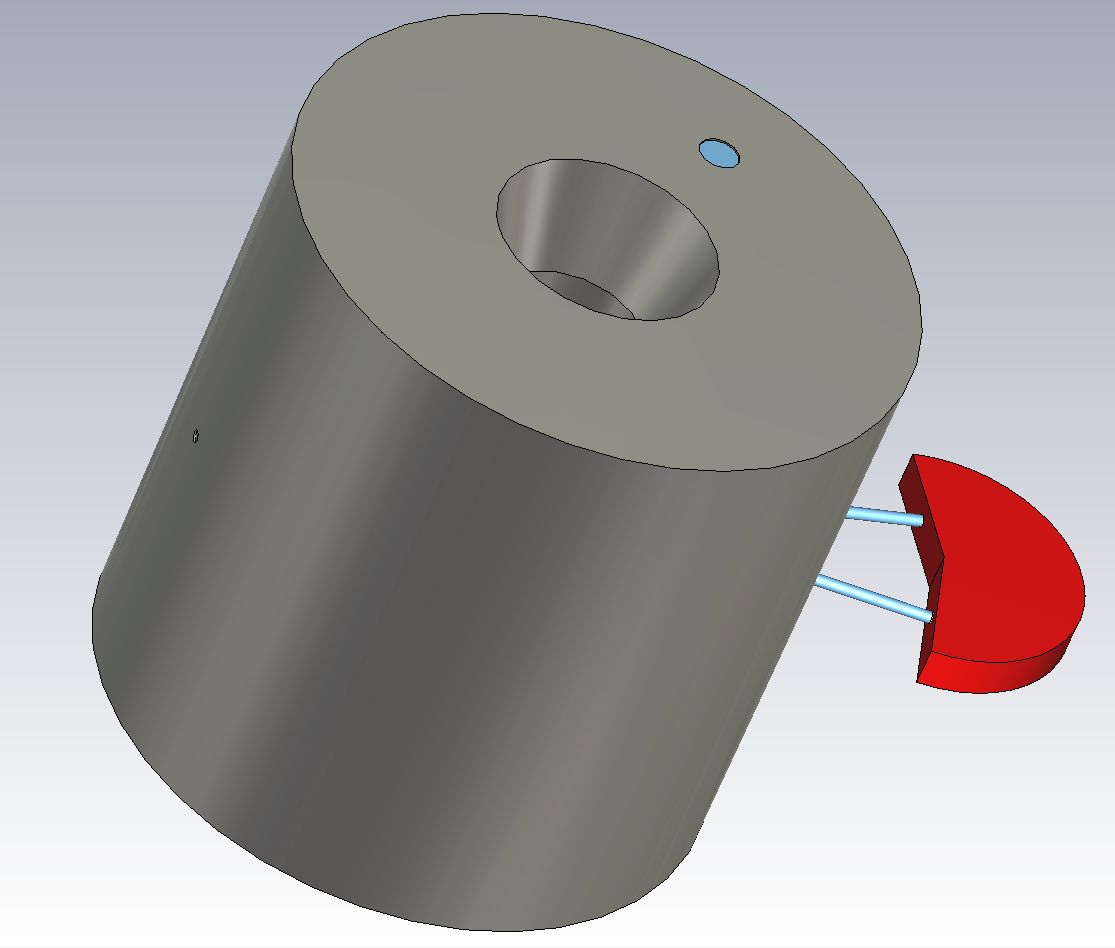
\includegraphics[width=.5\linewidth]{./figures/cst/cst_first_design1.png}
    \caption{Initial design of the proposed rhodotron \\ $\gamma=9^\circ$}
    \label{fig:initial_design}
\end{figure}
\begin{figure}[H]
    \captionsetup[subfigure]{justification=centering}
    \captionsetup{justification=centering}
    \centering
    \begin{subfigure}{.5\textwidth}
      \centering
      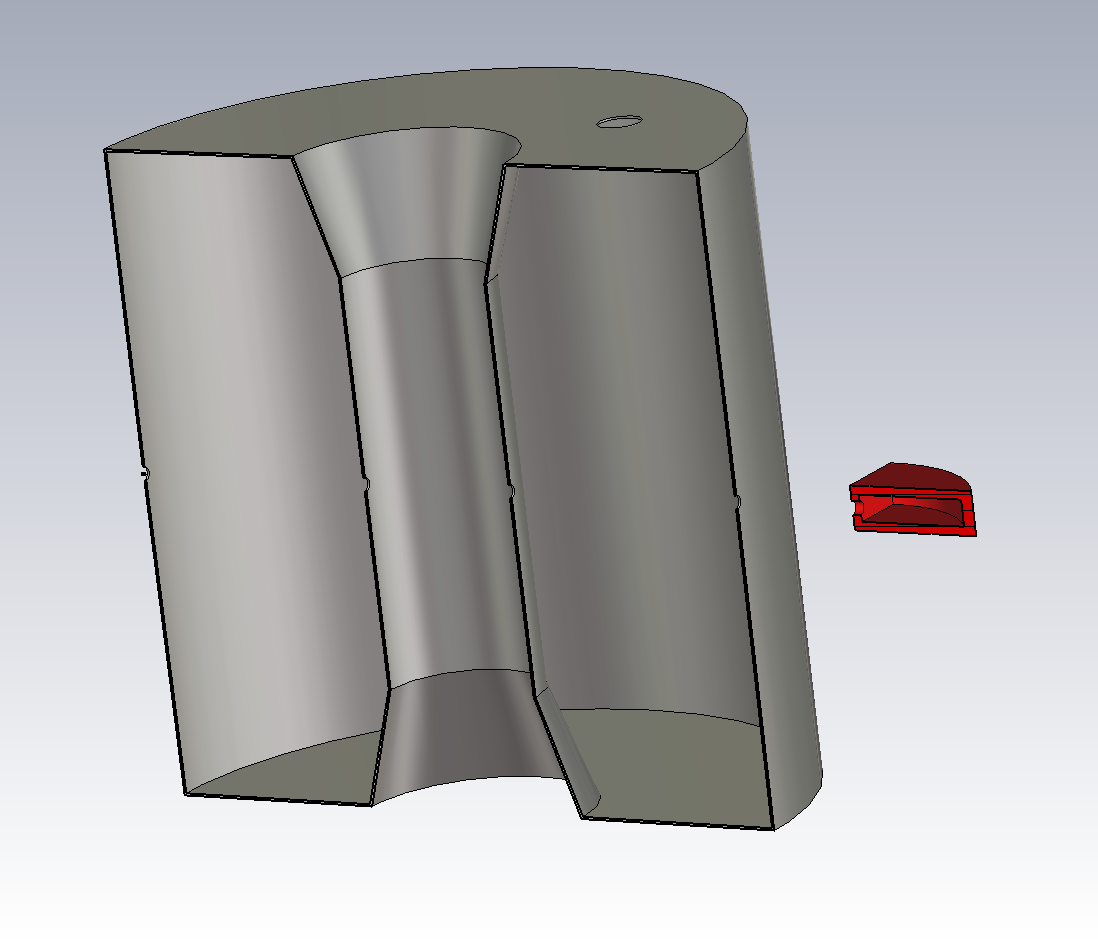
\includegraphics[width=.92\linewidth]{./figures/cst/cst_first_design3.png}
      \caption{Axial cross section.}
    \end{subfigure}%
    \centering
    \begin{subfigure}{.5\textwidth}
      \centering
      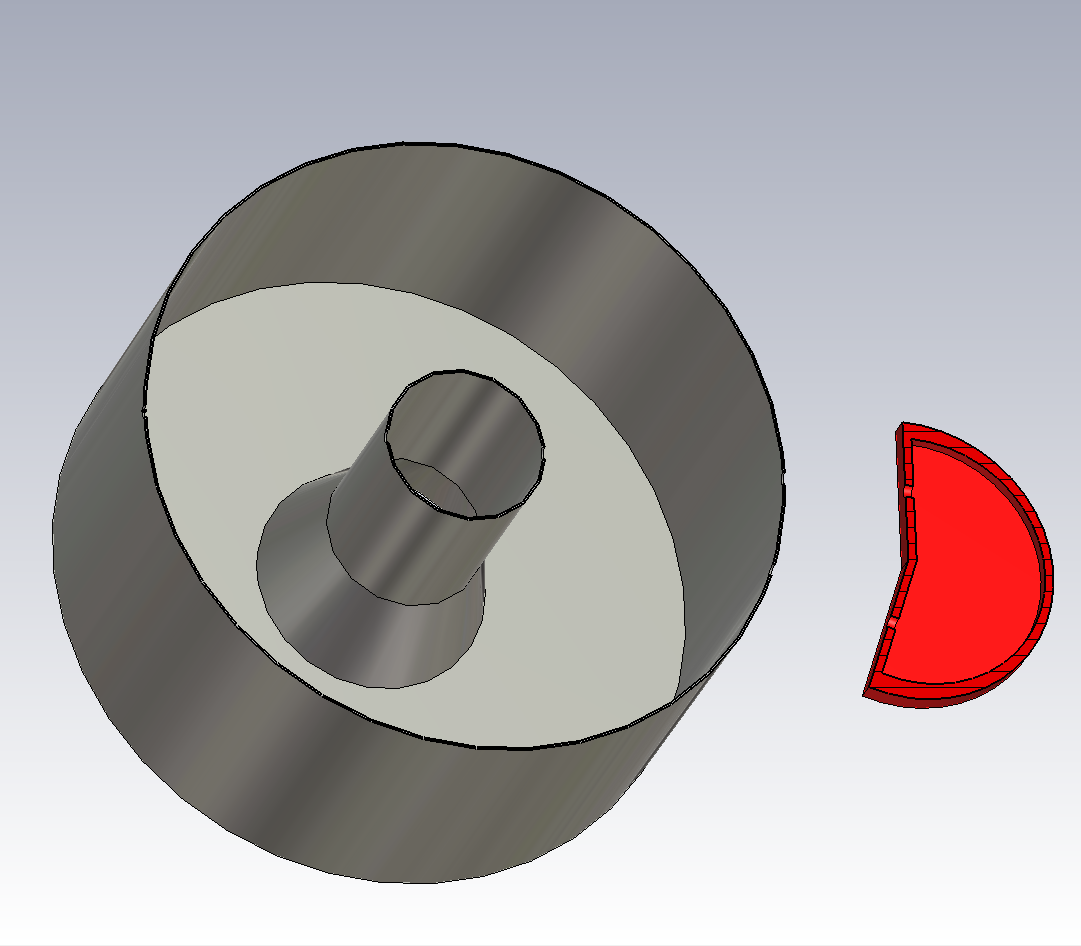
\includegraphics[width=.9\linewidth]{./figures/cst/cst_first_design2.png}
      \caption{Cross section at acceleration plane.}
    \end{subfigure}
    \caption{Initial design of the proposed rhodotron.}
    \label{fig:initial_design_cross_section}
\end{figure}
The magnets used in this design is the simplest in terms of design parameters. It consists of an iron casing encapsulating the shape of desired magnetic field, which are created by two coils inside.
\begin{figure}[H]
    \captionsetup[subfigure]{justification=centering}
    \captionsetup{justification=centering}
    \centering
    \begin{subfigure}{.5\textwidth}
      \centering
      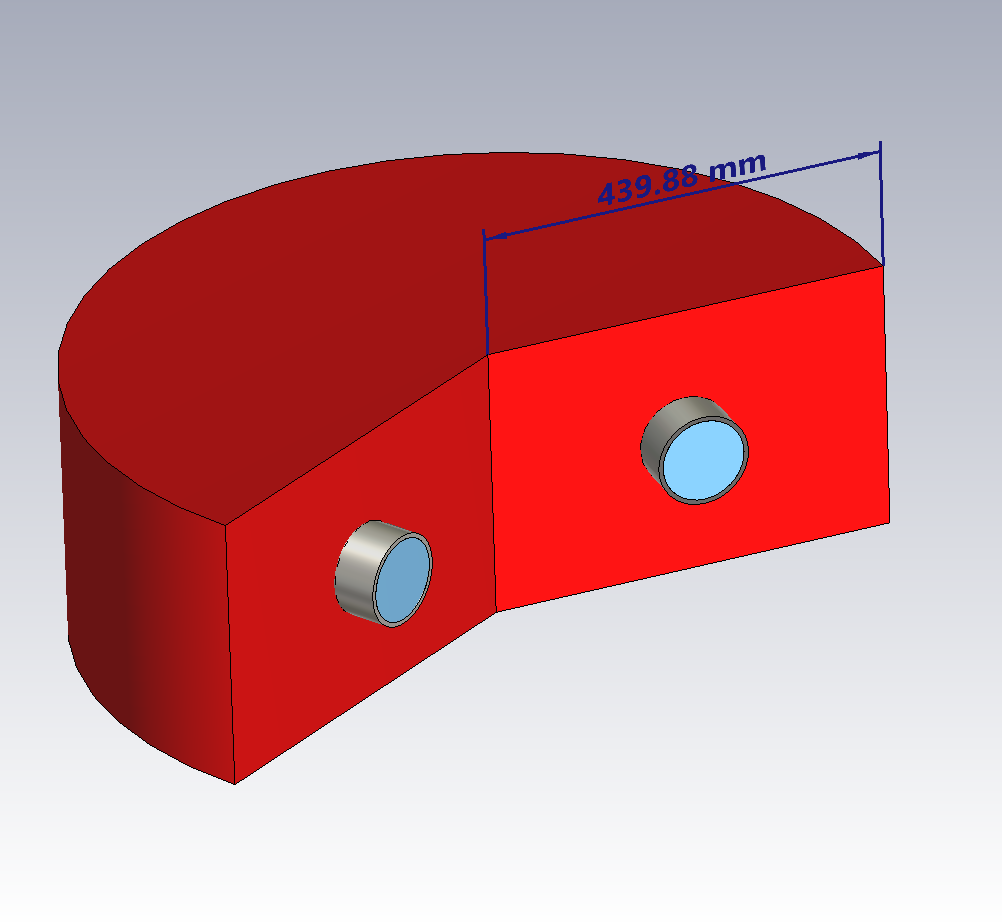
\includegraphics[width=.9\linewidth]{./figures/cst/cst_first_magnet_design1.png}
    \end{subfigure}%
    \centering
    \begin{subfigure}{.5\textwidth}
      \centering
      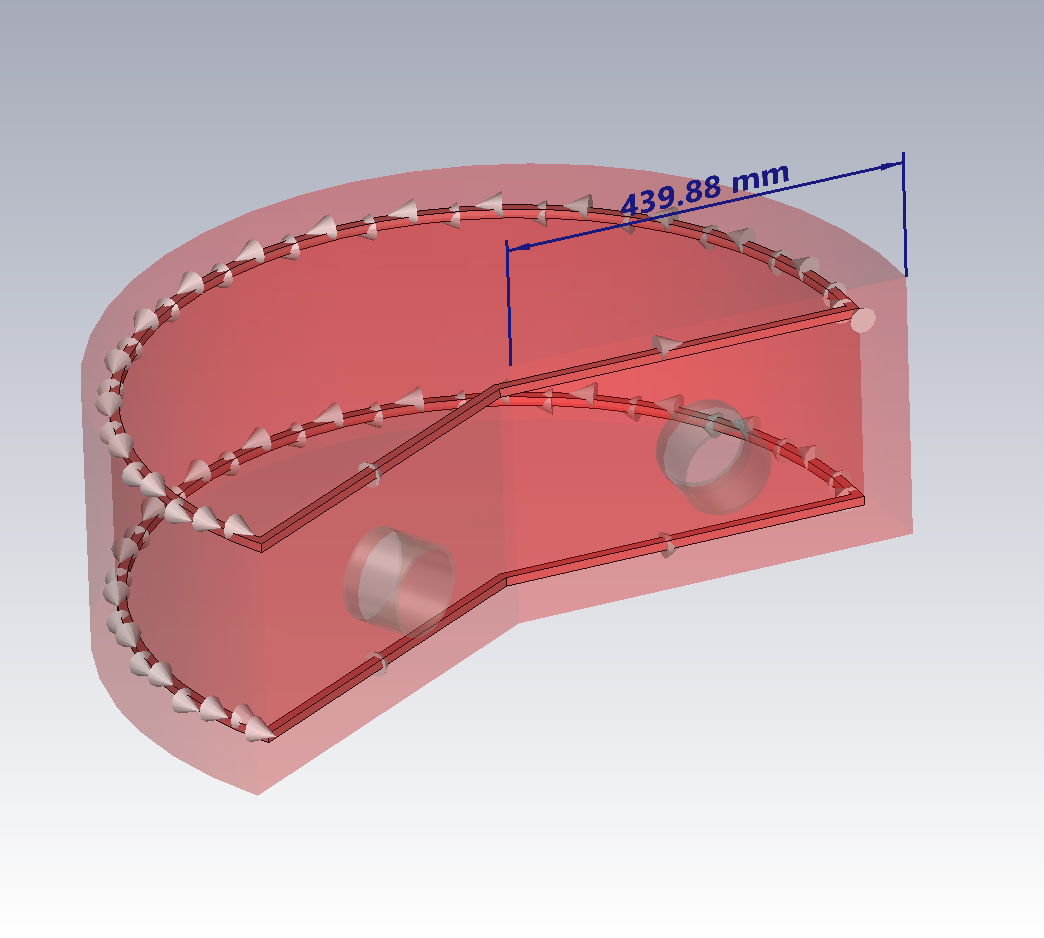
\includegraphics[width=.92\linewidth]{./figures/cst/cst_first_magnet_design2.png}
    \end{subfigure}
    \caption{Initial magnet design.}
    \label{fig:initial_magnet_design}
\end{figure}

\begin{figure}[H]
    \centering
    \captionsetup{justification=centering}
    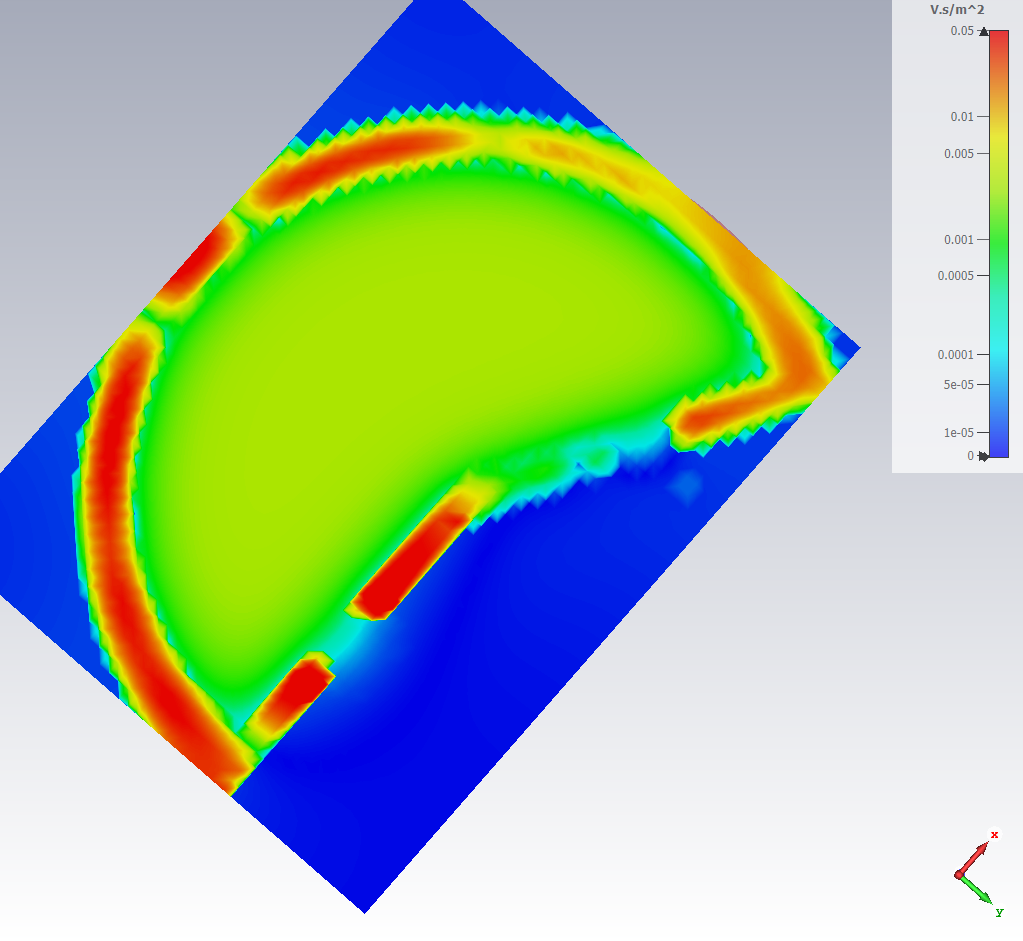
\includegraphics[width=.8\linewidth]{./figures/cst/cst_first_magnet_design3.png}
    \caption{Magnetic field in acceleration plate of initial magnet design.}
    \label{fig:initial_magnet_design_B}
\end{figure}
\fromfig{initial_magnet_design_B} shows that this design provides relatively uniform magnetic field inside, although magnetic field gradient in the openings can be improved. 

After adding two more magnets and using $\gamma=15^\circ$, the following second prototype design was created
\begin{figure}[H]
    \centering
    \captionsetup{justification=centering}
    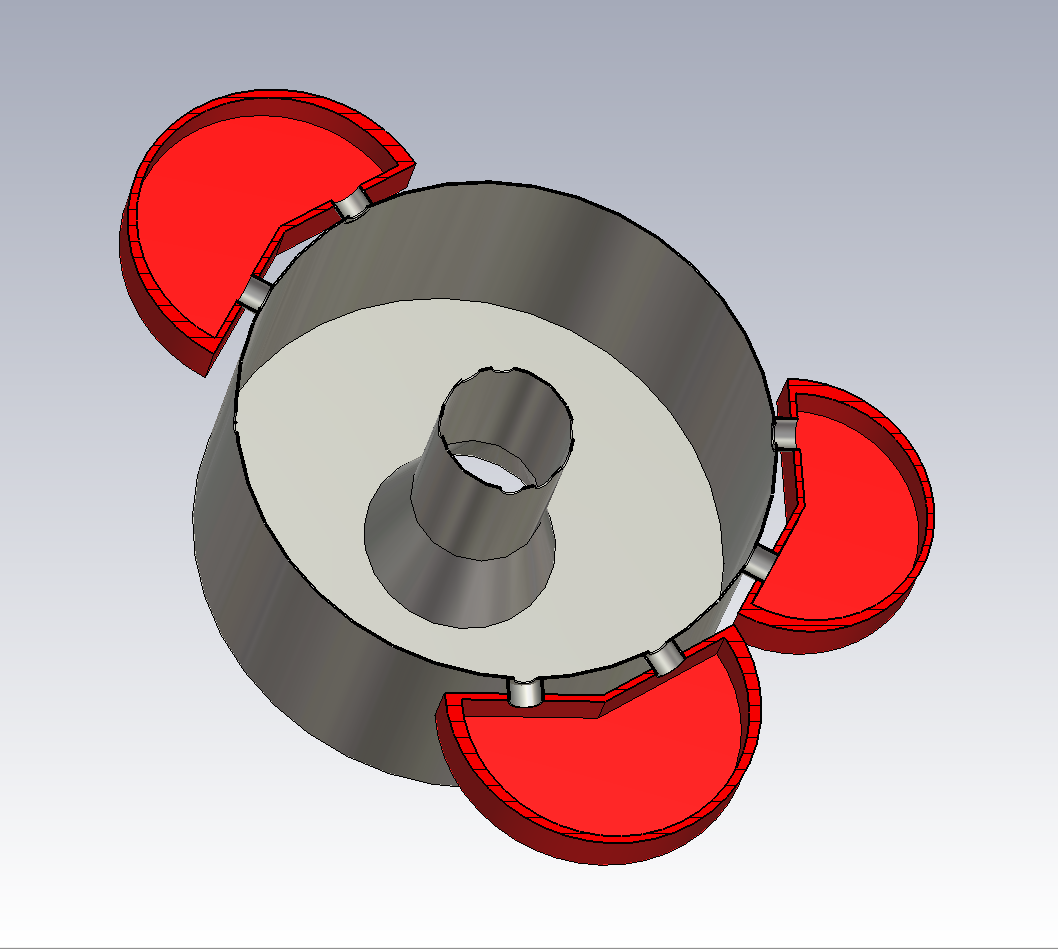
\includegraphics[width=.8\linewidth]{./figures/cst/cst_second_design2.png}
    \caption{Initial cavity with three magnets as shown in \fromfig{initial_magnet_design} \\ $\gamma=15^\circ$}
    \label{fig:initial_three_magnet_design}
\end{figure}
These designs, together with $40$ keV $e^-$ gun injecting with phase lag of $15^\circ$ for $1$ ns, was simulated at RF power of $12$ kW using \textit{CST Studio Particle Module PIC Solver}.
Results of these simulations can be found in \fromfig{initial_designs_PIC_phase_space_monitor}.
\begin{figure}[H]
    \captionsetup[subfigure]{justification=centering}
    \captionsetup{justification=centering}
    \centering
    \begin{subfigure}[b]{.8\textwidth}
      \centering
      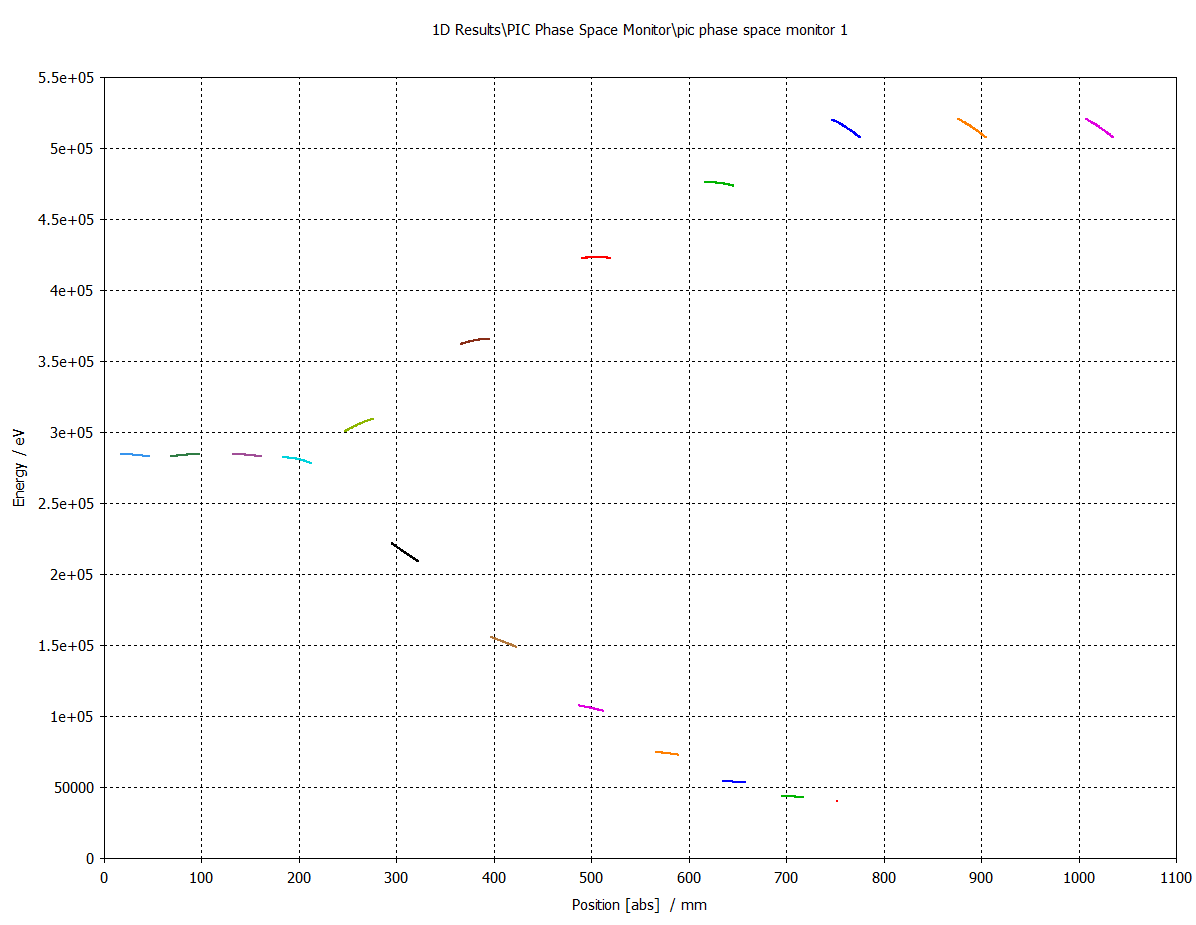
\includegraphics[width=\linewidth]{./figures/cst/cst_first_design4.png}
      \caption{One pass simulation of \fromfig{initial_design}}
    \end{subfigure}
    \centering
    \begin{subfigure}[b]{.8\textwidth}
      \centering
      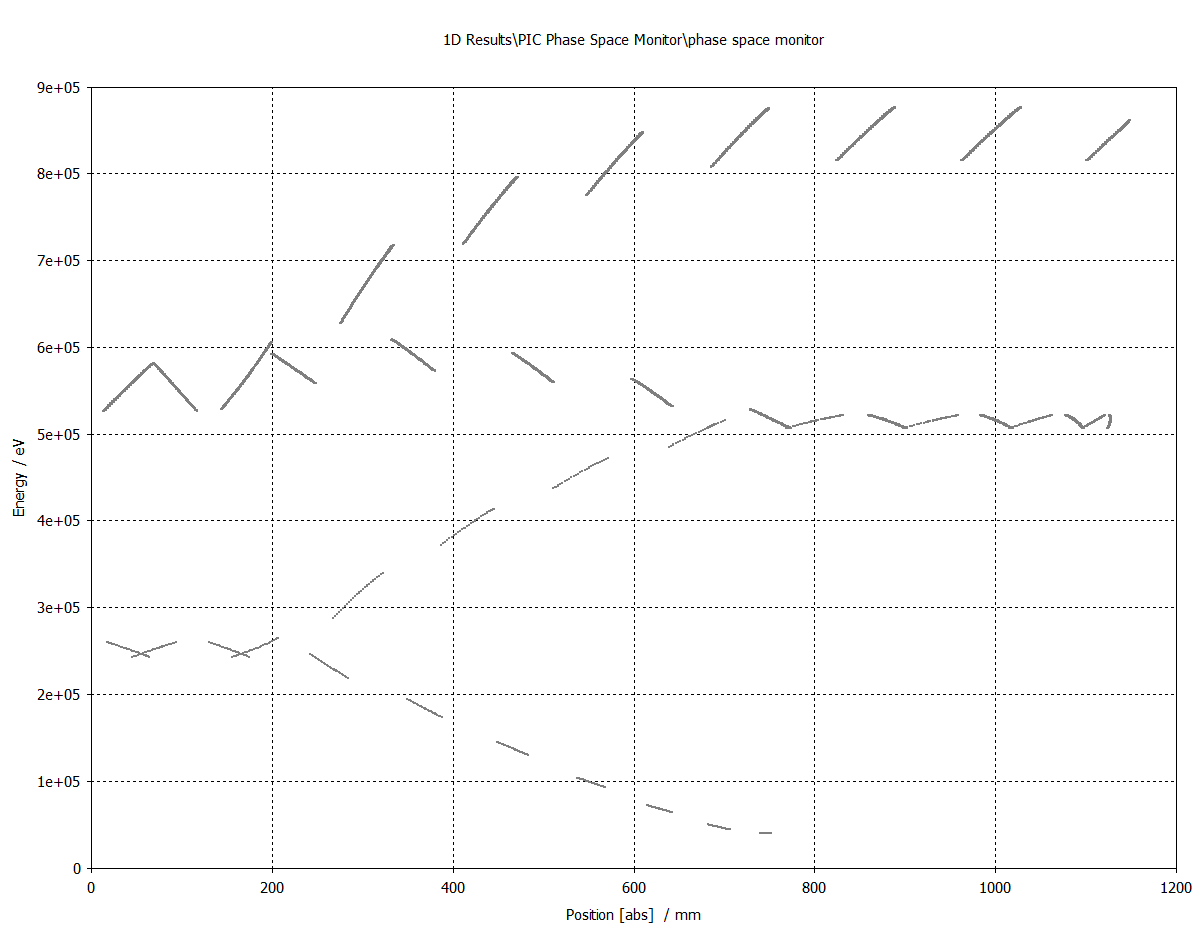
\includegraphics[width=\linewidth]{./figures/cst/cst_second_design3.png}
      \caption{Two pass simulation of \fromfig{initial_three_magnet_design}}
    \end{subfigure}
    \caption{$|r|$ vs $Energy$ simulation of initial design.}
    \label{fig:initial_designs_PIC_phase_space_monitor}
\end{figure}
The behavior of the beam in the \fromfig{initial_designs_PIC_phase_space_monitor} after the first pass indicates that phase stability is not maintained. 
When the simulation results are examined further, it was observed that the beam started the second pass at $t \approx 12$ ns after the injection. 
Considering the starting phase lag $\phi_{lag}=15^\circ$, this would mean phase lag of the second pass was $\phi_{lag2}=120^\circ$.
This result can be observed in \fromfig{initial_designs_PIC_phase_space_monitor}, as the beam decelerates after a short acceleration in the beginning of the second pass.

After various similar observations in \textit{CST} similations, underlying cause of this problem was thought to be the $L_{pass} = n \lambda$ approach on magnet design failing in low energies, 
as anticipated and discussed earlier in the \fromsec{parameter_sweep}.
\emph{The necessity for an alternative tool, capable of aiding researchers in improving beam behavior, was deemed evident.}

Several improvements were made to KAHVELab Rhodotron initial designs \cite{sinan}. These include curved edges on cavity which reduce the power loss on cavity walls, and redesigned iron casing on magnets for ease of production and maintenance.
Improved designs can be seen in the figures below.
\begin{figure}[H]
    \captionsetup[subfigure]{justification=centering}
    \captionsetup{justification=centering}
    \centering
    \begin{subfigure}{.5\textwidth}
      \centering
      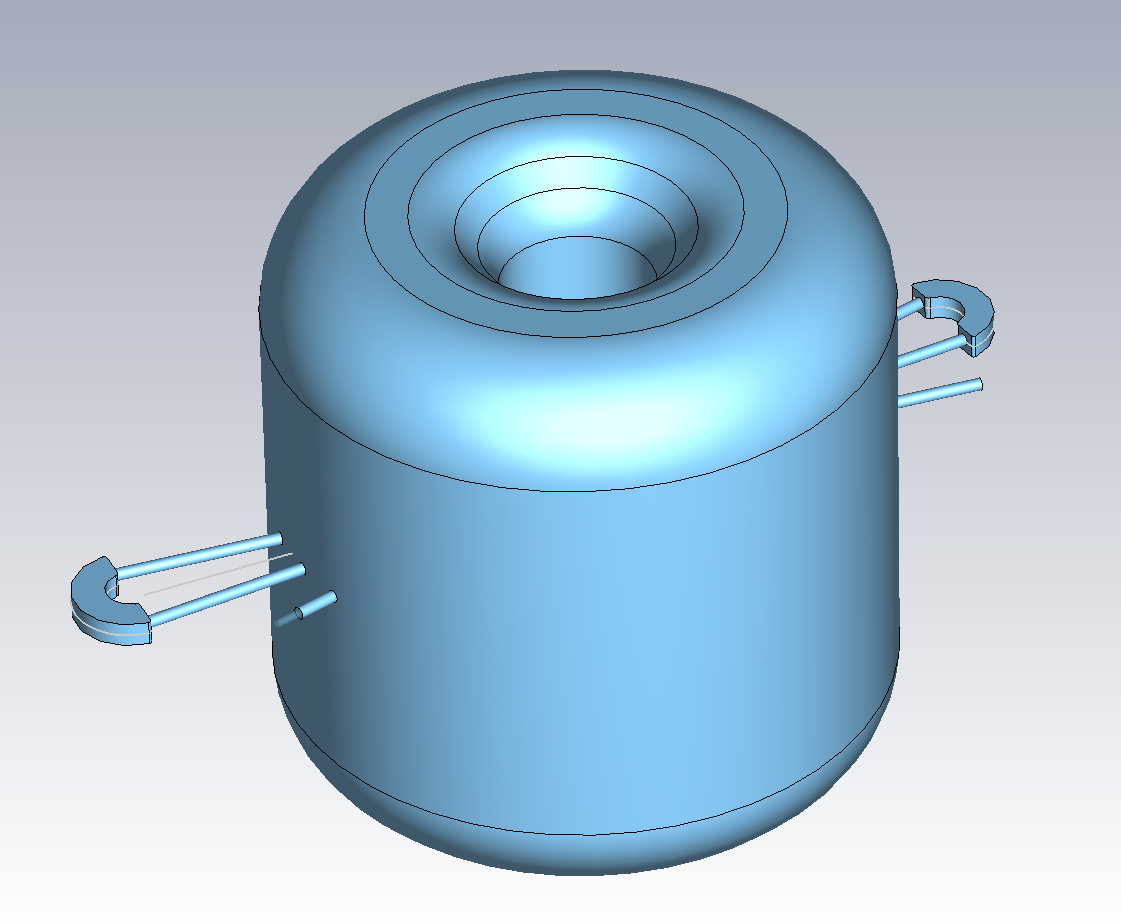
\includegraphics[width=.9\linewidth]{./figures/cst/cst_sinan_cavity_design1.png}
    \end{subfigure}%
    \centering
    \begin{subfigure}{.5\textwidth}
      \centering
      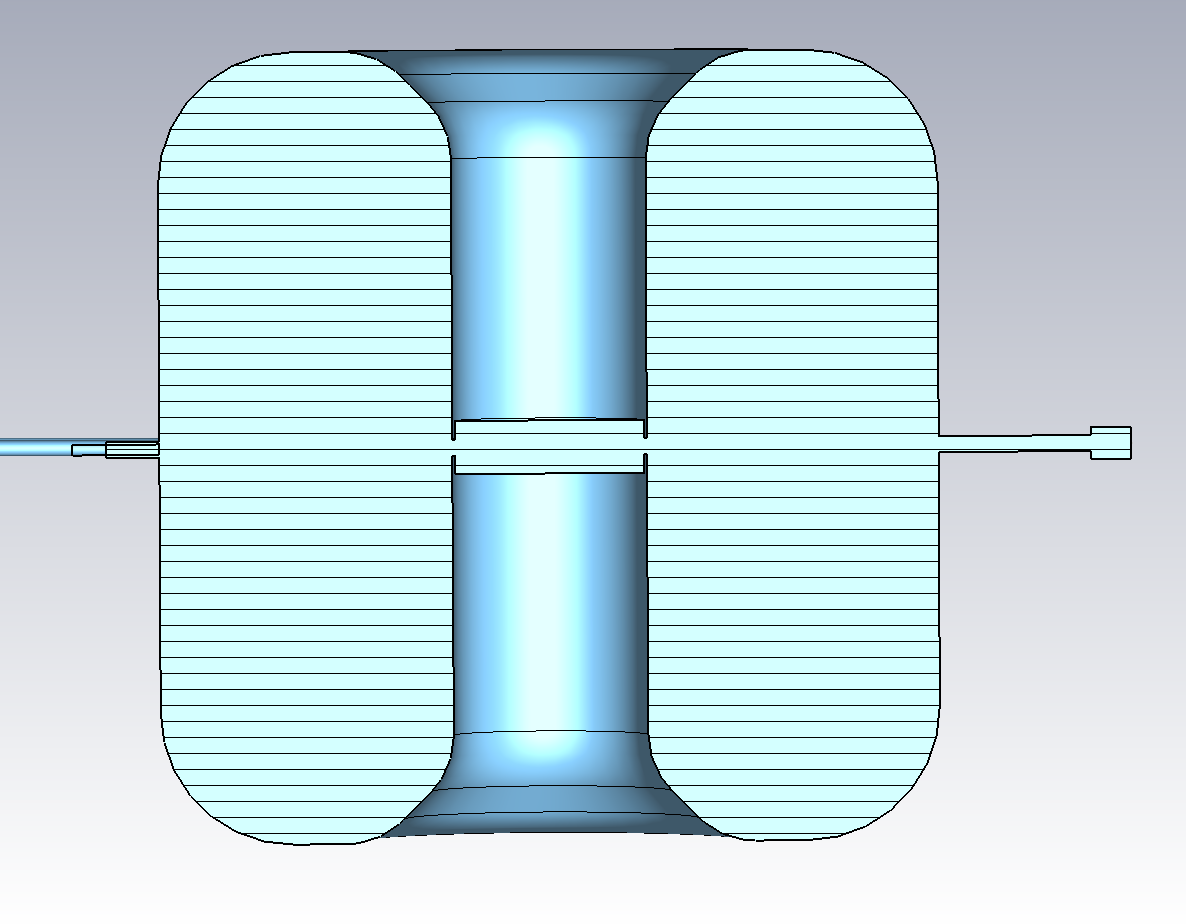
\includegraphics[width=.94\linewidth]{./figures/cst/cst_sinan_cavity_design2.png}
    \end{subfigure}
    \caption{Improved cavity design.}
    \label{fig:improved_cavity_design}
\end{figure}

\begin{figure}[H]
    \centering
    \captionsetup{justification=centering}
    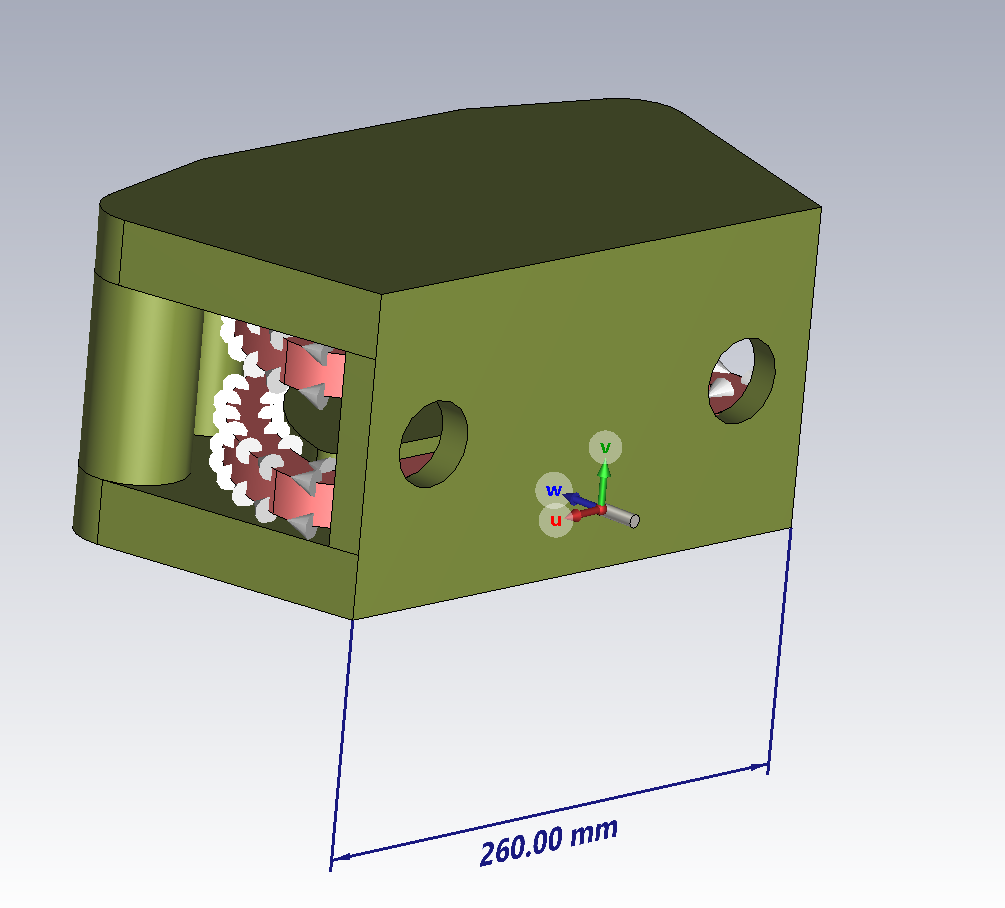
\includegraphics[width=.7\linewidth]{./figures/cst/cst_second_magnet_design1.png}
    \caption{Improved magnet design.}
    \label{fig:improved_magnet_design}
\end{figure}

\begin{figure}[H]
    \captionsetup[subfigure]{justification=centering}
    \captionsetup{justification=centering}
    \centering
    \begin{subfigure}{.5\textwidth}
      \centering
      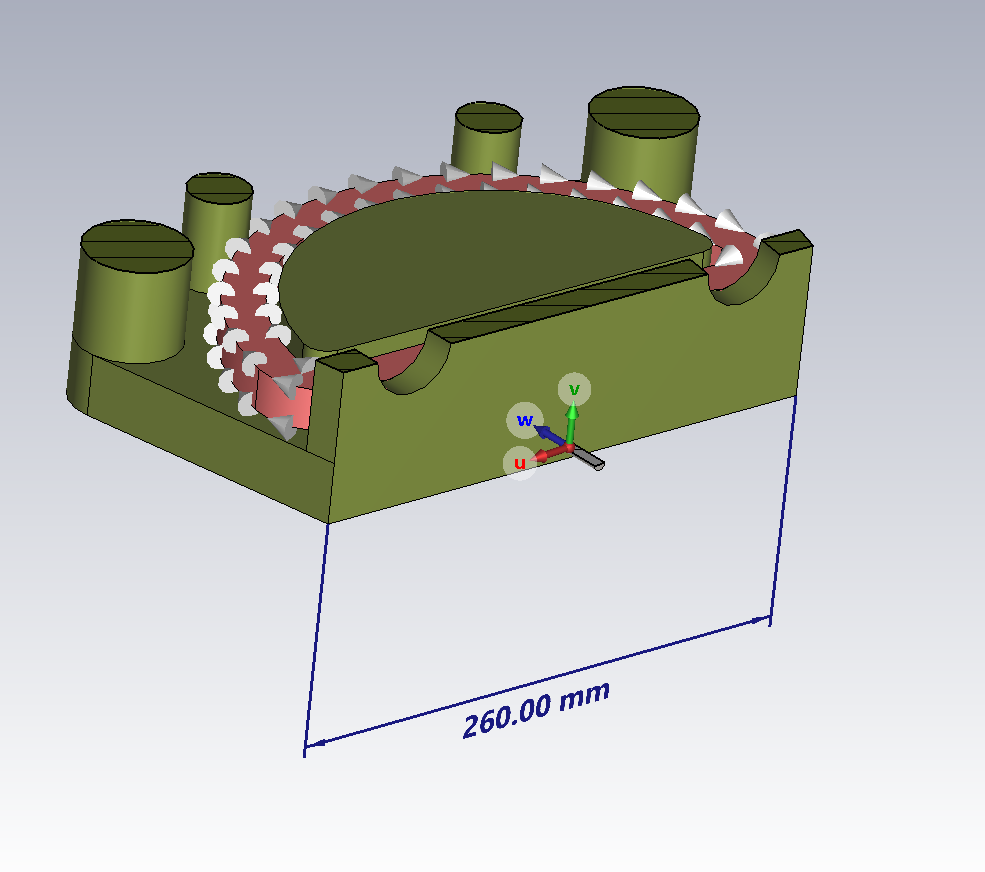
\includegraphics[width=.96\linewidth]{./figures/cst/cst_second_magnet_design2.png}
    \end{subfigure}%
    \centering
    \begin{subfigure}{.5\textwidth}
      \centering
      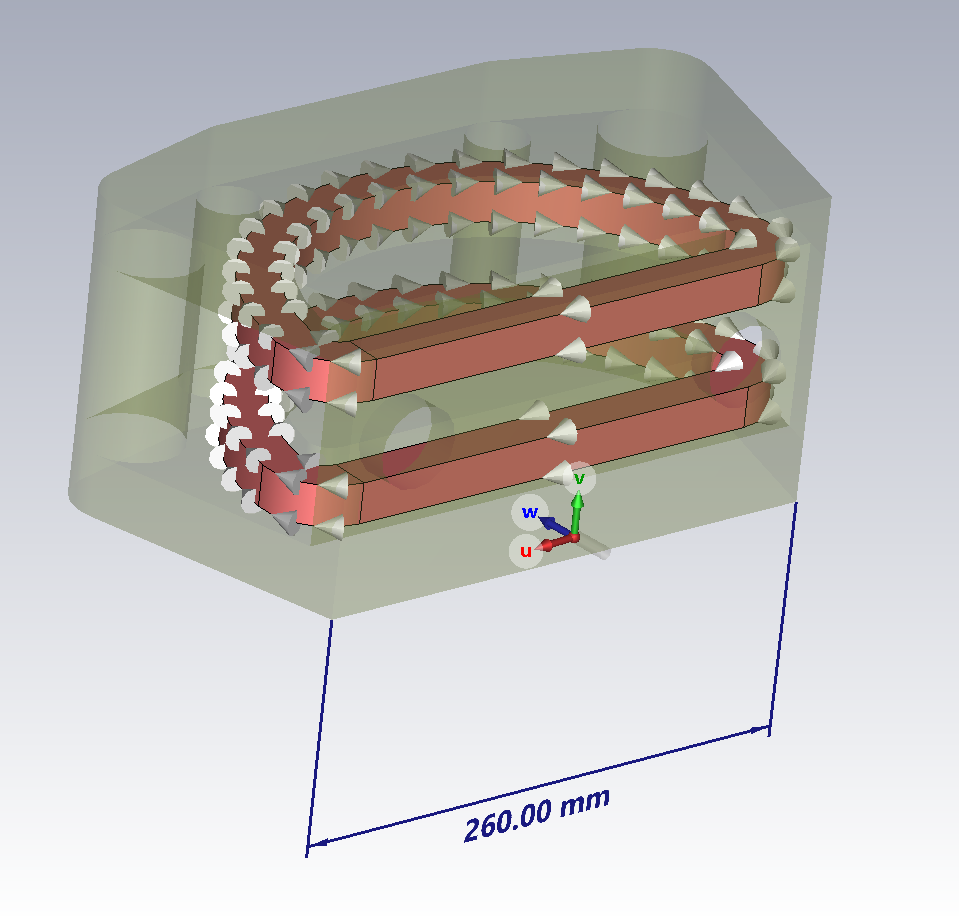
\includegraphics[width=.9\linewidth]{./figures/cst/cst_second_magnet_design3.png}
    \end{subfigure}
    \caption{Cross section and coils of improved magnet design.}
    \label{fig:improved_magnet_design_cross_section}
\end{figure}

\begin{figure}[H]
    \centering
    \captionsetup{justification=centering}
    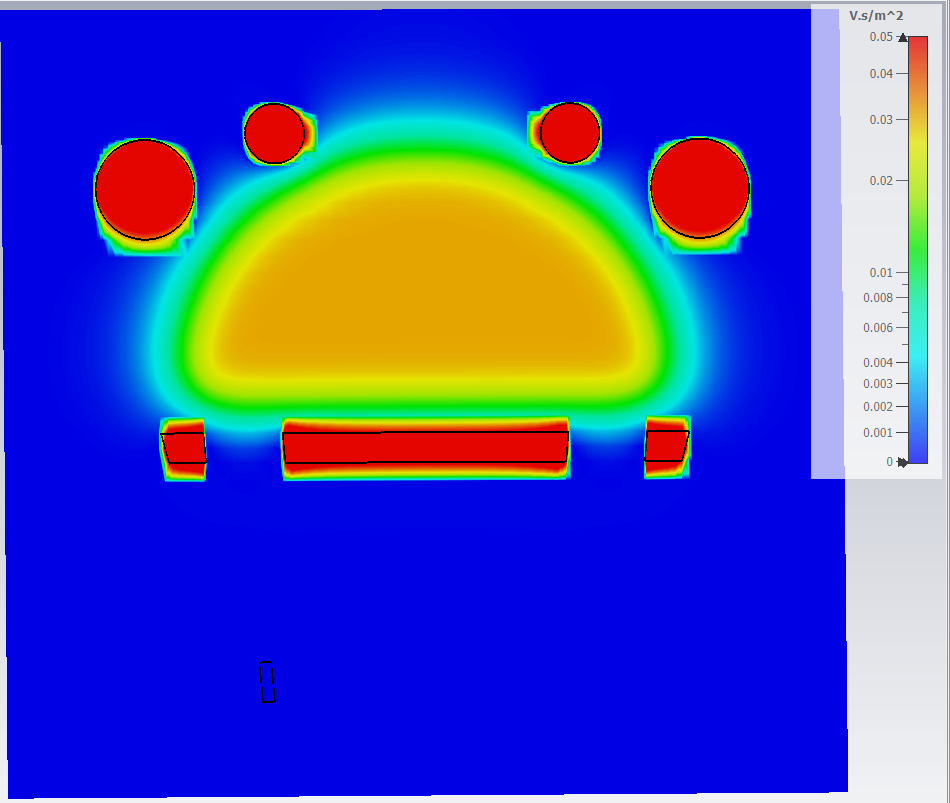
\includegraphics[width=.8\linewidth]{./figures/cst/cst_second_magnet_design4.png}
    \caption{Magnetic field in acceleration plate of improved magnet design.}
    \label{fig:improved_magnet_design_B}
\end{figure}
From \fromfigs{initial_magnet_design_B}{improved_magnet_design_B}, it can be observed that improved magnet design reduces magnetic field leak in enter and exit openings considerably. 
This reduction helps containing the spread of entering beam, decreasing the amount of focusing needed further into trajectory. 




\newpage

% START OF SIMULATION

\chapter{SIMULATION} \label{ch:simulation}

After considering the lack of design and simulation software available for \textit{Rhodotron-type} accelerators, 
together with the energy gain disagreement between \textit{CST Studio} and the calculations of \textit{J. Pottier} in \fromeq{W_gain_each_pass_pottier},
the need for a custom built tool became apparent. A simple 1D proof of concept was quickly implemented for this purpose.
% Start of poc.tex
\section{Proof of Concept}
The POC worked with interacting an electron with the EM field provided, at discrete time steps $dt$. The core sequence of this software is provided below.
Where $\vecthreeBF{r}$ is the position, $\vecthreeBF{v}$ is the velocity of the $e^-$;
\begin{itemize}
    \item Get electron energy $E_{in}$
    \item Get the RF field definitions
    \item Get the magnet design parameters if there is any
    \item Do following until the simulation time has ellapsed
    \begin{enumerate}
        \item Calculate $\vecthreeBF{E}_{||}$($\vecthreeBF{r}$)
        \item Calculate $\vecthreeBF{a}_{E ||}$ using \fromeq{para_and_perp_acc_of_lorentz_force}
        \item Calculate $\vecthreeBF{r}$($t+dt$) using \fromeq{leapfrog_sync_x}
        \item Calculate $\vecthreeBF{v}$($t+dt$) using \fromeq{leapfrog_sync_v}
        \item Calculate new $E_t$
    \end{enumerate}
\end{itemize}
The implemenation of this logic can be observed in \fromfig{POC_core_logic}. 
\begin{figure}[H]
    \begin{minted}[linenos=true, autogobble, frame=lines, framesep=2mm, fontsize=\footnotesize]{c++}
        for (double t=0; t<SimuTime; t+=dT){
            double RelBeta  = v/c;
            double RelGamma = 1.0 / sqrt(1.0-RelBeta*RelBeta);
        
            double ef=Eradial(r_pos*1000,t,0); // convert position to mm
            double acc=ef*1E6*eQMratio/(RelGamma*RelGamma*RelGamma); 
        
            r_pos = r_pos + v * dT*ns + 1/2*acc*(dT*ns)*(dT*ns);
            v = v + acc*dT*ns;

            RelBeta  = v/c;
            RelGamma = 1.0 / sqrt(1.0-RelBeta*RelBeta);
            Et=RelGamma*E0; 
        }
    \end{minted}
    \caption{Core logic loop of the POC}
    \label{fig:POC_core_logic}
\end{figure}
After simulating the \textit{synchronous electron} mentioned in \fromsec{cavity_of_a_rhodotron} with $\phi_{lag}=15^\circ$ for one pass, the results from \textit{POC}, \textit{CST} and \fromeq{W_gain_each_pass_pottier} are compared.
% 40 kW total power
% Emax = 0.96 in old, 2.08 in new version
% R1 = 0.1882
% R2 = 0.753
% f = 107.5
\begin{figure}[H]
    \begin{eqnarray}
        E_{Pottier} &=& 0.565 MeV \nonumber\\
        E_{CST} &=& 0.872 MeV  \label{eq:poc_E_results}\\
        E_{POC} &=& 0.873 MeV \nonumber
    \end{eqnarray}
    \caption*{$P=40$kW, $R_1=0.188$m, $R_2=0.753$m, $f=107.5$MHz}
\end{figure}
As can be observed in \fromeq{poc_E_results}, \textit{POC software} and \textit{CST} produced very similar results. However, we cannot make the same claim regarding \fromeq{W_gain_each_pass_pottier}.
This inconsistency between $E_{Pottier}$ and $E_{CST}$ was noticed in the earlier simulations as well, which supported the idea of using another simulation software to reduce reliance on \textit{CST}.
Since using a single software would have made the process error prone.

After the results obtained from \textit{POC} were found to be promising, a decision was made to develop a more robust simulation software. This software was named \textit{Rhodotron Simulation} for the current stage and started development in October, 2021.
The development and improvement efforts are still ongoing. 

During the development of \textit{Rhodotron Simulation} software, several intermediate builds have been implemented and tested. The following sections in this chapter investigates their implementations further.



% Start of intermediate.tex
\section{Intermediate Versions}

\subsection{$L_{out}$ Optimization For Single \e} \label{sec:lout_sweep}
Initial step of improving \textit{POC} towards \textit{Rhodotron Simulation} was to implement \textit{$L_{out}$ optimizations} to help optimazing magnet designs, as discussed in \fromsec{parameter_sweep}.
First approach was to hang the \e outside of the cavity for $t_{out} = L_{out}/v$, then inject it back to the cavity with reversed $\vecthreeBF{v}$. One can sweep the $t_{out}$ parameter to find the optimal value.
This simple implementation can be found in \fromfig{lout_opt_single_e} of \fromapp{intermediate_codes}.

Although the results from this optimization sweep were promising after they were simulated with $CST$, simulating one particle would not be sufficiently useful for designing a magnet.

\subsection{$\phi_{lag}$ Optimization For Bunches} \label{sec:philag_sweep}
After successfully accelerating single \e, particle bunches were implemented to approximate a real \e gun. 
They were modeled as $N$ electrons fired from an \e gun at even time intervals. This approach was taken because the amount of time gun fires, defined as \textit{Gun Active Time, $t_g$}, is a crucial part of pulsed \e gun design.

Addition of bunches would immediately proven useful when finding optimal phase lag for bunch entry.
$\phi_{lag}$ for a bunch was defined as the RF phase when the first \e of the bunch has entered the cavity and it defines the starting time of the current pass.
To use the \textit{parameter sweep} method, as used in \textit{$L_{out}$ optimization}, relevant bunch characteristics are defined as follows:
\begin{itemize}
    \item $\mu E$: Average energy
    \item $E_{rms}$: Root mean square of energy
    \item $R_{rms}$: Root mean square of \e positions
\end{itemize}
Optimal $\phi_{lag}$ would produce maximum $\mu E$ while minimizing $E_{rms}$ \& $R_{rms}$. For the first pass, 
$E_{rms}$ and $R_{rms}$ would be vaguely dependent of each other; therefore, initial implementation of $\phi_{lag}$ sweep was based on minimizing $E_{rms}$ during simulation (\textit{see \fromfig{phlag_opt}}). 
For $\mu E$ considerations, data from the software would be analyzed either manually or by using external tools such as \textit{ROOT framework}. 
\begin{figure}[H]
    \centering
    \captionsetup{justification=centering}
    \begin{minted}[linenos=true, autogobble, frame=lines, framesep=2mm, fontsize=\scriptsize]{c++}
        int phase_opt(int phase_sweep_range){
            double minrms = 1;
            int opt_phase;
            for(int RFphase = -phase_sweep_range; RFphase <= phase_sweep_range; RFphase++){
              Bunch bunch1(RFphase);
              double t1 = 0;
              bunch1.bunch_gecis_t(t1);
              bunch1.reset_pos();
        
              if( bunch1.E_rms() < minrms ){
                minrms = bunch1.E_rms();
                opt_phase = RFphase;
              }
            }
            return opt_phase;
        }
    \end{minted}
    \caption{$\phi_{lag}$ Optimization For Initial Bunch Design}
    \label{fig:phlag_opt}
\end{figure}
Since $\phi_{lag}$ is relatively easy to change after production, another version of \fromfig{phlag_opt} that was modified for given magnet design parameters was also implemented (\textit{see \fromfig{phlag_opt_n_pass} in \fromapp{intermediate_codes}}). 
This version can be useful for optimizing $\phi_{lag}$ in case of production issues in magnets. 

After the bunch and $\phi_{lag}$ sweep implementations, $L_{out}$ sweep was also updated to minimize $E_{rms}$. $\rho$ and $L$ calculations, using \fromeqs{magnet_rho_constraint}{magnet_L_constraint}, were also integrated. 
Two example runs from this intermediate build can be found in \fromfigs{lout_opt_1ns_Erms}{lout_opt_08ns_Erms} of \fromapp{example_simulation_runs}.

\subsection{Simulation in 3D}
After successfully implementing \eE interaction in 1D and confirming the usefulness of this tool, the decision was made to proceed with implementing a 3D version of the \textit{Rhodotron Simulation}.
Although complete refactoring of the software was necessary, this upgrade was crucial for implementation of \eB interaction.
The refactoring effort included proper implementation of \textit{OOP}, details of which can be seen in \fromfigsix{e_class}{bunch_class}{gun_class}{sim_class}{rhodosim_class}{rf_class} of \fromapp{intermediate_codes}.

Magnets were modeled as major segments of a circle, defined with $\vecthreeBF{r}_{mag}$, $\textbf{R}$ and $|\textbf{B}|$. 
For the initial implementation, $\vecthreeBF{B}$ assumed to be uniform and has no leaks outside the magnet boundary (\fromfig{is_inside_halfsphere} in \fromapp{intermediate_codes}).

Interaction logic for \eE and \eB in 3D can be found in \fromfig{3D_e_EM_interaction_first}.
\begin{figure}[H]
    \captionsetup[subfigure]{justification=centering}
    \captionsetup{justification=centering}
    \begin{subfigure}{\textwidth}
        \begin{minted}[linenos=true, autogobble, frame=lines, framesep=2mm, fontsize=\scriptsize]{c++}
            vector3d CoaxialRFField::actOn(Electron& e){
                vector3d Efield = getField(e.pos);                          // Calculate E vector
                vector3d F_m = Efield*1E6*eQMratio;                         // Calculate F/m vector
                vector3d acc = (F_m - e.vel*(e.vel*F_m)/(c*c))/e.gamma();   // Calculate a vector
                return acc;
            }
        \end{minted}
    \end{subfigure}

    \begin{subfigure}{\textwidth}
        \begin{minted}[linenos=true, autogobble, frame=lines, framesep=2mm, fontsize=\scriptsize]{c++}
            vector3d MagneticField::actOn(Electron& e){
                if (isInside(e.pos) == -1)
                    return vector3d(0,0,0);
                vector3d Bfield = getField(e.pos);                          // Calculate B vector
                vector3d F_m = (e.vel % Bfield)*eQMratio;                   // Calculate F/m vector
                vector3d acc = (F_m)/e.gamma();                             // Calculate a vector
                return acc;
            }
        \end{minted}
    \end{subfigure}
    \caption{\eEM  interaction logic from \fromeq{acc_of_E_and_B}}
    \label{fig:3D_e_EM_interaction_first}
\end{figure}
Where * and \% are, dot-product and cross-product respectably. (\fromfig{vector3d_dot_cross_product} of \fromapp{intermediate_codes})

Simulating in 3D had one other benefit; it was now possible to visualize the results by rendering the interaction data. 
For this purpose, \textit{gnuplot} was integrated into \textit{Rhodotron Simulation} to produce 2D visualization of acceleration plane. 
Rendered results could be stored as \textit{gif} animations. 
Two of such renders can be seen in \fromfig{example_gnuplot_renders}.
\begin{figure}[H]
    \captionsetup[subfigure]{justification=centering}
    \captionsetup{justification=centering}
    \centering
    \begin{subfigure}{0.9\textwidth}
        \centering
        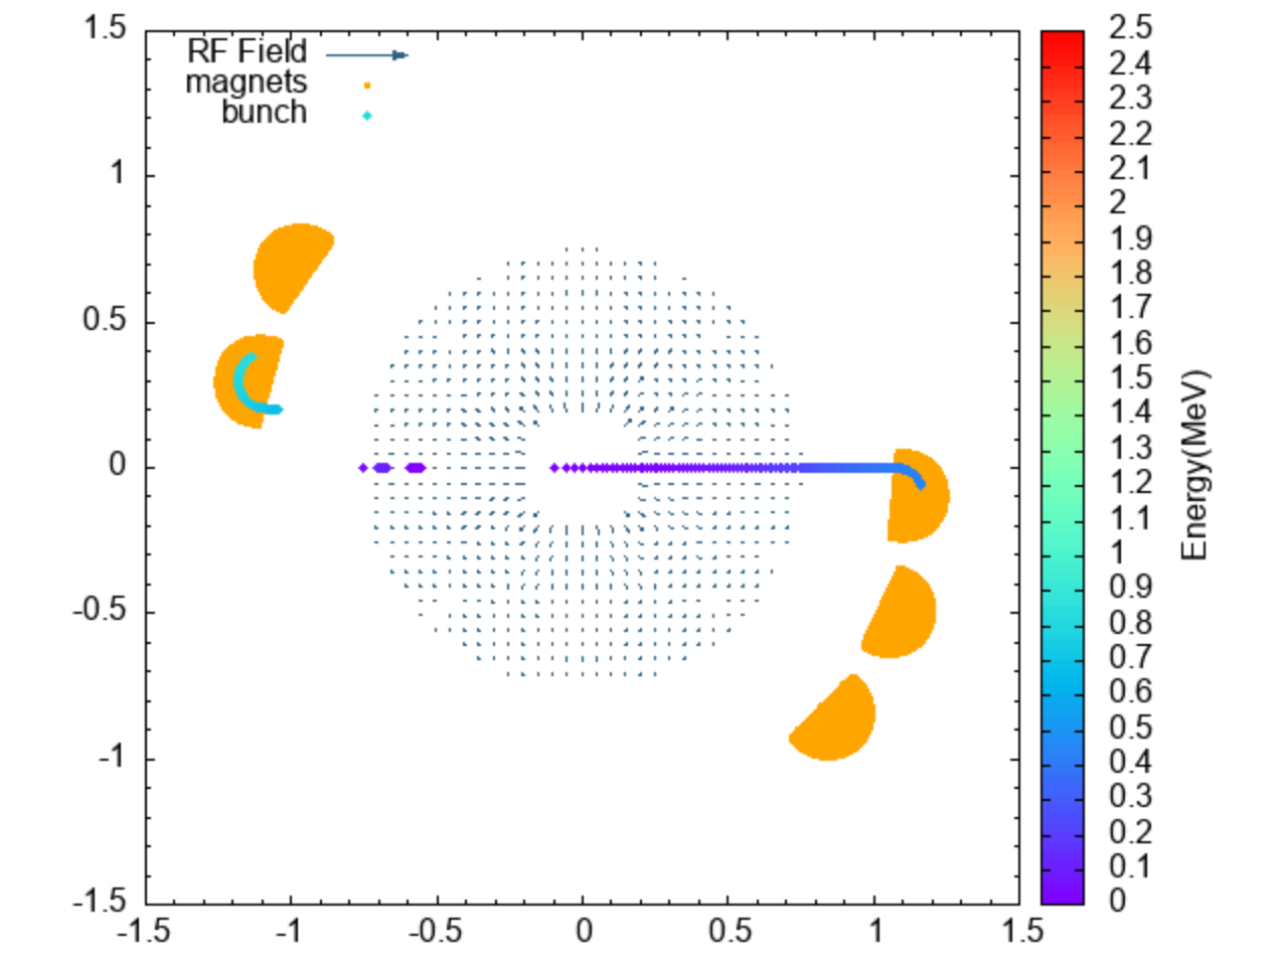
\includegraphics[width=\linewidth]{./figures/rhodoSim/5ns_gnuplot.png}
        \caption*{Unsyncronized \e gun period, $T_g = 5ns$}
    \end{subfigure}
    \begin{subfigure}{0.9\textwidth}
        \centering
        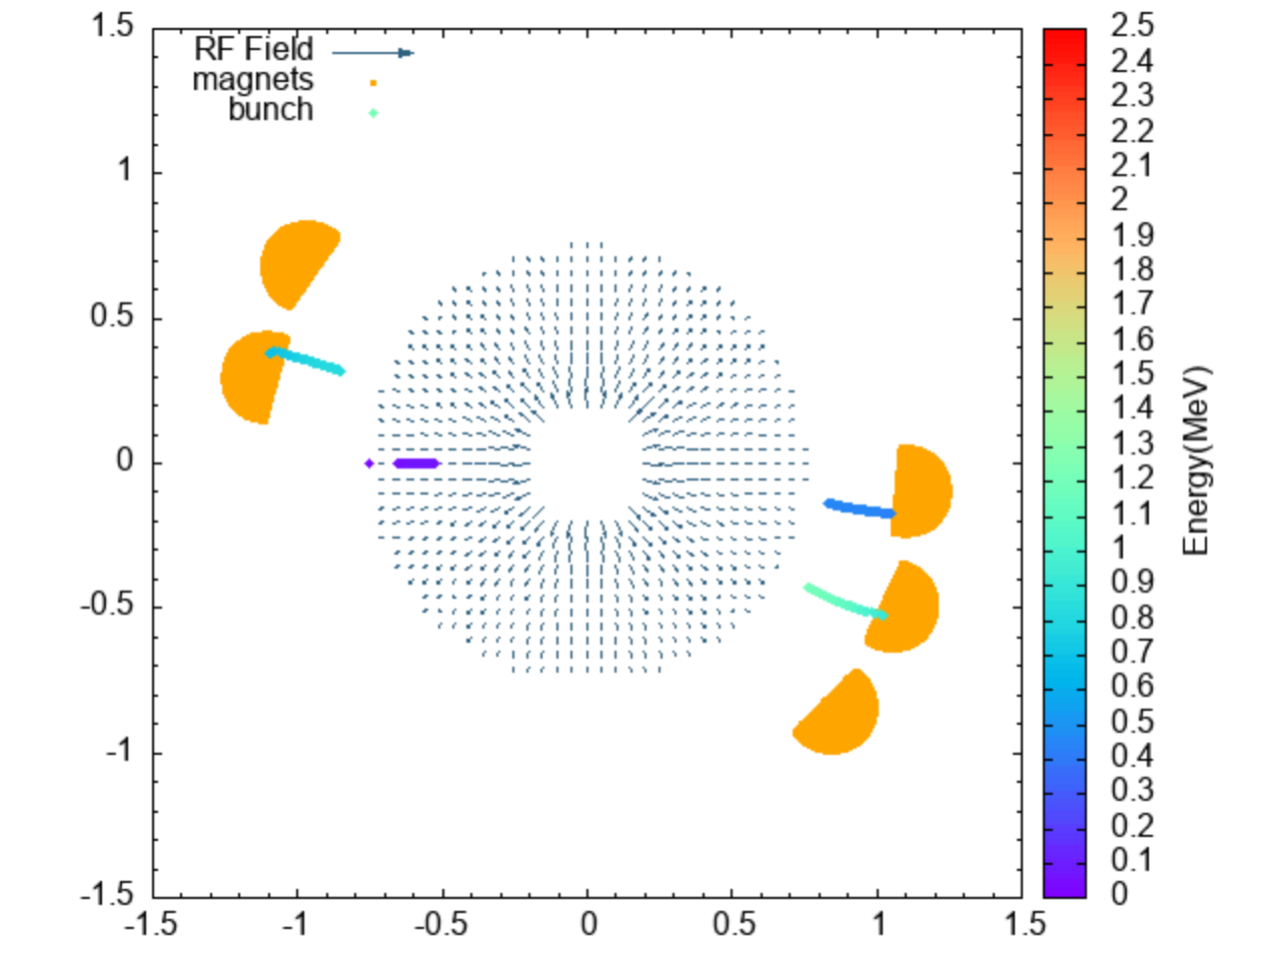
\includegraphics[width=\linewidth]{./figures/rhodoSim/9_3ns_gnuplot.png}
        \caption*{Syncronized \e gun period, $T_g = 9.3ns$}
    \end{subfigure}
    \caption{Example \textit{gnuplot} renders of \textit{Rhodotron Simulation}\\$P=12$kW, $f=107.5$MHz}
    \label{fig:example_gnuplot_renders}
\end{figure}

\subsection{Acceleration in Magnetic Field}
An issue regarding the \eB interaction became apparent when energy gain during these interactions was observed.
A setup simulation was implemented in which a bunch of 100\e at $1$MeV was fired into a uniform magnetic field of $0.1$T located in $x>0.05$m.
Initial results at $dt=0.01$ns proved the suspicion of \eB interaction being broken. However, the energy gain would decrease tremendously as $dt$ decreased.
\begin{figure}
    \captionsetup[subfigure]{justification=centering}
    \captionsetup{justification=centering}
    \centering
    \begin{subfigure}{0.8\textwidth}
        \centering
        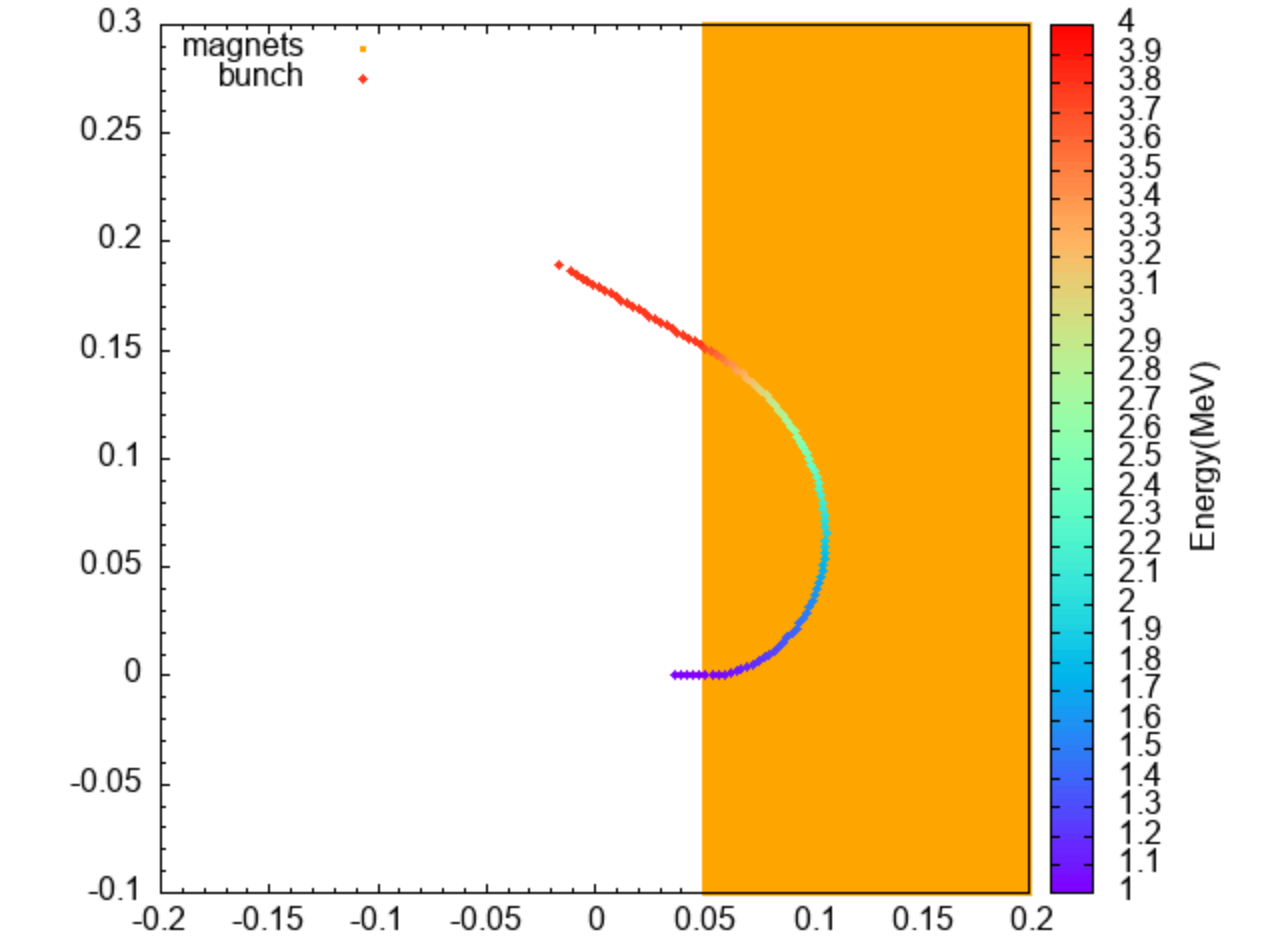
\includegraphics[width=\linewidth]{./figures/rhodoSim/mag_lf_001dt.png}
        \caption*{$dt=10^{-2}$ns, $\Delta E=2.783$MeV}
    \end{subfigure}
    \begin{subfigure}{0.8\textwidth}
        \centering
        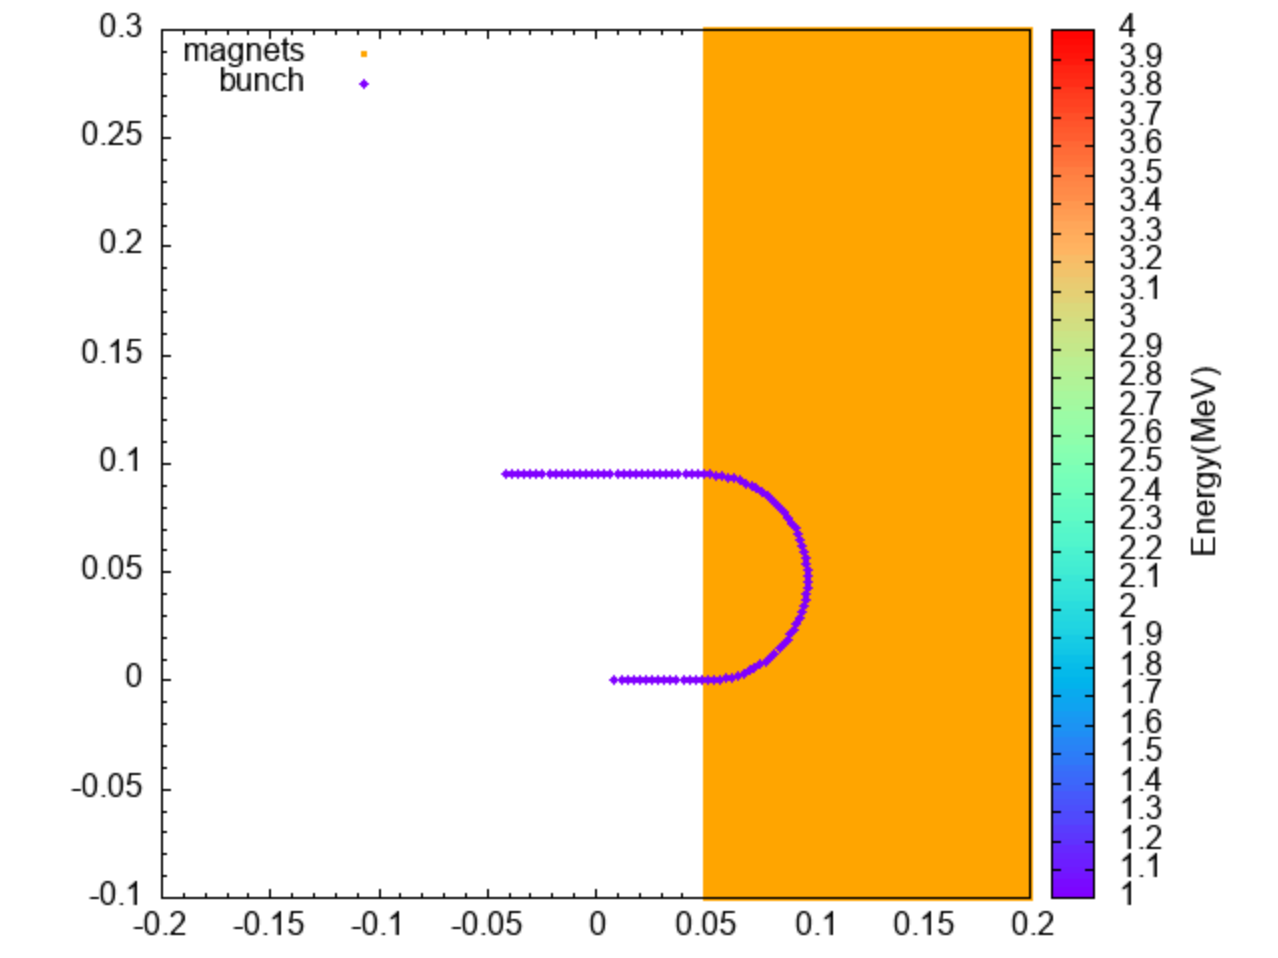
\includegraphics[width=\linewidth]{./figures/rhodoSim/mag_lf_00001dt.png}
        \caption*{$dt=10^{-4}$ns, $\Delta E=0.011$MeV}
    \end{subfigure}
    \caption{Energy gain of $1$MeV bunch in \textbf{B}=$0.1$T}
    \label{fig:mag_lf_render}
\end{figure}
Decreasing $dt$ would be the best way to increase accuracy of the results; however, this is not sustainable due to computing power limitations. 
Until this point, \textit{Rhodotron Simulation} have been using \fromsec{leapfrog} for \eEM interactions. 
To test newer approaches, two additional version of  \eEM interaction that are using \fromsec{rungekutta} were added.
\subsubsection{RK4-1}
First approach for integrating \fromsec{rungekutta} into \eEM interaction was to calculate $\vecthreeBF{a}_{E}$ and $\vecthreeBF{a}_{B}$ from \fromeq{acc_of_E_and_B} using \textit{RK4}.
After $\vecthreeBF{a}_{EM} = \vecthreeBF{a}_{E} + \vecthreeBF{a}_{B}$ was calculated, \e would move and accelerate using the \textit{Leap-frog} method. 
The idea was to produce more refined interaction results, leading to improved accuracy especially in \eB.
RF field was kept static during the RK4 computation, due to ongoing \textit{multithreading} implementation efforts. 
The implementation can be found in \fromfigs{rk1_B}{rk1_EM}.
\subsubsection{RK4-2}
Following the implementation of \textit{RK4-1}, revisions were made to the integration method for \textit{RK4} to replace \textit{Leap-frog}.
Instead of calculating $\vecthreeBF{a}_{EM}$ using \textit{RK4}, $\vecthreeBF{r}$ and $\vecthreeBF{v}$ would be determined directly.

These three methods were then tested in the same setup as \fromfig{mag_lf_render}. The results can be found in \fromfig{lf_rk1_rk2_comparison} of \fromapp{data_graph}.
\textit{RK4-1} was decided to be abandoned as it produced the same accuracy in twice the simulation time of \textit{RK4-2}.

More rigerous testing was done with \textit{Leap-frog} and \textit{RK4-2} however. 
Still using the setup in \fromfig{mag_lf_render}, each $dt$ configuration was simulated 10 times, calculating average and standard deviations afterwards.
Results from these tests can be observed in \fromfig{mag_lf_rk2_comparison}.
\begin{figure}
    \captionsetup[subfigure]{justification=centering}
    \captionsetup{justification=centering}
    \centering
    \begin{subfigure}{0.8\textwidth}
        \centering
        \includegraphics[width=\linewidth]{./figures/analiz/mag_lf_rk2_dt-E.png}
        \caption*{$dt$ vs $\Delta E$}
    \end{subfigure}
    
    \begin{subfigure}{0.8\textwidth}
        \centering
        \includegraphics[width=\linewidth]{./figures/analiz/mag_lf_rk2_dt-Tsim.png}
        \caption*{$dt$ vs $T_{sim}$}
    \end{subfigure}
    \caption{Comparing Leap-frog, RK4-2 performance on \eB interaction\\ $E_{in}=1$MeV, \textbf{B}=$0.1$T, $t_{end}=5$ns}
    \label{fig:mag_lf_rk2_comparison}
\end{figure}
The data from these tests can be found in \fromtabs{lf_mag_table}{rk2_mag_table} of \fromapp{data_graph}.
To investigate the data further, one can define a performance measurement, $F$.
\begin{eqnarray*}
    F &\propto& 1/T \\
    F &\propto& 1/\Delta E 
\end{eqnarray*}
When $dt=10^{-5}$ ns was taken as reference point due to providing a good balance of accuracy and computational intensity,
\begin{eqnarray} \label{eq:f_lf_rk_mag_1}
    \Delta E_{LF} &=& 110 \times 10^{-5} MeV \nonumber\\
    \Delta E_{RK}^1 &=& 64 \times 10^{-5} MeV \nonumber\\
    T_{LF}^1 &=& 9.44 \pm 0.03 s \nonumber\\
    T_{RK}^1 &=& 21.33 \pm 0.02 s \nonumber\\
    \Delta E_{LF} \times T_{LF} &=& 104 \times 10^{-4} \pm 10^{-4} MeV s \nonumber\\ %0.003
    \Delta E_{RK} \times T_{RK} &=& 137 \times 10^{-4} \pm 2\times 10^{-4}  MeV s \nonumber\\ %0.001
    F_{LF}/F_{RK} &=& \frac{\Delta E_{RK} \times T_{RK} }{\Delta E_{LF} \times T_{LF}^1} = 1.32 \pm 0.01
\end{eqnarray}
Also, observing from the data,
\begin{eqnarray} \label{eq:f_lf_rk_mag_2}
    \Delta E_{LF} (dt=3 \times 10^{-5}) \approx \Delta E_{RK} (dt=5 \times 10^{-5}) &\approx& 32.5 \times 10^{-4} MeV \nonumber\\
    T_{LF}(dt=3 \times 10^{-5})  &=& 3.18 \pm 0.02 s \nonumber\\ %0.0032
    T_{RK}(dt=5 \times 10^{-5})  &=& 4.30 \pm 0.01 s \nonumber\\ %0.0022
    F_{LF}/F_{RK} = \frac{T_{RK}(dt=5 \times 10^{-5})}{T_{LF}(dt=3 \times 10^{-5})} &=& 1.4 \pm 0.1
\end{eqnarray}
Uncertainty of \fromeq{f_lf_rk_mag_2} was taken high due to the approximation. After combining \fromeqs{f_lf_rk_mag_1}{f_lf_rk_mag_2}, $F$ can be calculated as
\begin{equation}
    F_{LF}/F_{RK} = 1.36 \pm 0.05
\end{equation}
Therefore, \textit{Leap-frog} was found to be the better choice as it provided with $1.36 \pm 0.05$ times accuracy in \eB interactions at a given time with respect to \textit{RK4}. However,
\textit{RK4} was promising in situations where decreasing the stepsize, $dt$, is not viable. Therefore both were integrated into \textit{Rhodotron Simulation} for the user to decide.
\textit{RK4-2} renders from these test can be found in \fromfig{mag_rk_render} of \fromapp{example_simulation_runs}.

\subsection{Acceleration in Electric Field}
After the accuracy concerns regarding the \eB interaction were raised, it was decided to test \eE and compare the performance of \textit{Leap-frog} and \textit{RK4}.

As test setups, two simulation confgurations were made. They aimed to test the accuracy of acceleration of a beam in parallel and perpendicular static uniform electric fields.
Both configurations had an \egun located at $(-0.753, 0, 0)$m, directed at $(1, 0, 0)$ firing electrons with the kinetic energy of $1$MeV. 
\begin{figure}[H]
    \centering
    \begin{subfigure}{0.47\textwidth}
        \centering
        \includegraphics[width=0.9\linewidth]{./figures/illustrations/statE_1.png}
        \caption*{Setup-1 parallel $\vecthreeBF{E}$ field}
    \end{subfigure}
    \begin{subfigure}{0.48\textwidth}
        \centering
        \includegraphics[width=0.9\linewidth]{./figures/illustrations/statE_2.png}
        \caption*{Setup-2, perpendicular $\vecthreeBF{E}$ field}
    \end{subfigure}
    \caption{Illustration of test setups.}
\end{figure}
In the first test, the beam would be injected into a static uniform electric field \\
$\vecthreeBF{E}=(-2.65616, 0, 0)$ MV/m where $-0.753<x<0.753$ and $-0.753<y<0.753$, $\vecthreeBF{E}=0$ elsewhere.

Considering the $\vecthreeBF{E}$ is parallel to the beam path, potential difference $V$ in the trejectory until \vecNum{-0.753}{0}{0}m is
\begin{eqnarray}
    \Delta V^1 &=& - \int \dotProdBF{E}{ds} \\
             &=& - \int_{-0.753}^{0.753} -2.65616 \times dx \\
             &=& 2.65616 \times 1.506 \\
    \Delta V^1 &=& 4 MV \\
    \Delta E^1 &=& 4 MeV \\
    E_{exitTH}^1 &=& 5 MeV
\end{eqnarray}
In the second test on the other hand, the beam would be injected into a different static uniform electric field, \\
$\vecthreeBF{E}=(0, -5.31232, 0)$ MV/m where $-0.753<x<0.753$ and $-0.753<y<0.753$, $\vecthreeBF{E}=0$ elsewhere.
\begin{eqnarray}
    \Delta V^2   &=& - \int \dotProdBF{E}{ds} \\
                 &=& - \int_{0}^{0.753} -5.31232 \times dy \\
                 &=& 5.31232 \times 0.753 \\
    \Delta V^2   &=& 4 MV \\
    \Delta E^2   &=& 4 MeV \\
    E_{exitTH}^2 &=& 5 MeV
\end{eqnarray}
Therefore, in the both tests, the beam was expected to exit $\vecthreeBF{E}$ with $E_{exitTH} = 5$ MeV. 
To also measure the variance in simulation completion times, $T_{sim}$, set of $10$ runs were completed at the configuration for each $dt$ value.
Results from these tests can be observed in \fromfig{lf_rk2_perp_stat_E_comparison} and \fromfig{lf_rk2_par_stat_E_comparison} of \fromapp{data_graph}.
\begin{figure}[H]
    \centering
    \begin{subfigure}{0.9\textwidth}
        \centering
        \includegraphics[width=\linewidth]{./figures/rhodoSim/statE_par.png}
        \caption*{Setup-1, $\textbf{V}_{\parallel}$=4MV}
    \end{subfigure}
    \begin{subfigure}{0.9\textwidth}
        \centering
        \includegraphics[width=\linewidth]{./figures/rhodoSim/statE_perp.png}
        \caption*{Setup-2, $\textbf{V}_{\perp}$=4MV}
    \end{subfigure}
    \caption{Render of the test setups. \\ $E_{in}=1$ MeV, $t_{end}=6$ ns}
\end{figure}

\begin{figure}[H]
    \captionsetup[subfigure]{justification=centering}
    \captionsetup{justification=centering}
    \centering
    \begin{subfigure}{0.9\textwidth}
        \centering
        \includegraphics[width=\linewidth]{./figures/analiz/90staticE_lf_rk2_dt-E_3.png}
    \end{subfigure}
    
    \begin{subfigure}{0.9\textwidth}
        \centering
        \includegraphics[width=\linewidth]{./figures/analiz/90staticE_lf_rk2_dt-Tsim.png}
    \end{subfigure}
    \caption{Comparing Leap-frog, RK4-2 performance on \eE interaction\\ $E_{in}=1$MeV, $\textbf{V}_{\perp}$=4MV, $t_{end}=6$ ns}
    \label{fig:lf_rk2_perp_stat_E_comparison}
\end{figure}
Taking the $dt=10^{-5}$ ns for the reference point as before, the relative performance can be calculated.
\begin{eqnarray*}
    \begin{aligned}
        \Delta E_{LF}^1 &=& 22 \times 10^{-6} MeV \\
        \Delta E_{RK}^1 &=& 16 \times 10^{-6} MeV \\
        T_{LF}^1 &=& 12.40 \pm 0.04 s \\
        T_{RK}^1 &=& 40.08 \pm 0.12 s \\
    \end{aligned}
    \qquad
    \begin{aligned}
        \Delta E_{LF}^2 &=& 15 \times 10^{-5} MeV \\
        \Delta E_{RK}^2 &=& 9.3 \times 10^{-5} MeV \\
        T_{LF}^2 &=& 10.75 \pm 0.04 s \\
        T_{RK}^2 &=& 34.93 \pm 0.39 s 
    \end{aligned}
\end{eqnarray*}

\begin{eqnarray} \label{eq:f_lf_rk_1}
    \Delta E_{LF}^1 \times T_{LF}^1 &=& 270 \times 10^{-6} \pm 10^{-6} MeV s \nonumber\\ %0.003
    \Delta E_{RK}^1 \times T_{RK}^1 &=& 640 \times 10^{-6} \pm 2\times 10^{-6}  MeV s \nonumber\\ %0.003
    F_{LF}^1/F_{RK}^1 &=& \frac{\Delta E_{RK}^1 \times T_{RK}^1 }{\Delta E_{LF}^1 \times T_{LF}^1} = 2.4 \pm 0.02
\end{eqnarray}

\begin{eqnarray} \label{eq:f_lf_rk_2}
    \Delta E_{LF}^2 \times T_{LF}^2 &=& 160 \times 10^{-5} \pm 10^{-5} MeV s \nonumber\\ %0.004
    \Delta E_{RK}^2 \times T_{RK}^2 &=& 320 \times 10^{-5} 4 \pm 10^{-5} MeV s \nonumber\\ %0.011
    F_{LF}^2/F_{RK}^2 &=& \frac{\Delta E_{RK}^2 \times T_{RK}^2 }{\Delta E_{LF}^2 \times T_{LF}^2} = 2.0  \pm 0.03
\end{eqnarray}
\textit{Leap-frog} provides $2.4$ times and $2.0$ times less overacceleration per simulation time than \textit{RK4} in parallel and perpendicular electric fields respectably.
This results can be tested further with obsering from the data (see \fromtabf{lf_statE_table}{rk2_statE_table}{lf_statE90_table}{rk2_statE90_table} of \fromapp{data_graph}),
\begin{eqnarray} \label{eq:f_lf_rk_3}
    \Delta E_{LF}^1 (dt=2 \times 10^{-5}) = \Delta E_{RK}^1 (dt=3 \times 10^{-5}) &=& 45 \times 10^{-6} MeV \nonumber\\
    T_{LF}^1(dt=2 \times 10^{-5})  &=& 6.23 \pm 0.02 s \nonumber\\ %0.0032
    T_{RK}^1(dt=3 \times 10^{-5})  &=& 13.40 \pm 0.03 s \nonumber\\ %0.0022
    F_{LF}^1/F_{RK}^1 = \frac{T_{RK}^1(dt=3 \times 10^{-5})}{T_{LF}^1(dt=2 \times 10^{-5})} &=& 2.15 \pm 0.02
\end{eqnarray}
\begin{eqnarray} \label{eq:f_lf_rk_4}
    \Delta E_{LF}^2 (dt=3 \times 10^{-5}) \approx \Delta E_{RK}^2 (dt=5 \times 10^{-5}) &\approx& 470 \times 10^{-6} MeV \nonumber\\
    T_{LF}^2(dt=3 \times 10^{-5})  &=& 3.62 \nonumber\\ %0.0055
    T_{RK}^2(dt=5 \times 10^{-5})  &=& 7.00 \nonumber\\ %0.0071 -> 0,0126
    F_{LF}^2/F_{RK}^2 = \frac{T_{RK}^2(dt=5 \times 10^{-5})}{T_{LF}^2(dt=3 \times 10^{-5})} &=& 1.9 \pm 0.1
\end{eqnarray}
The last uncertainty was taken high due to the approximation of $467 \approx 471$. After combining \fromeqsf{f_lf_rk_1}{f_lf_rk_2}{f_lf_rk_3}{f_lf_rk_4},
the performance of \textit{Leap-frog} relative to \textit{RK4} in \eE interaction can be calculated as in \fromeq{lf_rk_eE_relative_performance}.
\begin{equation}\label{eq:lf_rk_eE_relative_performance}
    F_{LF}/F_{RK} = 2.11 \pm 0.03
\end{equation}
Therefore, it can be concluded that \textit{Leap-frog} outperforms \textit{RK4} with the relative performance of $2.11 \pm 0.03$ in \eE interactions with static uniform $\vecthreeBF{E}$ field. 

\subsection{Multithreading}
As already mentioned before, multithreading implementation efforts were ongoing since right after the start of this project. 
There have been a number of different approaches for implementation. 
First implemenation was done when the \textit{Rhodotron Simulation} was only capable of 1D simulations.
After the sizable refactoring done for 3D capabilities, this implementation was obselete. 
\begin{figure}[H]
    \centering
    \includegraphics[width=\linewidth]{./figures/illustrations/multh_arc.png}
    \caption{An Illustration of the multithreading architecture.}
    \label{fig:multh_illustration}
\end{figure}
For the current version, a main thread that spawns and manages several other worker threads would be used as can be seen in \fromfig{multh_illustration}.
The UI-Console thread would handle incoming and outgoing communication, notifying the user about the status of simulation 
(see \fromfig{console_output_running} in \fromapp{example_simulation_runs} for example console notification, \fromfig{ui_thread} in \fromapp{intermediate_codes} for implemenation)
or communucating with the \textit{GUI} that will be disscussed in the next section.

Focus of this section is the worker threads, also known as \eEM interaction threads.
There were four competing architecture for these worker threads,
\begin{enumerate}
    \item Have a thread pool that calculates \eEM in a queue 
    \item Assign a thread to each bunch
    \item Assign random electrons to each thread and calculate \eEM with global time
    \item Assign random electrons to each thread and calculate \eEM with local thread time
\end{enumerate}
\textbf{Architecture 1} would require constant waiting in worker threads to get mutexes of $\vecthreeBF{E}$ field, especially in \textit{RK4}.

\textbf{Architecture 2} was performing well in configurations with a large number of bunches, but was not increasing performance in lower bunch count configurations as expected.

\textbf{Architecture 3} was inefficient and wasteful since all the worker threads would wait the main thread to get the next time after they finish calculation, while the main thread would be waiting for the slowest worker thread.

\textbf{Architecture 4} was thought to be the best performer. It would give freedom to calculate the whole simulation to each thread while giving up the global time.
This would also mean thread-safety is ensured since there is no shared data between the worker threads. 
However, this architecture can cause issues if \ee interactions were decided to be implemented in the future.

Another caveat is that a copy operation of $\vecthreeBF{E}$ and $\vecthreeBF{B}$ objects for each worker thread would be needed.
This would lead to larger memory allocations and more time spent setting up simulations. 
Therefore, \textit{Architecture 4} is not ideal for fast calculations and when the memory is an important constraint.
An implementation that can use both \textbf{Architecture 2} \& \textbf{Architecture 4} when necessary would be a better approach considering these methods;
nevertheless, \textbf{Architecture 4} was chosed to be implemented.

The implemenation can be found in \fromfigf{_runMT}{fireAllWithFireTimesMT}{setupPool}{threadLoop} in \fromapp{intermediate_codes}.



% Start of intermediate.tex
\section{Graphical User Interface}

\begin{figure}[H]
    \centering
    \includegraphics[width=\linewidth]{./figures/illustrations/RhodoSim_GUI_Draft_V02.pdf}
    \caption{An Illustration of the first GUI design.}
    \label{fig:gui_illustration}
\end{figure}
Until this point, \textit{Rhodotron Simulation} could be used with a configration file, defining the problem that would be simulated.
An example of this configuration file can be found in \fromfig{config_file} of \fromapp{example_simulation_runs}. 
This approach was simple and fast; however, it was not suitable for the average target user since required basic knowledge of command line interface and was not up to modern standards.
For this reason, a GUI was decided to be built, using \textit{ROOT framework}. 
This would also enable \textit{Rhodotron simulation} to make use of analysis tools offered by \textit{ROOT}.


The initial design of the \textit{Rhodotron Simulation GUI} can be observed in \fromfig{gui_illustration}.
\begin{figure}[h]
    \centering
    \includegraphics[width=\linewidth]{./figures/rhodoSim/GUI_config_frame.png}
    \caption{The configuration frame of implementated first GUI design.}
    \label{fig:gui_config}
\end{figure}
The \textit{GUI} would be a standalone application, running the \textit{Rhodotron Simulation} as a service when needed. 
For this reason, the now called \textit{simulation engine} was updated to be able to run as a background service of \textit{GUI}.
By this approach, one could also ignore the \textit{GUI} altogether and use the \textit{simulation engine} as before, as these are two seperate products.

In the \fromfig{gui_config}, the implemented version of \fromfig{gui_illustration} can be observed. This version of the \textit{GUI} has the following frames;

\subsection{Configuration Frame}
This frame provides an interface for specifying, saving or loading a configuration, consists of $\vecthreeBF{B}$ field, $\vecthreeBF{E}$ field, \textit{RF} description, \egun, \textit{simulation} configuration regions.
Each one having an illustration of what the parameters are as can be seen in \fromfig{gui_config}.

\subsection{Simulation Frame}
This frame spawns and manages the \textit{simulation engine}, configures and starts the simulation. 
It has a progress bar that shows the current progress of the simulation, communucating with \textit{UI handler thread} in \textit{simulation engine}.
Simulation frame while a simulation is running can be observed in \fromfig{gui_simulate_1} of \fromapp{supp}.

\subsection{Render Frame}
Since the rendering capabilities of \textit{ROOT} is superior than \textit{gnuplot}, the user can render a playback of the simulation in real time, 
see a specific time frame, export as snapshot or animated gif file.
Two example renders can be seen in \fromfig{gui_render_1} and \fromfig{gui_render_2} of \fromapp{supp}.
\begin{figure}
    \centering
    \includegraphics[width=\linewidth]{./figures/rhodoSim/GUI_render_frame_5.png}
    \caption{Render frame of \textit{GUI}.}
    \label{fig:gui_render_1}
\end{figure}

\subsection{Analyze Frame}
Analyze frame provides tools for analyzing and visualizing the simulation data. 
In the current version, \textbf{E} distribution histogram and \textbf{E(t)} graph of each electron are implementated into this frame.
This frame is a work in progress and will be the focus of improvement and become a really powerfull tool in the near future.
In \fromfig{gui_analyze_Edist}, \textit{Analyze Frame} plotting \textbf{E} distribution histogram, and in \fromfig{gui_analyze_Et} and \fromfig{gui_analyze_Et2} of \fromapp{supp}, \textit{Analyze Frame} plotting \textbf{E(t)} graphs can be observed.
\begin{figure}
    \centering
    \includegraphics[width=\linewidth]{./figures/rhodoSim/GUI_analyze_Edist_2.png}
    \caption{Analyze frame of \textit{GUI} E distribution.}
    \label{fig:gui_analyze_Edist}
\end{figure}

\begin{figure}
    \centering
    \includegraphics[width=\linewidth]{./figures/rhodoSim/GUI_analyze_Et_3.png}
    \caption{Analyze frame of \textit{GUI} E(t).}
    \label{fig:gui_analyze_Et}
\end{figure}


\subsection{Sweep Frame}
Parameter sweep method that was discussed in \fromsecs{lout_sweep}{philag_sweep} was integrated into \textit{GUI} in a seperate frame named \textit{Sweep Frame}.
$\phi_{lag}$ sweep was the first parameter to be implemented. 

It takes the range of sweep, draws $\phi_{lag}$ vs $\mu E$, $\phi_{lag}$ vs $\sigma E$ and $\phi_{lag}$ vs $\sigma R$ mentioned in \fromsec{philag_sweep}.
This enables user with an already built accelerator to optimize \egun parameters quickly. 
In the \fromfigf{gui_sweep_muE}{gui_sweep_sE}{gui_sweep_running}{gui_sweep_sR} of \fromapp{supp}, this frame can be inspected in detail.

\begin{figure}
    \centering
    \includegraphics[width=\linewidth]{./figures/rhodoSim/GUI_sweep_muE_3.png}
    \caption{Sweep frame of \textit{GUI} \\ $\phi_{lag}$ $\mu E$ result.}
    \label{fig:gui_sweep_muE}
\end{figure}
\begin{figure}
    \centering
    \includegraphics[width=\linewidth]{./figures/rhodoSim/GUI_sweep_sE_3.png}
    \caption{Sweep frame of \textit{GUI} \\ $\phi_{lag}$ sweep $\sigma E$ result.}
    \label{fig:gui_sweep_sE}
\end{figure}

As mentioned before, \textit{GUI} is the latest and ongoing development effort in this project.
New analysis and sweep features will be implemented and current capabilities will be improved in the near future.



\newpage

% START OF PRODUCTION

\chapter{PRODUCTION}

As discussed before, production efforts of a \textit{Rhodotron-type} accelerator are still ongoing in KAHVELab.
This accelerator will be used at $f=107.5$MHz $P=50-100$kW to achieve beams with the energy range of $1-5$MeV.
% Start of final.tex
\section{Final Design} \label{sec:final_design}
In the following figures, rendered visuals of the final design can be observed \cite{sinan}.
\begin{figure}[H]
    \centering
    \includegraphics[width=\linewidth]{./figures/design/final_design_in_lab.JPG}
    \caption{Rhodotron in KAHVELab}
\end{figure}

\begin{figure}
    \centering
    \includegraphics[width=\linewidth]{./figures/design/final_design_1.png}
    \caption{Rhodotron cavity and \e gun}
\end{figure}

\begin{figure}
    \centering
    \includegraphics[width=\linewidth]{./figures/design/final_design_2.png}
    \caption{Vertical cross section of the beam injection line}
\end{figure}

\begin{figure}
    \centering
    \includegraphics[angle=90, origin=c, width=\linewidth]{./figures/design/final_design_3.png}
    \caption{Cross section of the acceleration plane}
\end{figure}


% Start of techd.tex
\section{Technical Drawing}
Technical drawings of the design mentioned in \fromsec{final_design} can be found in \fromfigs{techd_rhod}{techd_mid}, \fromfig{techd_up} of \fromapp{supp}.
\begin{figure}
    \centering
    \includegraphics[angle=270,origin=c, width=.98\linewidth]{./figures/teknikcizim/Rho-A1.0.00.pdf}
    \caption{Technical drawing of the rhodotron cavity. \cite{sinan}}
    \label{fig:techd_rhod}
\end{figure}

\begin{figure}
    \centering
    \includegraphics[angle=270,origin=c, width=\linewidth]{./figures/teknikcizim/Rhodotron Elektron Hizlandirici Sistemi.pdf}
    \caption{Technical drawing of middle part of the cavity which contains the beam line. \cite{sinan}}
    \label{fig:techd_mid}
\end{figure}

% Start of mani.tex
\section{Manifacturing}

Manifacturing of the rhodotron cavity has been ongoing, planned to be completed in the following months.

The cavity itself was manifactured as 5 main parts, using 5mm thick stainless steel sheet. 

Elastic version of the 304, 304L was chosen to be the production material for ease of bending.
These sheets were then pressed to achieve the shapes of the parts. 
Several flanges were then machined, including
\begin{itemize}
    \item $4.5$in EIA RF flange for RF input
    \item ISO100-KF vacuum connector flanges for vacuum pumps
    \item ISO-63 KF flange for probe insertion
    \item KF40 flanges for beam line vacuum gauges
\end{itemize}
After desired shapes were produced inside surface of the sheets were polished with 2000 grits. 
304 stainless steel sheet bars of different sizes were then added by 
TIG welding to achieve pressure resistance.

Because the main body of the cavity was 5mm thick and 304L was used, deformations on cylinderical symmetry were encountered. 
This problem was solved by welding 6 10mm thick toroidal sheets between the coaxial cylinders, 
which would be removed after the heat treatment.
\begin{figure}
    \captionsetup[subfigure]{justification=centering}
    \captionsetup{justification=centering}
    \centering
    \begin{subfigure}{.5\textwidth}
      \centering
      \includegraphics[width=.96\linewidth]{./figures/manif/polish/rhodo_bottom_unpolished_cropped.jpeg}
      \caption{Bottom part of the cavity while polishing.}
    \end{subfigure}%
    \centering
    \begin{subfigure}{.5\textwidth}
      \centering
      \includegraphics[width=.96\linewidth]{./figures/manif/polish/rhodo_upper_polished_cropped.jpeg}
      \caption{Top part of the cavity after polishing.}
    \end{subfigure}
    \caption{Polishing of the inner surface of cavity.}
    \label{fig:manif_polishing}
\end{figure}


\begin{figure}
    \captionsetup[subfigure]{justification=centering}
    \captionsetup{justification=centering}
    \centering
    \begin{subfigure}{.5\textwidth}
      \centering
      \includegraphics[width=.96\linewidth]{./figures/manif/toroidal_sheets/rhodo_bottom_cropped.jpeg}
      \caption{Bottom part of the cavity with the exposed beam line in inner cylinder.}
    \end{subfigure}%
    \centering
    \begin{subfigure}{.5\textwidth}
      \centering
      \includegraphics[width=.96\linewidth]{./figures/manif/toroidal_sheets/rhodo_middle_toroidal_sheets_welded_cropped.jpeg}
      \caption{Bottom part of the cavity with the beam line assembled.}
    \end{subfigure}
    \caption{Deformation prevention measure, 10 mm thick toroidal sheets.}
    \label{fig:manif_toroidal_sheets}
\end{figure}

\begin{figure}
    \captionsetup{justification=centering}
    \centering
    \includegraphics[width=.8\linewidth]{./figures/manif/welding/rhodo_middle_sheetbars_cropped.jpeg}
    \caption{Welded sheet bars.}
\end{figure}

\begin{figure}
    \captionsetup{justification=centering}
    \centering
    \includegraphics[width=.7\linewidth]{./figures/manif/toroidal_sheets/rhodo_middle_only_cropped.jpeg}
    \caption{Middle part of the cavity containing the beam line.}
\end{figure}


\begin{figure}
    \captionsetup[subfigure]{justification=centering}
    \captionsetup{justification=centering}
    \centering
    \begin{subfigure}{.5\textwidth}
      \centering
      \includegraphics[width=.96\linewidth]{./figures/manif/welding/rhodo_assembled_welding_cropped.jpeg}
      \caption{Welding sheet bars.}
    \end{subfigure}%
    \centering
    \begin{subfigure}{.5\textwidth}
      \centering
      \includegraphics[width=.96\linewidth]{./figures/manif/welding/rhodo_middle_welding_toroidal_sheets_cropped.jpeg}
      \caption{Welding toroidal sheets.}
    \end{subfigure}
    \caption{TIG welding.}
    \label{fig:manif_welding}
\end{figure}

\begin{figure}
    \captionsetup[subfigure]{justification=centering}
    \captionsetup{justification=centering}
    \centering
    \begin{subfigure}{.5\textwidth}
      \centering
      \includegraphics[width=.96\linewidth]{./figures/manif/assembled/rhodo_assembled_2_cropped.jpeg}
    \end{subfigure}%
    \centering
    \begin{subfigure}{.5\textwidth}
      \centering
      \includegraphics[width=.96\linewidth]{./figures/manif/assembled/rhodo_assembled_1_cropped.jpeg}
    \end{subfigure}
    \caption{Assembled cavity as the current stage.}
    \label{fig:manif_assembled}
\end{figure}




% Start of rf.tex
% \section{RF Supply}




\newpage

% START OF FUTURE_WORK

\chapter{CONCLUSION}
At the time of publication, production efforts of a new rhodotron type electron accelerator are currently continuing in KAHVELab. 
Present bottleneck is the fabrication of the cavity.

\section{Future Work}
Regarding the cavity manufacturing process, it is in the concluding stages.
The sheet bars and the flanges of the upper and the lower parts have been produced and are being welded and getting ready for heat treatment.
After the heat treatment operation, 
the supporting toroidal sheets will be removed and the inside surface will be polished before cyanide copper plating. 

As far as the magnets concerned, it was decided to be kept on hold in the early stages of the project, 
due to the disagreement on energy gain amount between the calculations of \textit{J. POTTIER} \cite{rhodo_pottier} 
and the simulation results from \textit{CST Studio Suite} \& \textit{Rhodotron Simulation}. 
The software is planned to be used in magnet design and beam optimizations in KAHVELab after the initial tests are completed.

\textit{Rhodotron Simulation}, which has been the main focus of this thesis, is ready and waiting to be tested with the cavity that is being manufactured; 
several improvements and new feature implementations are underway in the mean time. 
They include the following;
\begin{figure}[H]
    \begin{subfigure}[t]{0.5\textwidth}
        \begin{itemize}
            \item Electric and magnetic field import
            \item Field generator module to directly produce field files from specified cavity
            \item Synchrotron radiation calculations to determine radiation and energy loss
            \item \ee interactions
            \item Redesign of the GUI
            \item 3D render in GUI
        \end{itemize}
    \end{subfigure}
    \begin{subfigure}[t]{0.5\textwidth}
        \begin{itemize}
            \item Refactoring of the \eEM interaction and logging to improve performance
            \item Refactoring of the GUI Render Frame to improve render speed
            \item Refactoring the magnet class to introduce field leaks
            \item Extention of analysis tools in Analyze Frame
            \item $L_{out}$ sweep in Sweep Frame
        \end{itemize}
    \end{subfigure}
\end{figure}
After the cavity manufacturing is concluded, energy gain predictions of this software will be tested on this cavity. 
Complementary bending magnet design will be the first challange of \textit{Rhodotron Simulation}, which will provide tremendous testing and improvement opportunities.

\section{Discussion}
In conclusion, a new computational \eEM interaction simulation and analysis tool that focuses on designing and improving \textit{Rhodotron-type} accelerators has been successfully developed; 
a \textit{Rhodotron-type} accelerator with an operating frequency of $107.5$ MHz and a target energy of $1-5$ MeV has been designed and is currently being manufactured.

The software features a robust GUI that is capable of rendering and analyzing simulation results.
Leap-frog and Runge-Kutta numerical methods have been implemented for initial speed and accuracy tests.
The real-world performance and accuracy of this new tool, on the other hand, cannot be tested
before the cavity production is completed and the performance is compared with the predictions of the tool;
however, the capabilities it presents, coupled with the analogous results obtained from other extensively utilized simulation tools, 
lead to the inference that it holds promise.

\newpage


\appendix
\chapter{Intermediate Codes} \label{appendix:intermediate_codes}
\begin{figure}[H]
    \centering
    \captionsetup{justification=centering}
    \begin{subfigure}{\textwidth}
        \centering
        \begin{minted}[linenos=true, autogobble, frame=lines, framesep=2mm, fontsize=\scriptsize]{c++}
            for(double i = 2; i < 9; i += dT_out){
                t_dum += i;
                double enow = gecis(r_pos, vel, Et, t_dum);
                if( enow > maxE ){
                  maxE = enow;
                  t_opt = i;
                }
                t_dum = t;
            }
        \end{minted}
    \end{subfigure} 
    \\
    \begin{subfigure}{\textwidth}
        \centering
        \begin{minted}[linenos=true, autogobble, frame=lines, framesep=2mm,  fontsize=\scriptsize]{c++}
            double gecis(double r_pos, double vel, double Et, double &t){
                for(; r_pos >= -R2 && r_pos <= R2 ; t+=dT){
                    vel = c*sqrt(Et*Et-E0*E0)/Et;
                    double RelBeta  = vel/c;
                    double RelGamma = 1.0 / sqrt(1.0-RelBeta*RelBeta);
                
                    double ef=Eradial(r_pos*1000,t,RFphase*deg_to_rad);
                
                    double acc=ef*1E6*eQMratio/(RelGamma*RelGamma*RelGamma); 
                
                    r_pos = r_pos + vel * dT*ns + 1/2*acc*(dT*ns)*(dT*ns);
                    vel=vel+acc*dT*ns;
                    RelBeta  = vel/c;
                    RelGamma = 1.0 / sqrt(1.0-RelBeta*RelBeta);
                    Et=RelGamma*E0; 
                }
                return Et;
            }
        \end{minted}
    \end{subfigure}
    \caption{$L_{out}$ Optimization For Single \e}
    \label{fig:lout_opt_single_e}
\end{figure}

\begin{figure}[H]
        \centering
        \captionsetup{justification=centering}
        \begin{minted}[linenos=true, autogobble, frame=lines, framesep=2mm, fontsize=\scriptsize]{c++}
            int phase_opt(const vector<double>& Louts, int phase_sweep_range){
                double minrms = 1;
                int opt_phase;
                for(int RFphase = -phase_sweep_range; RFphase <= phase_sweep_range; RFphase++){
                    Bunch bunch1(RFphase);
                    double t1 = 0;
                    bunch1.bunch_gecis_t(t1);
                    bunch1.reset_pos();
            
                    for(int i = 0; i < Louts.size(); i++){
                        bunch1.bunch_gecis_d(Louts[i]);
                        bunch1.reset_pos();
                    }
                        
                    if( bunch1.E_rms() < minrms ){
                        minrms = bunch1.E_rms();
                        opt_phase = RFphase;
                    }
                }
                return opt_phase;
            }
        \end{minted}
    \caption{$\phi_{lag}$ Optimization For Initial Bunch Design}
    \label{fig:phlag_opt_n_pass}
\end{figure}

\begin{figure}[H]
    \captionsetup[subfigure]{justification=centering}
    \captionsetup{justification=centering}
    \begin{subfigure}{\textwidth}
        \begin{minted}[linenos=true, autogobble, frame=lines, framesep=2mm, fontsize=\scriptsize]{c++}
            double vector3d::operator* (const vector3d& other){
                double dot = 0;
                dot += this->x * other.x;
                dot += this->y * other.y;
                dot += this->z * other.z;
                return dot;
            }
        \end{minted}
    \end{subfigure}

    \begin{subfigure}{\textwidth}
        \begin{minted}[linenos=true, autogobble, frame=lines, framesep=2mm, fontsize=\scriptsize]{c++}
            vector3d vector3d::operator% (const vector3d& other){
                double x_ = (this->y * other.z) - (this->z * other.y);
                double y_ = (this->z * other.x) - (this->x * other.z);
                double z_ = (this->x * other.y) - (this->y * other.x);
                vector3d crossed(x_, y_, z_);
                return crossed;
            }
        \end{minted}
    \end{subfigure}
    \caption{* and \% operators of \textit{vector3d} class}
    \label{fig:vector3d_dot_cross_product}
\end{figure}

\begin{figure}[H]
    \centering
    \captionsetup{justification=centering}
    \begin{minted}[linenos=true, autogobble, frame=lines, framesep=2mm, fontsize=\scriptsize]{c++}
        bool isInsideHalfSphere(vector3d e_position, double r, vector3d hs_position){
            vector3d relative = e_position - hs_position;       
            // r/5 can be changed, use this for now                                
            if ( relative.magnitude() <= r && relative * hs_position.direction() >= -r/5){      
                return true;                                                                 
            }
            return false;
        }
    \end{minted}
\caption{Logic of is \e inside the shape of magnet}
\label{fig:is_inside_halfsphere}
\end{figure}

\begin{figure}[H]
    \centering
    \captionsetup{justification=centering}
    \begin{minted}[linenos=true, autogobble, frame=lines, framesep=2mm, fontsize=\scriptsize]{c++}
        vector3d Electron2D::interactB_RK(const MagneticField& B, double time_interval){
            if (B.isInside(pos) == -1){
                return vector3d(0,0,0);
            }
            Electron2D e_dummy;
            e_dummy.Et = Et;
            e_dummy.pos = pos;
            e_dummy.vel = vel;
            double time_halved = time_interval*0.5;
            // get k1                                       
            vector3d F_m = (e_dummy.vel % B.getField(pos))*eQMratio;                                       
            vector3d k1 = F_m * e_dummy.gamma_inv();     
            // get k2
            e_dummy.move(time_halved);
            e_dummy.accelerate(k1, time_halved);                                              
            F_m = (e_dummy.vel % B.getField(pos))*eQMratio;                                               
            vector3d k2 = F_m * e_dummy.gamma_inv();    
            // get k3
            e_dummy.vel = vel;
            e_dummy.accelerate(k2, time_halved);
            vector3d k3 = F_m * e_dummy.gamma_inv();   
            // get k4
            e_dummy.vel = vel;
            e_dummy.move(time_halved);
            e_dummy.accelerate(k3, time_interval);                                           
            F_m = (e_dummy.vel % B.getField(pos))*eQMratio;  
            vector3d k4 = F_m * e_dummy.gamma_inv();
        
            return (k1 + k2*2 + k3*2 + k4)/6;
        }
    \end{minted}
\caption{RK4-1 implemenation of \e-$\vecthreeBF{B}$}
\label{fig:rk1_B}
\end{figure}
\begin{figure}[H]
    \centering
    \captionsetup{justification=centering}
    \begin{minted}[linenos=true, autogobble, frame=lines, framesep=2mm, fontsize=\scriptsize]{c++}
        void Electron2D::interactRK_ActorE(const RFField& E, const MagneticField& B, double time_interval){
            vector3d run_kut_E = interactE_RK(E, time_interval);
            vector3d run_kut_B = interactB_RK(B, time_interval);
        
            vector3d acc = run_kut_E + run_kut_B;
            
            move(acc, time_interval/2);
            accelerate(acc, time_interval);
            move(acc, time_interval/2);
        }
    \end{minted}
\caption{RK4-1 implemenation of \eEM}
\label{fig:rk1_EM}
\end{figure}

\begin{figure}[H]
    \centering
    \captionsetup{justification=centering}
    \begin{minted}[linenos=true, autogobble, frame=lines, framesep=2mm, fontsize=\tiny]{c++}
        void Electron2D::interactRK(RFField& E, MagneticField& B, const double time, double time_interval){
            Electron2D e_dummy;
            e_dummy.Et = Et;
            e_dummy.pos = pos;
            e_dummy.vel = vel;
    
            // Calculate k1
            vector3d acc_E = E.actOn(e_dummy);
            vector3d acc_B = B.actOn(e_dummy);
            vector3d acc = acc_E + acc_B;
            e_dummy.move(time_interval);
            e_dummy.accelerate(acc, time_interval);
            vector3d pos_k1 = e_dummy.pos, vel_k1 = e_dummy.vel;
    
            // Calculate k2
            e_dummy.pos = (pos + pos_k1)*0.5;
            e_dummy.vel = (vel + vel_k1)*0.5;
            e_dummy.Et = e_dummy.gamma()*E0;
            E.update(time + time_interval*0.5);
    
            acc_E = E.actOn(e_dummy);
            acc_B = B.actOn(e_dummy);
            acc = acc_E + acc_B;
            e_dummy.move(time_interval);
            e_dummy.accelerate(acc, time_interval);
            vector3d pos_k2 = e_dummy.pos, vel_k2 = e_dummy.vel;
    
            // Calculate k3
            e_dummy.pos = (pos + pos_k2)*0.5;
            e_dummy.vel = (vel + vel_k2)*0.5;
            e_dummy.Et = e_dummy.gamma()*E0;
            E.update(time + time_interval*0.5);

            acc_E = E.actOn(e_dummy);
            acc_B = B.actOn(e_dummy);
            acc = acc_E + acc_B;
            e_dummy.move(time_interval);
            e_dummy.accelerate(acc, time_interval);
            vector3d pos_k3 = e_dummy.pos, vel_k3 = e_dummy.vel;
    
            // Calculate k4
            E.update(time + time_interval);

            acc_E = E.actOn(e_dummy);
            acc_B = B.actOn(e_dummy);
            acc = acc_E + acc_B;
            e_dummy.move(time_interval);
            e_dummy.accelerate(acc, time_interval);
            vector3d pos_k4 = e_dummy.pos, vel_k4 = e_dummy.vel;
    
            E.update(time);
            pos = (pos_k1 + pos_k2*2 + pos_k3*2 + pos_k4)/6;
            vel = (vel_k1 + vel_k2*2 + vel_k3*2 + vel_k4)/6;
            Et = gamma()*E0;
    }
    \end{minted}
\caption{RK4-2 implemenation of \eEM}
\label{fig:rk2_EM}
\end{figure}

\begin{figure}[H]
    \centering
    \captionsetup{justification=centering}
    \begin{minted}[linenos=true, autogobble, frame=lines, framesep=2mm, fontsize=\tiny]{c++}
        void RhodotronSimulator::_runMT(){
            gun.fireAllWithFireTimesMT();
        
            MTEngine.setupPool(time_interval, start_time, end_time, gun, E_field, B_field, gun.thread_bunchs);
        
            STEPS_TAKEN = 0;
            simulation_time = start_time;
            while (simulation_time < end_time + time_interval ){
                if (STEPS_TAKEN % log_interval() == 0){
                    E_field.update(simulation_time);
                    logEfield(simulation_time, simulation_time + time_interval > end_time);
                    notifyUI(MTEngine.getAverageTime());
                }
                simulation_time+=time_interval;
                STEPS_TAKEN++;
            }
            bool end = false;
            while (!end){
                double time = MTEngine.getAverageTime();
                notifyUI(time);
                if ( time >= end_time ){
                    end = true;
                }
                this_thread::yield();
            }
            MTEngine.join();
            
        }
    \end{minted}
    \caption{Multithreading main-thread logic.}
    \label{fig:_runMT}
\end{figure}

\begin{figure}[H]
    \centering
    \captionsetup{justification=centering}
    \begin{minted}[linenos=true, autogobble, frame=lines, framesep=2mm, fontsize=\tiny]{c++}
        void Gun::fireAllWithFireTimesMT(){
            std::random_device rd;
            std::mt19937 e2(rd());
            std::normal_distribution<double> Edist(Ein, sEin);
    
            for(_fired_bunch= 0; _fired_bunch < bunch_count; _fired_bunch++){
                for(_fired_e_in_current_bunch= 0; _fired_e_in_current_bunch < e_per_bunch; _fired_e_in_current_bunch++){
    
                    double E = (sEin == 0 ) ? Ein : Edist(e2);
    
                    double fire_time = (ns_between_each_electron_fire * _fired_e_in_current_bunch) + _fired_bunch*gun_period;
    
                    auto burrowed_e = bunchs[_fired_bunch].AddElectronGiveAddress(E, gunpos, gundir, fire_time);
    
                    int thread_index = (_fired_e_in_current_bunch + _fired_bunch*e_per_bunch)%thread_bunchs.size();
    
                    thread_bunchs[thread_index]->push_back(burrowed_e);
                }
            }
        }
    \end{minted}
    \caption{Multithreading electron assign logic.}
    \label{fig:fireAllWithFireTimesMT}
\end{figure}

\begin{figure}[H]
    \centering
    \captionsetup{justification=centering}
    \begin{minted}[linenos=true, autogobble, frame=lines, framesep=2mm, fontsize=\tiny]{c++}
        void MultiThreadEngine::setupPool( double _time_interval, double _start_time, double _end_time, Gun& gun, 
            CoaxialRFField& RF, MagneticField& B, vector<shared_ptr<vector<shared_ptr<Electron2D>>>>& e_list){
            threads.reserve(thread_count);
        
            for(int i = 0; i < thread_count && i == threads.size(); i++){
        
                child_notifier_mutexes.push_back(make_shared<mutex>());
                child_times.push_back(make_shared<double>());
                
                auto _E = RF.Copy();
                auto _B = B.LightWeightCopy();
                double time_between_fires = thread_count*gun.getGunActiveTime()/gun.getElectronsPerBunch();
                double first_fire_time = i*gun.getGunActiveTime()/gun.getElectronsPerBunch();
                ThreadArguments thread_arguments(i, _time_interval, _start_time, _end_time, &gun, _E, _B, e_list[i], first_fire_time, time_between_fires);
                thread_arguments.parent_notifier_mutex = child_notifier_mutexes[i];
                thread_arguments.current_thread_time = child_times[i];
                threads.push_back(thread(threadLoop, thread_arguments));
            }
        }
    \end{minted}
    \caption{Multithreading worker-threads setup logic.}
    \label{fig:setupPool}
\end{figure}

\begin{figure}[H]
    \centering
    \captionsetup{justification=centering}
    \begin{minted}[linenos=true, autogobble, frame=lines, framesep=2mm, fontsize=\tiny]{c++}
        void threadLoop(ThreadArguments thread_arguments){
            uint64_t count = 0;
        
            double sim_time = thread_arguments.start_time;
        
            while(sim_time < thread_arguments.end_time + thread_arguments.time_interval){
                thread_arguments.E->update(sim_time);
                thread_arguments.i_args.time = sim_time;
                
                if ( count % (unsigned long)(0.1/thread_arguments.time_interval) == 0){
                    saveElectronInfoForSingleThread(thread_arguments.i_args);
                    // Notifiy the main thread
                    if(thread_arguments.parent_notifier_mutex->try_lock()){
                        *thread_arguments.current_thread_time = sim_time;
                        thread_arguments.parent_notifier_mutex->unlock();
                    }
                }
        
                interactForSingleThread(thread_arguments.i_args);
                // save electron info here
                sim_time+= thread_arguments.time_interval;
                count++;
            }
            thread_arguments.parent_notifier_mutex->lock();
            *thread_arguments.current_thread_time = sim_time;
            thread_arguments.parent_notifier_mutex->unlock();
        }
    \end{minted}
    \caption{Multithreading worker-thread logic.}
    \label{fig:threadLoop}
\end{figure}

\begin{figure}[H]
    \centering
    \captionsetup{justification=centering}
    \begin{minted}[linenos=true, autogobble, frame=lines, framesep=2mm, fontsize=\tiny]{c++}
        void UIThreadWork(UIThreadArgs args){
            int UI_WORK_PIECE = SIM_WORK_MASK;
            if ( !args.isService ) {
                UI_WORK_PIECE = 50;
            }
        
            double piece = (args.end_time - args.start_time)/UI_WORK_PIECE;
        
            if ( !args.isService ) {
                std::string sim_running_msg = "...Simulation is running...";
                for(int i = 0; i < 26 - sim_running_msg.size()/2 ; i++){
                    std::cout << " ";
                }
                std::cout << sim_running_msg <<"\n";
            }
        
            args.ui_mutex->lock();
            double simtime = *(args.simulation_time);
            args.ui_mutex->unlock();
        
            if ( !args.isService ) {
                std::cout << "V";
                for(int i = 0; i < 51; i++){
                    std::cout << "_";
                }
                std::cout << "V\n[" << std::flush;
            }
        
            int count = 0;
            bool running = true;
            while(running && (simtime < args.end_time || count < UI_WORK_PIECE )){
                if( simtime > count * piece ){
                    if ( !args.isService ) {
                        std::cout << "#" << std::flush;
                    }
                    count++;
                    args.state_mutex->lock();
                    running = *args.state_ptr & SIM_RUNNING;
                    *args.state_ptr = (*args.state_ptr & ~SIM_WORK_MASK) | (count & SIM_WORK_MASK);
                    if (args.isService) write(args._fd, args.state_ptr, SIGNAL_SIZE);
                    args.state_mutex->unlock();
                }
                std::this_thread::sleep_for(std::chrono::milliseconds(25));
                args.ui_mutex->lock();
                simtime = *(args.simulation_time);
                args.ui_mutex->unlock();
        
            }
            if ( !args.isService ) {
                std::cout << "#]\n\n" << std::flush;
                std::cout << "     ...Simulation is finished successfully...\n\n" << std::flush;
            }
        
            args.state_mutex->lock();
            *args.state_ptr |= SIM_RENDERING;
            if ( args.isService ) write(args._fd, args.state_ptr, SIGNAL_SIZE);
            args.state_mutex->unlock();
        }
    \end{minted}
    \caption{UI-Console handler thread logic.}
    \label{fig:ui_thread}
\end{figure}


\begin{figure}[H]
    \centering
    \captionsetup{justification=centering}
    \begin{minted}[linenos=true, autogobble, frame=lines, framesep=2mm, fontsize=\tiny]{c++}
        class Electron{
            std::vector<ElectronLog> log;
            uint64_t index;
            double Et;
            vector3d pos;
            vector3d vel;
            double fire_time;
        public:
            Electron();
            Electron(double Ein, vector3d position, vector3d direction, double _fire_time = 0);
            ~Electron();

            void setEin(double E_in);
            void print_electron_info();

            void move(double dt);
            void move(const vector3d& acc, double dt);
            void move(const vector3d& acc, const vector3d& jerk, double dt);
            void accelerate(const vector3d& acc, double dt);
            void accelerate(const vector3d& acc, const vector3d& jerk, double dt);
            
            void interactLF(RFField& E, MagneticField& B, double time_interval);
            void interactRK(RFField& E, MagneticField& B, double time_interval);
            void interactRK(RFField& E, MagneticField& B, const double time, double time_interval);
            void interactRK_ActorE(const RFField& E, const MagneticField& B, double time_interval);

            vector3d interactE_RK(const RFField& E, double time_interval);
            vector3d interactB_RK(const MagneticField& B, double time_interval);

            void saveInfo(double t);
            void setLogSize(size_t size);
            void loge(DataStorage& path);
            const vector<ElectronLog>& getLog();

            double vel();
            double beta();
            double beta2();
            double gamma();
            double gamma_inv();
        };
    \end{minted}
    \caption{Electron class definition}
    \label{fig:e_class}
\end{figure}

\begin{figure}[H]
    \centering
    \captionsetup{justification=centering}
    \begin{minted}[linenos=true, autogobble, frame=lines, framesep=2mm, fontsize=\tiny]{c++}
        class Bunch{
        private:
            int e_count = 0;
            int index_fastest = 0;
            double max_energy = 0;
            double entry_time = 0;
            double E_in = 0.04;

            vector<Bunch> subBunchs;
            vector<shared_ptr<Electron>> e;
        public:
            Bunch(unsigned int num_of_electrons, double Ein, vector3d gunpos, vector3d gundir, double gun_ns);
            Bunch();
            ~Bunch();

            void saveInfo(double time);

            Electron& getFastest();

            void AddElectron(double Ein, const vector3d& gunpos, const vector3d& gundir, double fire_time);

            shared_ptr<Electron> AddElectronGiveAddress(double Ein, const vector3d& gunpos, const vector3d& gundir, double fire_time);

            void setEntryTime(double entry_time);
            void setEin(double E_in);
            void setNSLen(double len);

            uint32_t get_e_count();
            double getEin();
            double E_ave();
            double E_rms();

            void interact(RFField& E, MagneticField& B, const double time, double time_interval);

            void divide(unsigned int num);
            void concat();
            Bunch& subBunch(unsigned int index);
            vector<Bunch*> subBunchPtr();

            void reset();

            void print_bunch_info();
            void print_summary();

            void logPaths(vector<DataStorage>& pathStorage, std::string header);
        };
    \end{minted}
    \caption{Bunch class definition}
    \label{fig:bunch_class}
\end{figure}

\begin{figure}[H]
    \centering
    \captionsetup{justification=centering}
    \begin{minted}[linenos=true, autogobble, frame=lines, framesep=2mm, fontsize=\tiny]{c++}
        class Gun{
            double Ein;
            double sEin;
            double gun_period;
            double gun_active_time;
            double ns_between_each_electron_fire;

            vector3d gunpos;
            vector3d gundir = vector3d(1,0,0);

            uint64_t bunch_count = 0;
            uint64_t e_per_bunch = 1;

            uint32_t _fired_bunch = 0;
            uint32_t _fired_e_in_current_bunch = 0;
            bool _firing = false;

            bool _mt_enabled = false;
            uint32_t _child_thread_count = 0;

            vector<Bunch> bunchs;

            mutex _gun_mutex; 
            vector<shared_ptr<vector<shared_ptr<Electron>>>> thread_bunchs;

            void setNSLen(double len);
        public:
            Gun();
            Gun(double Ein, double gun_active_time, double pulse_interval, vector3d gunpos);
            ~Gun();
            void interact(RFField& E, MagneticField& B, const double time, double time_interval);

            void fireIfActive(double time);
            void fireAllWithFireTimesMT();
            
            void addBunch(unsigned int num_of_electrons, double Ein);

            void setGunActiveTime(double gt);
            double getGunActiveTime(){return gun_active_time;}
            void setGunInterval(double guninterval);
            void setGunPos(vector3d gun_pos);
            void setGunDir(vector3d gun_dir);
            void setEin(double Ein) ;
            void setEinStd(double EinStd) ;
            void setNumberOfElectrons(uint64_t e_num);
            void getElectronsPerBunch(){return e_per_bunch;}
            void setNumberOfBunchs(uint64_t b_num);
            void enableMT(uint32_t thread_count);
            
            void saveInfo(double time);
            void logPaths(vector<vector<DataStorage> >& pathsStorage, std::string pathsPath, std::string header);
        };
    \end{minted}
    \caption{Gun class definition}
    \label{fig:gun_class}
\end{figure}

\begin{figure}[H]
    \centering
    \captionsetup{justification=centering}
    \begin{minted}[linenos=true, autogobble, frame=lines, framesep=2mm, fontsize=\tiny]{c++}
        class Simulator{        // E in MV/m,   En in MeV,   B in T,    t in ns
        protected:
            Gun gun;
            double Emax; double freq = 107.5; double phase_lag = 0; 
            DataStorage EfieldStorage; DataStorage BfieldStorage;
            vector<vector<DataStorage>> pathsStorage;
            std::string configPath;
            std::string pathsPath;
            std::string EfieldLogHeader;
            std::string BfieldLogHeader;
            std::string eLogHeader;

            double simulation_time = 0;
            double dummy_time = 0;
            double start_time = 0;
            double end_time = 45;   
            double time_interval = 0.0001;
            uint64_t STEPS_TAKEN = 0;
            double GUN_ACTIVE_TIME = 1;         
            double GUN_PERIOD = 9.3;
            uint64_t NUM_OF_ELECTRONS = 1;
            uint64_t NUM_OF_BUNCHS = 1;
            double Ein = 0.04;
            double EinStd = 0;
            vector3d gunPosition;
            vector3d gunDirection = vector3d(1,0,0);

            shared_ptr<mutex> ui_mutex;
            UIHandler ui_handler;
            shared_ptr<mutex> state_mutex;
            uint8_t state = 0x0;

            MultiThreadEngine MTEngine;
            unsigned int MAX_THREAD_COUNT = 1;
            bool MULTI_THREAD = false;
        public:
            Simulator();
            ~Simulator(){}

            void enableMultiThreading(unsigned int thread_count);
            void setdT(double dT);
            void setEin(double E_in);
            void setEinStd(double Ein_Std);
            void setNumberofElectrons(uint64_t num_of_electrons);
            void setNumberofBunchs(uint64_t num_of_bunchs);
            void setStartTime(double starttime);
            void setEndTime(double end_time);
            void setGunActiveTime(double gun_ns);
            void setGunPeriod(double pi);
            void setGunPosition(vector3d pos);
            void setGunDirection(vector3d dir);
            void setRFPath(std::string path);
            void setBPath(std::string path);
            void setPathsPath(std::string path);
            void setConfigPath(std::string path);

            virtual void run();
            void openLogs();
            void closeLogs();
            virtual void getConfig(Configuration& config) = 0;
            virtual void logEfield(double time, bool) = 0;
            virtual void logBfield() = 0;
            void logPaths();
            shared_ptr<mutex> getUIMutex();
        };
    \end{minted}
    \caption{Simulator class definition}
    \label{fig:sim_class}
\end{figure}

\begin{figure}[H]
    \centering
    \captionsetup{justification=centering}
    \begin{minted}[linenos=true, autogobble, frame=lines, framesep=2mm, fontsize=\tiny]{c++}
        class RhodotronSimulator : public Simulator{
        private:
            double R1;
            double R2;
            CoaxialRFField E_field;
            MagneticField B_field;

            void _runMT();
            void _runST();
        public:
            RhodotronSimulator(double phase_lag);
            RhodotronSimulator(Configuration& config);

            void StartUIHandler();
            void StopUIHandler();
            void DeclareService(std::string pipe_name);

            void setFreq(double frequency);
            void setPhaseLag(double phase_lag);
            void setEmax(double E_max);
            void setR1(double r1);
            void setR2(double r2);
            void addMagnet(double B, double r, vector3d position);
            void addMagnet(Magnet m);
            
            void updateSimulation();
            void getConfig(Configuration& config);
            void logEfield(double time, bool end);
            void logBfield();

            void run();
            void notifyUI(double time);

            void setState(uint8_t state_);
        };
    \end{minted}
    \caption{RhodotronSimulator class definition}
    \label{fig:rhodosim_class}
\end{figure}

\begin{figure}[H]
    \captionsetup[subfigure]{justification=centering}
    \captionsetup{justification=centering}
    \begin{subfigure}{\textwidth}
        \begin{minted}[linenos=true, autogobble, frame=lines, framesep=2mm, fontsize=\tiny]{c++}
            class RFField{
            protected:
                double E;                       // MV/m
                double E_max = 0;               // MV/m
                double frequency = 107.5;       // MHz
                double phase_lag = 0;           // degree
            public:
                RFField();
                RFField(double phase_lag);
                virtual ~RFField() {}

                virtual vector3d getField(vector3d position);              
                virtual double getField(double R);
                virtual int log(DataStorage& rf, double time, bool end = false);
                vector3d actOn(Electron& e);    
                vector3d actOnAndGetRungeKuttaCoef(Electron& e, double dt);                  
                
                double getE() {return E;}
                void setEmax(double E_max) {this->E_max = E_max; update(0);}
                void setFreq(double freq){ frequency = freq;}
                void setPhaseLag(double phaselag){ phase_lag = phaselag; update(0);}
                virtual void update(double time);
            };
        \end{minted}
    \end{subfigure}

    \begin{subfigure}{\textwidth}
        \begin{minted}[linenos=true, autogobble, frame=lines, framesep=2mm, fontsize=\tiny]{c++}
            class CoaxialRFField : public RFField{
            private:
                double r1 = 0.188;                         // m
                double r2 = 0.753;                         // m
                double E_max_pos = r1;                     // m
                std::vector<CoaxialRFField*> _childs;
                double E_radial(double R) const;
            public:
                CoaxialRFField();
                CoaxialRFField(double phase_lag);
                ~CoaxialRFField() override;
                void setR1(double r1);
                void setR2(double r2);
                void setEmaxPos(double Emaxpos);   

                vector3d getField(vector3d position) const override;
                double getField(double R) const override;
                vector3d actOn(Electron& e);
                vector3d actOnAndGetRungeKuttaCoef(Electron& e, double dt);    
                void update(double time) override; 

                int log(DataStorage& rf, double time, bool end = false) override;

                std::shared_ptr<CoaxialRFField> Copy();
                void split(uint32_t amount_of_child);
                CoaxialRFField* child(uint32_t index);
            };
        \end{minted}
    \end{subfigure}
    \caption{CoaxialRFField class definition}
    \label{fig:rf_class}
\end{figure}

\chapter{Example Simulation Runs} \label{appendix:example_simulation_runs}

\begin{figure}[H]
    \centering
    \captionsetup{justification=centering}
    \begin{minted}[linenos=true, autogobble, frame=lines, framesep=2mm, fontsize=\scriptsize, style=staroffice]{c++}
        Optimal phase with the least RMS : -5

        Simulation settings : 
        ph = -5 deg, gt = 1 ns, enum = 1000
        dT = 0.001 ns, dT_out = 0.01 ns
        
        For the 1th magnet:
        Optimum out path = 0.81044 m
        Magnet guide = 0.25852 m
        Rho = 0.088477 m
        Drift time of the first electron in the bunch : 7.688 ns
        Drift time of the last electron in the bunch : 7.487 ns
        Max energy = 0.47581 MeV
        RMS = 0.0058165 MeV
        
        For the 2th magnet:
        Optimum out path = 1.0833 m
        Magnet guide = 0.37766 m
        Rho = 0.098898 m
        Drift time of the first electron in the bunch : 5.597 ns
        Drift time of the last electron in the bunch : 5.617 ns
        Max energy = 0.89172 MeV
        RMS = 0.0099018 MeV
        
        For the 3th magnet:
        Optimum out path = 1.1705 m
        Magnet guide = 0.41573 m
        Rho = 0.10223 m
        Drift time of the first electron in the bunch : 5.314 ns
        Drift time of the last electron in the bunch : 5.325 ns
        Max energy = 1.298 MeV
        RMS = 0.013879 MeV

        Electron with the most energy : 623) 1.6999 MeV,	RMS of bunch : 0.017981 MeV
        
        Total steps calculated : 12468052652
        Simulation finished in : 632050015 us     ( 632.1 s )
        
    \end{minted}
\caption{$\phi_{lag}$, $\rho$ \& $L$ optimization at \\$P=12$KW, $R_1=0.188$m, $R_2=0.753$m, $t_g=1$ns, $E_{in}=40$KeV}
\label{fig:lout_opt_1ns_Erms}
\end{figure}

\begin{figure}[H]
    \centering
    \captionsetup{justification=centering}
    \begin{minted}[linenos=true, autogobble, frame=lines, framesep=2mm, fontsize=\scriptsize, style=staroffice]{c++}
        Optimal phase with the least RMS : 0

        Simulation settings : 
        ph = 0 deg, gt = 0.8 ns, enum = 1000
        dT = 0.001 ns, dT_out = 0.01 ns
        
        For the 1th magnet:
        Optimum out path = 0.80787 m
        Magnet guide = 0.2574 m
        Rho = 0.088379 m
        Drift time of the first electron in the bunch : 7.629 ns
        Drift time of the last electron in the bunch : 7.48 ns
        Max energy = 0.47579 MeV
        RMS = 0.0038689 MeV
        
        For the 2th magnet:
        Optimum out path = 1.0833 m
        Magnet guide = 0.37765 m
        Rho = 0.098898 m
        Drift time of the first electron in the bunch : 5.589 ns
        Drift time of the last electron in the bunch : 5.605 ns
        Max energy = 0.89169 MeV
        RMS = 0.0068848 MeV
        
        For the 3th magnet:
        Optimum out path = 1.1705 m
        Magnet guide = 0.41573 m
        Rho = 0.10223 m
        Drift time of the first electron in the bunch : 5.311 ns
        Drift time of the last electron in the bunch : 5.318 ns
        Max energy = 1.298 MeV
        RMS = 0.0096887 MeV
        
        Electron with the most energy : 629) 1.6999 MeV,	RMS of bunch : 0.012318 MeV
        
        Total steps calculated : 12455378454
        Simulation finished in : 631136046 us     ( 631.1 s )        
    \end{minted}
\caption{$\phi_{lag}$ \& $\rho$ \& $L$ optimization at \\$P=12$KW, $R_1=0.188$m, $R_2=0.753$m, $t_g=0.8$ns, $E_{in}=40$KeV}
\label{fig:lout_opt_08ns_Erms}
\end{figure}

\begin{figure}[H]
    \captionsetup[subfigure]{justification=centering}
    \captionsetup{justification=centering}
    \centering
    \begin{subfigure}{0.9\textwidth}
        \centering
        \includegraphics[width=\linewidth]{./figures/rhodoSim/mag_rk_001dt.png}
        \caption*{$dt=10^{-2}$ns, $\Delta E=1.047$MeV}
    \end{subfigure}
    \begin{subfigure}{0.9\textwidth}
        \centering
        \includegraphics[width=\linewidth]{./figures/rhodoSim/mag_rk_00001dt.png}
        \caption*{$dt=10^{-4}$ns, $\Delta E=0.006$MeV}
    \end{subfigure}
    \caption{Energy gain of $1$MeV bunch in \textbf{B}=$0.1$T using RK4-2}
    \label{fig:mag_rk_render}
\end{figure}

\begin{figure}[H]
    \centering
    \captionsetup{justification=centering}
    \begin{minted}[linenos=true, autogobble, frame=lines, framesep=2mm, fontsize=\tiny, style=staroffice]{c++}
        #            Rhodotron Simulation Configuration File
        # ================================================================
        #    M.Furkan Er                                     22/09/2022   
        # ================================================================
        #
        # emax = Maximum electric field strength (MV/m)
        # ein = Energy of electrons coming out of the gun (MeV)
        # einstd = Standard deviation of energy of electrons coming out of the gun (MeV)
        # targeten = Max energy on the output gif (MeV)
        # freq = Frequency of the RF field (MHz)
        # phaselag = phase lag of the first electrons (degree)
        # starttime = time to start firing the gun (ns)
        # endtime = ns to run the simulation (ns)
        # dt = time interval to do the calculations (ns)
        # guntime = how long a gun pulse is (ns)
        # gunperiod = time between two gun pulses (ns)
        # enum = number of electrons to simulate in a bunch
        # bunchnum = number of times the gun fires
        # r1 = radius of the inner cylinder (m)
        # r2 = radius of the outer cylinder (m)
        # epath = path to store the electric field data
        # bpath = path to store the magnetic field data
        # cpath = path to store the settings
        # ppath = path to store electron data
        # multh = enable or disable multitheading
        # thcount = set the maximum thread to be used
        # magrotation = degrees of rotation to enter each magnet 
        # addmagnet = takes 3 input. (B , R, < Radial distance of center >)
        # output = output file name 
        
        
        # E FIELD CONFIGURATION 
        emax=1.170
        freq=107.3
        phaselag=10.0
        r1=0.1840
        r2=0.7380
        
        # B FIELD CONFIGURATION 
        magrotation=5.0
        
        # GUN CONFIGURATION 
        einmean=0.040
        einstd=0.0000
        targeten=2.0
        guntime=1.0
        gunperiod=9.3
        enum=50
        bunchnum=1
        
        # SIM CONFIGURATION 
        starttime=0
        endtime=10
        dt=0.0000010000
        epath=xy/rf.dat
        bpath=xy/magnet.dat
        cpath=xy/settings.dat
        ppath=xy/paths/
        multh=1
        thcount=10     
    \end{minted}
\caption{An example \textit{config.in} file.}
\label{fig:config_file}
\end{figure}

\begin{figure}[H]
    \centering
    \captionsetup{justification=centering}
    \begin{minted}[linenos=true, autogobble, frame=lines, framesep=2mm, fontsize=\scriptsize, style=staroffice]{c++}
        -- Simulation Configuration --
        Emax : 0.96     MV/m
        Freq : 107.5    MHz
        Phase Lag : -5  degree
        EndTime : 100   ns
        dT : 0.0001     ns
        guntime : 0.8   ns
        gunperiod : 9.3 ns
        enum : 100
        bunchnum : 2
        R1 : 0.188241   m
        R2 : 0.752967   m
        Magnet count :  5
        Ein : 0.04      MeV
        TargetE : 2.5   MeV
        --------------------------------
        
                     ...Simulation is running...
        V_____________________________________________________V
        [####################################                 ]
    \end{minted}
\caption{Example of console output while simulation is running.}
\label{fig:console_output_running}
\end{figure}

\chapter{Data and Graphs}\label{appendix:data_graph}

\begin{figure}[H]
    \captionsetup[subfigure]{justification=centering}
    \captionsetup{justification=centering}
    \centering
    \begin{subfigure}{0.9\textwidth}
        \centering
        \includegraphics[width=\linewidth]{./figures/analiz/lf_rk1_rk2_dt-E_3.png}
    \end{subfigure}
    
    \begin{subfigure}{0.9\textwidth}
        \centering
        \includegraphics[width=\linewidth]{./figures/analiz/lf_rk1_rk2_dt-Tsim_3.png}
    \end{subfigure}
    \caption{Comparing Leap-frog, RK4-1, RK4-2 performance on \eB interaction\\ $E_{in}=1$MeV, \textbf{B}=$0.1$T, $t_{end}=5$ns}
    \label{fig:lf_rk1_rk2_comparison}
\end{figure}

\begin{figure}[H]
    \captionsetup[subfigure]{justification=centering}
    \captionsetup{justification=centering}
    \centering
    \begin{subfigure}{0.9\textwidth}
        \centering
        \includegraphics[width=\linewidth]{./figures/analiz/staticE_lf_rk2_dt-E.png}
    \end{subfigure}
    
    \begin{subfigure}{0.9\textwidth}
        \centering
        \includegraphics[width=\linewidth]{./figures/analiz/staticE_lf_rk2_dt-Tsim.png}
    \end{subfigure}
    \caption{Comparing Leap-frog, RK4-2 performance on \eE interaction\\ $E_{in}=1$MeV, $\textbf{V}_{\parallel}$=4MV, $t_{end}=6$ns}
    \label{fig:lf_rk2_par_stat_E_comparison}
\end{figure}

\begin{table}[H]
    \centering
    \begin{tabular}{|l|l|l|l|}
    \hline
    dt(ns)       & $\Delta E_{avg}$(MeV) & $\mu T_{sim}$(s)    & $\sigma T_{sim}$(s) \\\hline
        1e-02 & 2.783228     & 0.034660  & 0.011537 \\ \hline
        1e-03 & 0.117124     & 0.115775  & 0.001071 \\ \hline
        9e-04 & 0.104552     & 0.128983  & 0.001820 \\  \hline
        8e-04 & 0.092252     & 0.143251  & 0.002585 \\ \hline
        7e-04 & 0.080144     & 0.158808  & 0.003228 \\ \hline
        6e-04 & 0.068258     & 0.182359  & 0.002426 \\\hline
        5e-04 & 0.056554     & 0.215104  & 0.002807 \\\hline
        4e-04 & 0.044931     & 0.262952  & 0.005119 \\\hline
        3e-04 & 0.033467     & 0.341552  & 0.002610 \\\hline
        2e-04 & 0.022158     & 0.501784  & 0.005709 \\\hline
        1e-04 & 0.011006     & 0.973145  & 0.005849 \\\hline
        9e-05 & 0.009899     & 1.084032  & 0.010985 \\\hline
        8e-05 & 0.008792     & 1.216145  & 0.012486 \\\hline
        7e-05 & 0.007688     & 1.387908  & 0.019031 \\\hline
        6e-05 & 0.006586     & 1.604475  & 0.011775 \\\hline
        5e-05 & 0.005485     & 1.926505  & 0.014535 \\\hline
        4e-05 & 0.004384     & 2.395898  & 0.009702 \\\hline
        3e-05 & 0.003286     & 3.178265  & 0.014099 \\\hline
        2e-05 & 0.002189     & 4.740706  & 0.022709 \\\hline
        1e-05 & 0.001094     & 9.441138  & 0.027266 \\\hline
        1e-06 & 0.000109     & 93.888320 & 0.290820 \\ \hline
    \end{tabular}
    \caption{\textit{Leap-frog} data on \\$E_{in}=1$MeV, \textbf{B}=$0.1$T, $t_{end}=5$ns}
    \label{tab:lf_mag_table}
\end{table}

\begin{table}[H]
    \centering
    \begin{tabular}{|l|l|l|l|}
    \hline
    dt(ns)       & $\Delta E_{avg}$(MeV) & $\mu T_{sim}$(s)    & $\sigma T_{sim}$(s) \\\hline
        1e-02 & 1.047130     & 0.048943   & 0.011642 \\\hline
        1e-03 & 0.066912     & 0.239299   & 0.003483 \\\hline
        9e-04 & 0.059899     & 0.268007   & 0.004530 \\\hline
        8e-04 & 0.053028     & 0.296154   & 0.004146 \\\hline
        7e-04 & 0.046183     & 0.333123   & 0.004259 \\\hline
        6e-04 & 0.039452     & 0.384046   & 0.002458 \\\hline
        5e-04 & 0.032734     & 0.456387   & 0.003888 \\\hline
        4e-04 & 0.026072     & 0.563011   & 0.004803 \\\hline
        3e-04 & 0.019474     & 0.742440   & 0.006169 \\\hline
        2e-04 & 0.012926     & 1.103559   & 0.007649 \\\hline
        1e-04 & 0.006437     & 2.178779   & 0.009733 \\\hline
        9e-05 & 0.005791     & 2.411302   & 0.012266 \\\hline
        8e-05 & 0.005145     & 2.704117   & 0.012683 \\\hline
        7e-05 & 0.004500     & 3.078304   & 0.013281 \\\hline
        6e-05 & 0.003856     & 3.589154   & 0.014472 \\\hline
        5e-05 & 0.003212     & 4.297561   & 0.009546 \\\hline
        4e-05 & 0.002568     & 5.369322   & 0.012127 \\\hline
        3e-05 & 0.001925     & 7.136687   & 0.007845 \\\hline
        2e-05 & 0.001283     & 10.679166  & 0.012126 \\\hline
        1e-05 & 0.000641     & 21.325229  & 0.011661 \\\hline
        1e-06 & 0.000064     & 212.824121 & 0.040967 \\\hline
    \end{tabular}
    \caption{\textit{RK4-2} data on \\$E_{in}=1$MeV, \textbf{B}=$0.1$T, $t_{end}=5$ns}
    \label{tab:rk2_mag_table}
\end{table}

\begin{table}[H]
    \centering
    \begin{tabular}{|l|l|l|l|}
    \hline
    dt(ns)       & $\Delta E_{avg}$(MeV) & $\mu T_{sim}$(s)    & $\sigma T_{sim}$(s) \\\hline
    5.00E-02 & 0.114422     & 0.028398 & 0.009294 \\\hline
    1.00E-02 & 0.019233     & 0.036245 & 0.002182 \\\hline
    1.00E-03 & 0.002141     & 0.147979 & 0.00125  \\\hline
    9.00E-04 & 0.001749     & 0.172161 & 0.00794  \\\hline
    8.00E-04 & 0.001516     & 0.184629 & 0.004359 \\\hline
    7.00E-04 & 0.00152      & 0.20445  & 0.001919 \\\hline
    6.00E-04 & 0.001049     & 0.234947 & 0.004416 \\\hline
    5.00E-04 & 0.000974     & 0.278938 & 0.010969 \\\hline
    4.00E-04 & 0.0009       & 0.336847 & 0.003028 \\\hline
    3.00E-04 & 0.000587     & 0.441771 & 0.005859 \\\hline
    2.00E-04 & 0.000433     & 0.652066 & 0.006637 \\\hline
    1.00E-04 & 0.0002       & 1.280059 & 0.016027 \\\hline
    9.00E-05 & 0.000145     & 1.41908  & 0.013122 \\\hline
    8.00E-05 & 0.000153     & 1.592492 & 0.011332 \\\hline
    7.00E-05 & 0.000162     & 1.806561 & 0.009931 \\\hline
    6.00E-05 & 0.000123     & 2.103571 & 0.011143 \\\hline
    5.00E-05 & 0.000084     & 2.515006 & 0.01393  \\\hline
    4.00E-05 & 0.000092     & 3.140471 & 0.014138 \\\hline
    3.00E-05 & 0.000053     & 4.158715 & 0.009474 \\\hline
    2.00E-05 & 0.000045     & 6.231734 & 0.015236 \\\hline
    1.00E-05 & 0.000022     & 12.39871 & 0.039575 \\\hline
    1.00E-06 & 0.000003     & 123.318  & 0.299559 \\\hline
    \end{tabular}
    \caption{\textit{LF} data on \\$E_{in}=1$MeV, $\vecthreeBF{E}=(-2.65616, 0, 0)$ MV/m, $t_{end}=6$ns}
    \label{tab:lf_statE_table}
\end{table}

\begin{table}[H]
    \centering
    \begin{tabular}{|l|l|l|l|}
    \hline
    dt(ns)       & $\Delta E_{avg}$(MeV) & $\mu T_{sim}$(s)    & $\sigma T_{sim}$(s) \\\hline
        5.00E-02 & 0.055355     & 0.031054 & 0.003281 \\\hline
        1.00E-02 & 0.009868     & 0.063656 & 0.000893 \\\hline
        1.00E-03 & 0.001141     & 0.435864 & 0.005332 \\\hline
        9.00E-04 & 0.001325     & 0.478216 & 0.00595  \\\hline
        8.00E-04 & 0.001112     & 0.533789 & 0.003897 \\\hline
        7.00E-04 & 0.000705     & 0.60586  & 0.005441 \\\hline
        6.00E-04 & 0.000687     & 0.703851 & 0.009447 \\\hline
        5.00E-04 & 0.000474     & 0.840173 & 0.00913  \\\hline
        4.00E-04 & 0.00046      & 1.039166 & 0.005874 \\\hline
        3.00E-04 & 0.000456     & 1.378822 & 0.007995 \\\hline
        2.00E-04 & 0.000207     & 2.045464 & 0.008499 \\\hline
        1.00E-04 & 0.000127     & 4.052472 & 0.014711 \\\hline
        9.00E-05 & 0.000091     & 4.500401 & 0.015404 \\\hline
        8.00E-05 & 0.000124     & 5.048922 & 0.014392 \\\hline
        7.00E-05 & 0.000062     & 5.773208 & 0.031443 \\\hline
        6.00E-05 & 0.000057     & 6.726501 & 0.020609 \\\hline
        5.00E-05 & 0.00006      & 8.045931 & 0.014246 \\\hline
        4.00E-05 & 0.000039     & 10.04809 & 0.012756 \\\hline
        3.00E-05 & 0.000045     & 13.39669 & 0.028057 \\\hline
        2.00E-05 & 0.000023     & 20.03889 & 0.006436 \\\hline
        1.00E-05 & 0.000016     & 40.0818  & 0.120627 \\\hline
        1.00E-06 & 0.000003     & 400.2421 & 0.554172 \\\hline 
    \end{tabular}
    \caption{\textit{RK4-2} data on \\$E_{in}=1$MeV, $\vecthreeBF{E}=(-2.65616, 0, 0)$ MV/m, $t_{end}=6$ns}
    \label{tab:rk2_statE_table}
\end{table}


\begin{table}[H]
    \centering
    \begin{tabular}{|l|l|l|l|}
    \hline
    dt(ns)       & $\Delta E_{avg}$(MeV) & $\mu T_{sim}$(s)    & $\sigma T_{sim}$(s) \\\hline
    5.00E-02 & 0.986005     & 0.030314 & 0.009209 \\\hline
    1.00E-02 & 0.154314     & 0.036833 & 0.004068 \\\hline
    1.00E-03 & 0.01476      & 0.131783 & 0.002352 \\\hline
    9.00E-04 & 0.013618     & 0.150984 & 0.005618 \\\hline
    8.00E-04 & 0.011863     & 0.161336 & 0.003117 \\\hline
    7.00E-04 & 0.010109     & 0.179693 & 0.002658 \\\hline
    6.00E-04 & 0.009277     & 0.205356 & 0.002912 \\\hline
    5.00E-04 & 0.007527     & 0.242352 & 0.003093 \\\hline
    4.00E-04 & 0.006084     & 0.294269 & 0.001551 \\\hline
    3.00E-04 & 0.00449      & 0.383982 & 0.001711 \\\hline
    2.00E-04 & 0.002897     & 0.563762 & 0.004214 \\\hline
    1.00E-04 & 0.001458     & 1.101252 & 0.008064 \\\hline
    9.00E-05 & 0.001376     & 1.229321 & 0.0089   \\\hline
    8.00E-05 & 0.001232     & 1.381441 & 0.01057  \\\hline
    7.00E-05 & 0.001027     & 1.574994 & 0.011933 \\\hline
    6.00E-05 & 0.000853     & 1.833183 & 0.006065 \\\hline
    5.00E-05 & 0.00074      & 2.184948 & 0.013416 \\\hline
    4.00E-05 & 0.000596     & 2.72503  & 0.016356 \\\hline
    3.00E-05 & 0.000467     & 3.617576 & 0.017581 \\\hline
    2.00E-05 & 0.000308     & 5.394629 & 0.027885 \\\hline
    1.00E-05 & 0.00015      & 10.75182 & 0.03301  \\\hline
    1.00E-06 & 0.000017     & 106.9198 & 0.373175 \\\hline
    \end{tabular}
    \caption{\textit{LF} data on \\$E_{in}=1$MeV, $\vecthreeBF{E}=(0, -5.31232, 0)$ MV/m, $t_{end}=6$ns}
    \label{tab:lf_statE90_table}
\end{table}

\begin{table}[H]
    \centering
    \begin{tabular}{|l|l|l|l|}
    \hline
    dt(ns)       & $\Delta E_{avg}$(MeV) & $\mu T_{sim}$(s)    & $\sigma T_{sim}$(s) \\\hline
        5.00E-02 & 0.587777     & 0.034741 & 0.012735 \\\hline
        1.00E-02 & 0.09943      & 0.059945 & 0.001318 \\\hline
        1.00E-03 & 0.009987     & 0.38199  & 0.005941 \\\hline
        9.00E-04 & 0.007946     & 0.417119 & 0.005683 \\\hline
        8.00E-04 & 0.007999     & 0.466052 & 0.006398 \\\hline
        7.00E-04 & 0.006732     & 0.525791 & 0.003782 \\\hline
        6.00E-04 & 0.005541     & 0.612876 & 0.007114 \\\hline
        5.00E-04 & 0.005022     & 0.732091 & 0.012129 \\\hline
        4.00E-04 & 0.004031     & 0.906845 & 0.012156 \\\hline
        3.00E-04 & 0.002779     & 1.199367 & 0.014536 \\\hline
        2.00E-04 & 0.001897     & 1.782653 & 0.016993 \\\hline
        1.00E-04 & 0.000895     & 3.52464  & 0.029778 \\\hline
        9.00E-05 & 0.000858     & 3.916115 & 0.041066 \\\hline
        8.00E-05 & 0.000731     & 4.409459 & 0.040828 \\\hline
        7.00E-05 & 0.00066      & 5.012686 & 0.042727 \\\hline
        6.00E-05 & 0.000561     & 5.851793 & 0.038488 \\\hline
        5.00E-05 & 0.000471     & 7.002315 & 0.046152 \\\hline
        4.00E-05 & 0.000363     & 8.747954 & 0.063936 \\\hline
        3.00E-05 & 0.000264     & 11.64305 & 0.091404 \\\hline
        2.00E-05 & 0.000184     & 17.44533 & 0.123198 \\\hline
        1.00E-05 & 0.000093     & 34.93332 & 0.391012 \\\hline
        1.00E-06 & 0.000011     & 348.494  & 3.237203 \\\hline
    \end{tabular}
    \caption{\textit{RK4-2} data on \\$E_{in}=1$MeV, $\vecthreeBF{E}=(-2.65616, 0, 0)$ MV/m, $t_{end}=6$ns}
    \label{tab:rk2_statE90_table}
\end{table}


\chapter{Supporting Figures} \label{appendix:supp}
\begin{figure}
    \centering
    \includegraphics[angle=270,origin=c, width=.9\linewidth]{./figures/teknikcizim/Rho-A1.1.00.pdf}
    \caption{Technical drawing of upper part of the cavity. \cite{sinan}}
    \label{fig:techd_up}
\end{figure}

\begin{figure}
    \centering
    \includegraphics[width=\linewidth]{./figures/rhodoSim/GUI_simulation_frame.png}
    \caption{Simulate frame of \textit{GUI}.}
    \label{fig:gui_simulate_1}
\end{figure}

\begin{figure}
    \centering
    \includegraphics[width=\linewidth]{./figures/rhodoSim/GUI_render_frame_6.png}
    \caption{Render frame of \textit{GUI}.}
    \label{fig:gui_render_2}
\end{figure}

\begin{figure}
    \centering
    \includegraphics[width=\linewidth]{./figures/rhodoSim/GUI_analyze_Et_2.png}
    \caption{Analyze frame of \textit{GUI} E(t).}
    \label{fig:gui_analyze_Et2}
\end{figure}

\begin{figure}
    \centering
    \includegraphics[width=\linewidth]{./figures/rhodoSim/GUI_sweep_running.png}
    \caption{Sweep frame of \textit{GUI} \\ $\phi_{lag}$ sweep running.}
    \label{fig:gui_sweep_running}
\end{figure}

\begin{figure}
    \centering
    \includegraphics[width=\linewidth]{./figures/rhodoSim/GUI_sweep_sR_3.png}
    \caption{Sweep frame of \textit{GUI} \\ $\phi_{lag}$ sweep $\sigma R$ result.}
    \label{fig:gui_sweep_sR}
\end{figure}
% START OF BIBLIOGRAPHY

\begin{thebibliography}{9}

    \bibitem{rhodo_pottier}
    Jacques Pottier,
    \emph{A new type of rf electron accelerator: The rhodotron},
    Nuclear Instruments and Methods in Physics Research Section B: Beam Interactions with Materials and Atoms,
    Volumes 40–41, Part 2,
    1989,
    Pages 943-945, 

    \bibitem{rhodo_prototype}
    J.M. Bassaler, J.M. Capdevila, O. Gal, F. Lainé, A. Nguyen, J.P. Nicolaï, K. Umiastowski,
    \emph{Rhodotron: an accelerator for industrial irradiation},
    Nuclear Instruments and Methods in Physics Research Section B: Beam Interactions with Materials and Atoms,
    Volume 68, Issues 1–4,
    1992,
    Pages 92-95,A:

    \bibitem{rhodos}
    Y. Jongen. (2001). \emph{Manufacturing of Electron Accelerators}. Ion Beam Applications s.a. (IBA) Chemin du Cyclotron 3, B-1348 Louvain-la-Neuve, Belgium.

    \bibitem{cpu_instruction_speed}
    Fukushima, Toshio. (2001). \emph{Reduction of Round-off Errors in Symplectic Integrators}. The Astronomical Journal. 121. 1768-1775. 

    \bibitem{runge}
    Runge, Carl David Tolmé (1895), \emph{Über die numerische Auflösung von Differentialgleichungen}, Mathematische Annalen, Springer, 46 (2): 167–178.

    \bibitem{kutta}
    Kutta, Wilhelm (1901), \emph{Beitrag zur näherungsweisen Integration totaler Differentialgleichungen}, Zeitschrift für Mathematik und Physik, 46: 435–453.

    \bibitem{cite:rhodo_design}
    W.~Kleeven, M.~Abs, J.~Brison, E.~Forton, J.~Hubert and J.~Van de Walle,
    \emph{Design and Simulation Tools for the High-Intensity Industrial Rhodotron Electron Accelerator},
    9th International Particle Accelerator Conference,
    2018
    
    \bibitem{sinan}
    Privite communication, Sinan ÖZ

    \bibitem{gnuplot}
    Williams, T. and Kelley, C. (2020). Gnuplot 5.4: An Interactive
    Plotting Program. URL http://gnuplot.info.

    \bibitem{root}
    Rene Brun and Fons Rademakers, ROOT - An Object Oriented Data Analysis Framework,
    Proceedings AIHENP'96 Workshop, Lausanne, Sep. 1996,
    Nucl. Inst. \& Meth. in Phys. Res. A 389 (1997) 81-86.
    See also "ROOT" [software], Release v6.20/04, 01/04/2020,
    (https://zenodo.org/record/3895855).
    
    \bibitem{poi-sup}
    J. H. Billen and L. M. Young, “Poisson Superfish,” LA-UR-96-1834.

    \bibitem{kahvelab_linac}
    A. Adıgüzel, S. Açıksöz, A. Çağlar, H. Çetinkaya, Ş. Esen, D. Halis, A. Hamparsunoğlu, T.B. İlhan, A. Kılıçgedik, O. Koçer, S. Oğur, S. Öz, A. Özbey, V.E. Özcan and N.G. Ünel
    \emph{Ion source and LEBT of KAHVELab proton beamline},
    Journal of Instrumentation,
    Volume 18, January 2023

    \bibitem{rf}
    E. Jensen,
    \emph{RF Cavity Design},
    CERN Yellow Report CERN-2014-009, pp.405-429

\end{thebibliography}

% END OF BIBLIOGRAPHY


\end{document}
